\begin{appendix}


\chapter{Plots}
Eine detaillierte Beschreibung der Herleitung sowie Erläuterung der Begriffe, welche in diesen Plots verwendet werden, findet sich in Kapitel \ref{chapter_2}. Die Plots stehen auch online im PDF-Format zur Verfügung und können so bei bedarf vergrößert betrachtet werden.
\begin{mdframed}[style=emphasis]
	\centering
	\url{http://homepages.physik.uni-muenchen.de/~Jean.Elsner/focus-series/plots/}
\end{mdframed}
\vfill\,

\section{PSF-Verteilungen}
\label{psf_dists}

\begin{figure}[H]
	\centering
	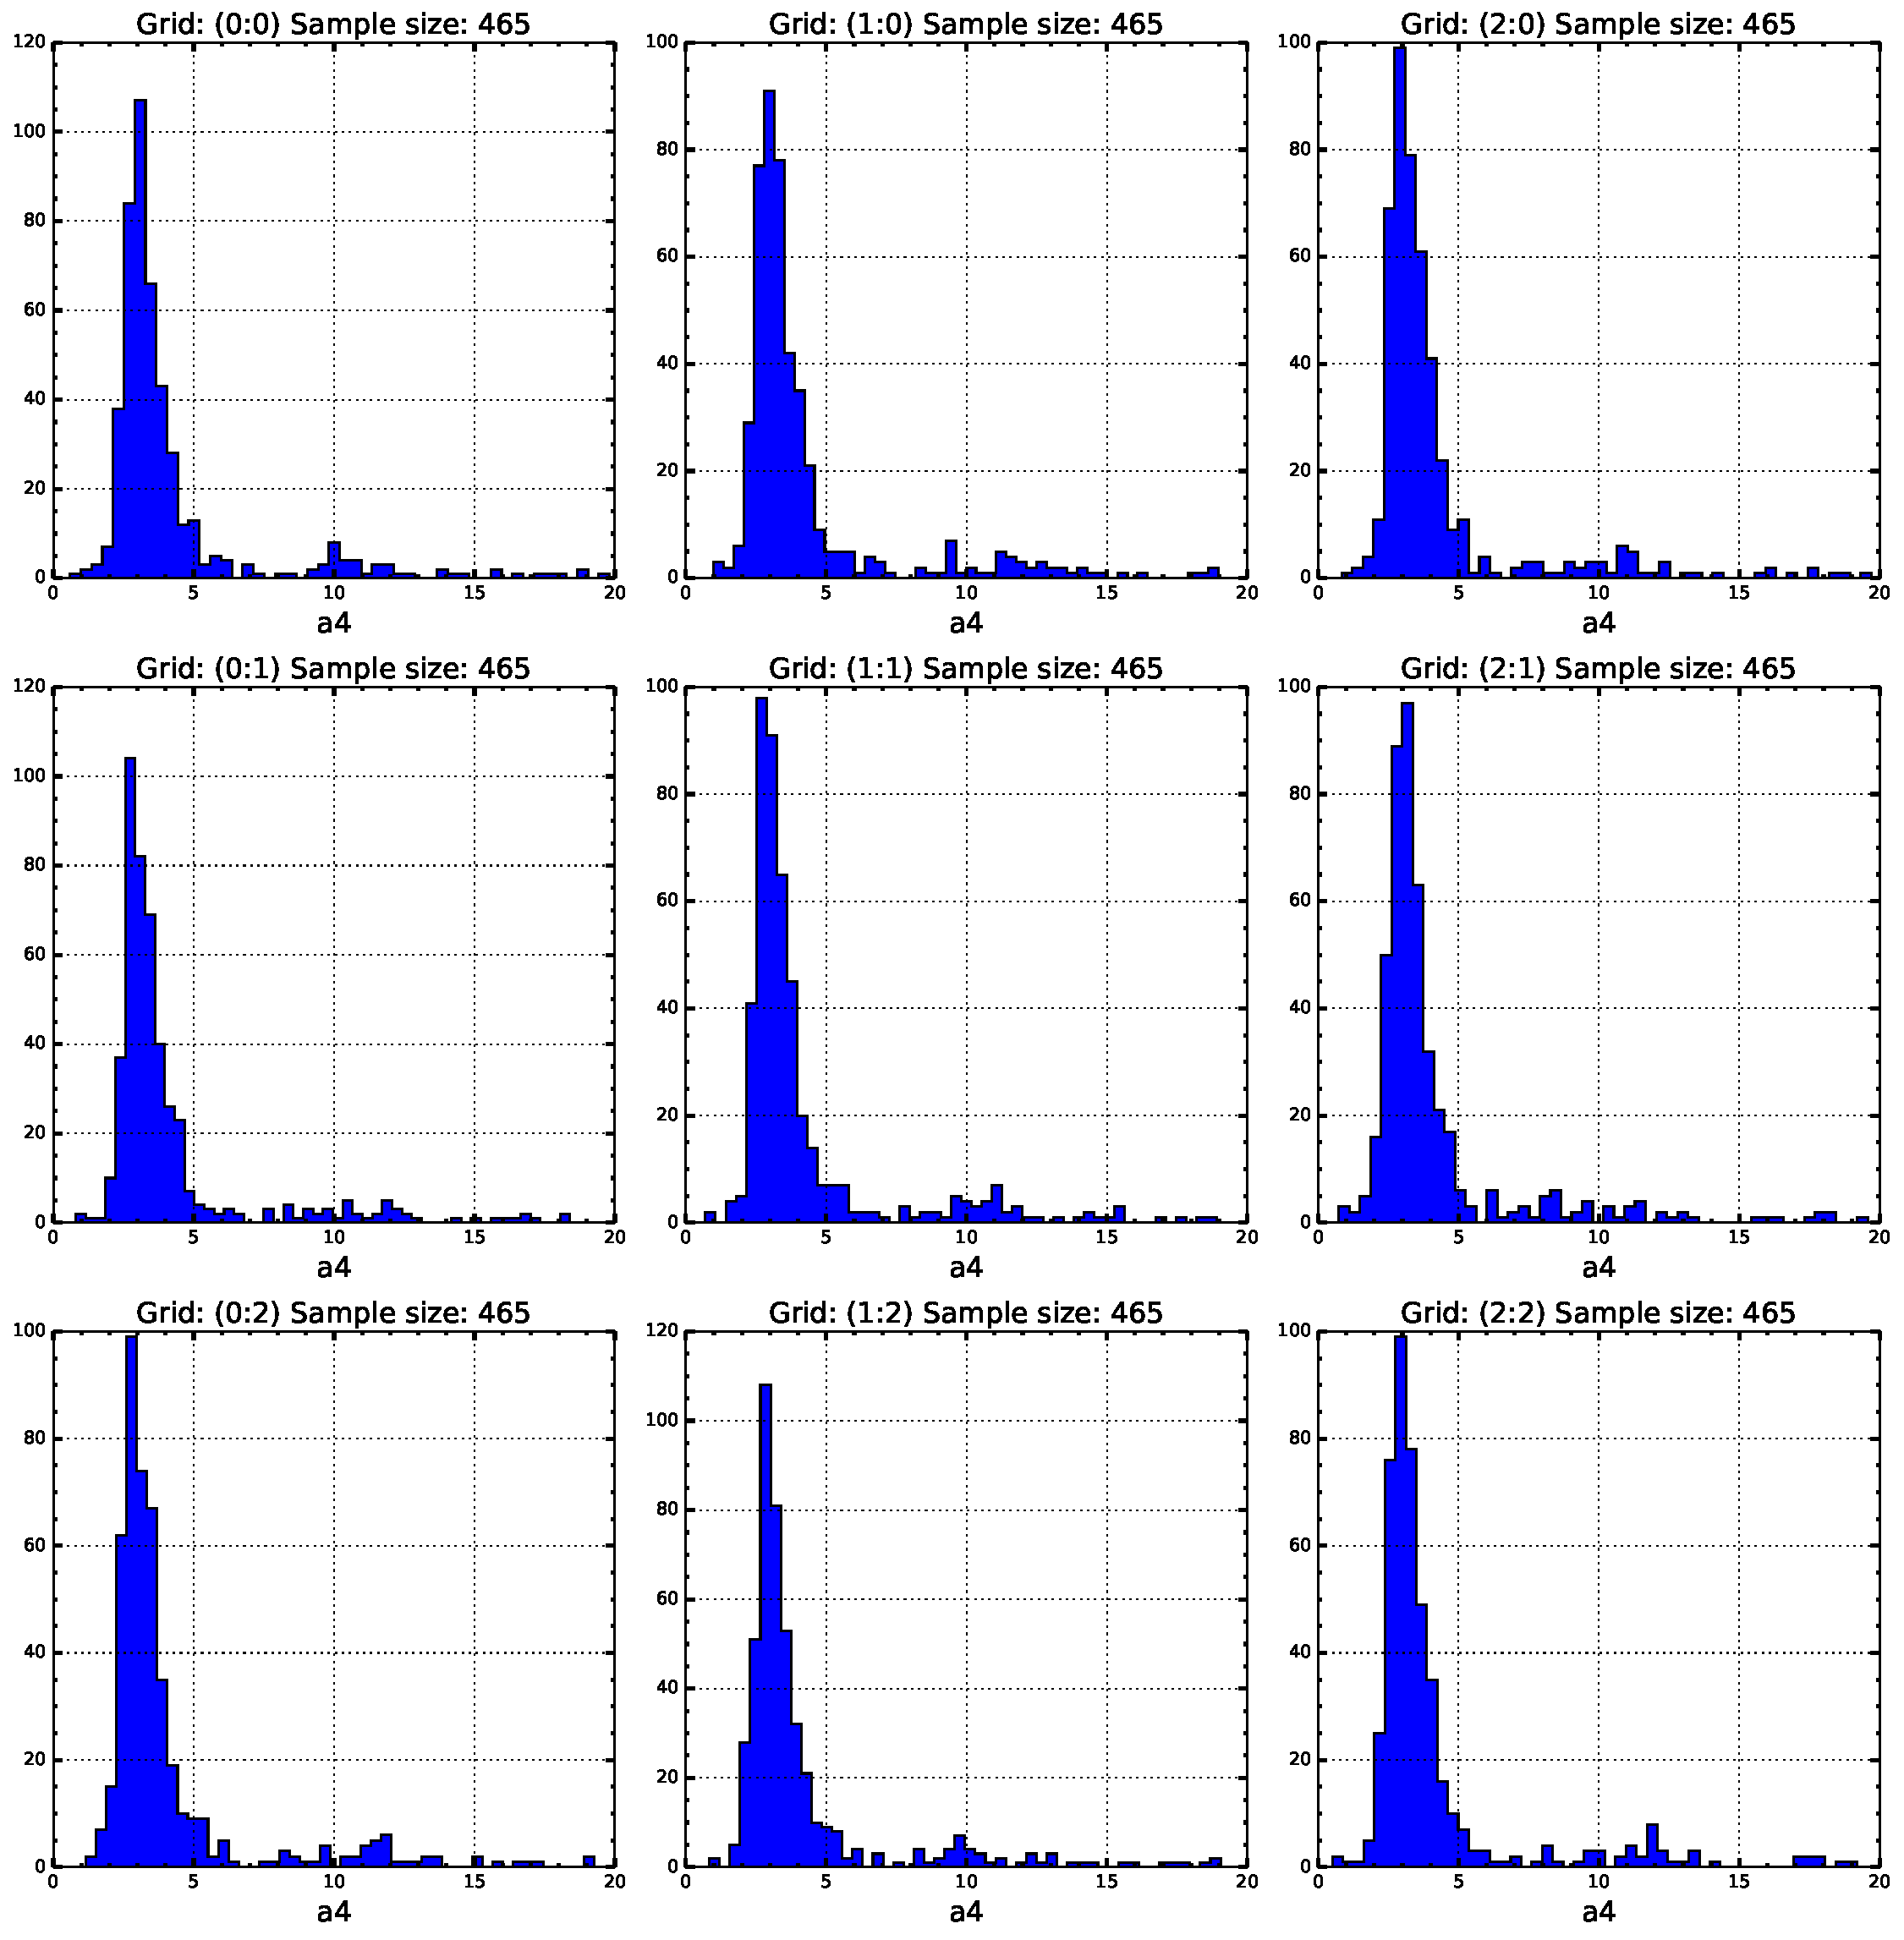
\includegraphics[scale=.42]{psf_dist/a4.pdf}
	\caption[Histogram der Verteilung des PSF-Parameters $A_4$]{Histogram der Verteilung des PSF-Parameters $A_4$}
    \label{psf_dist_a4}
\end{figure}
\begin{figure}[H]
	\centering
	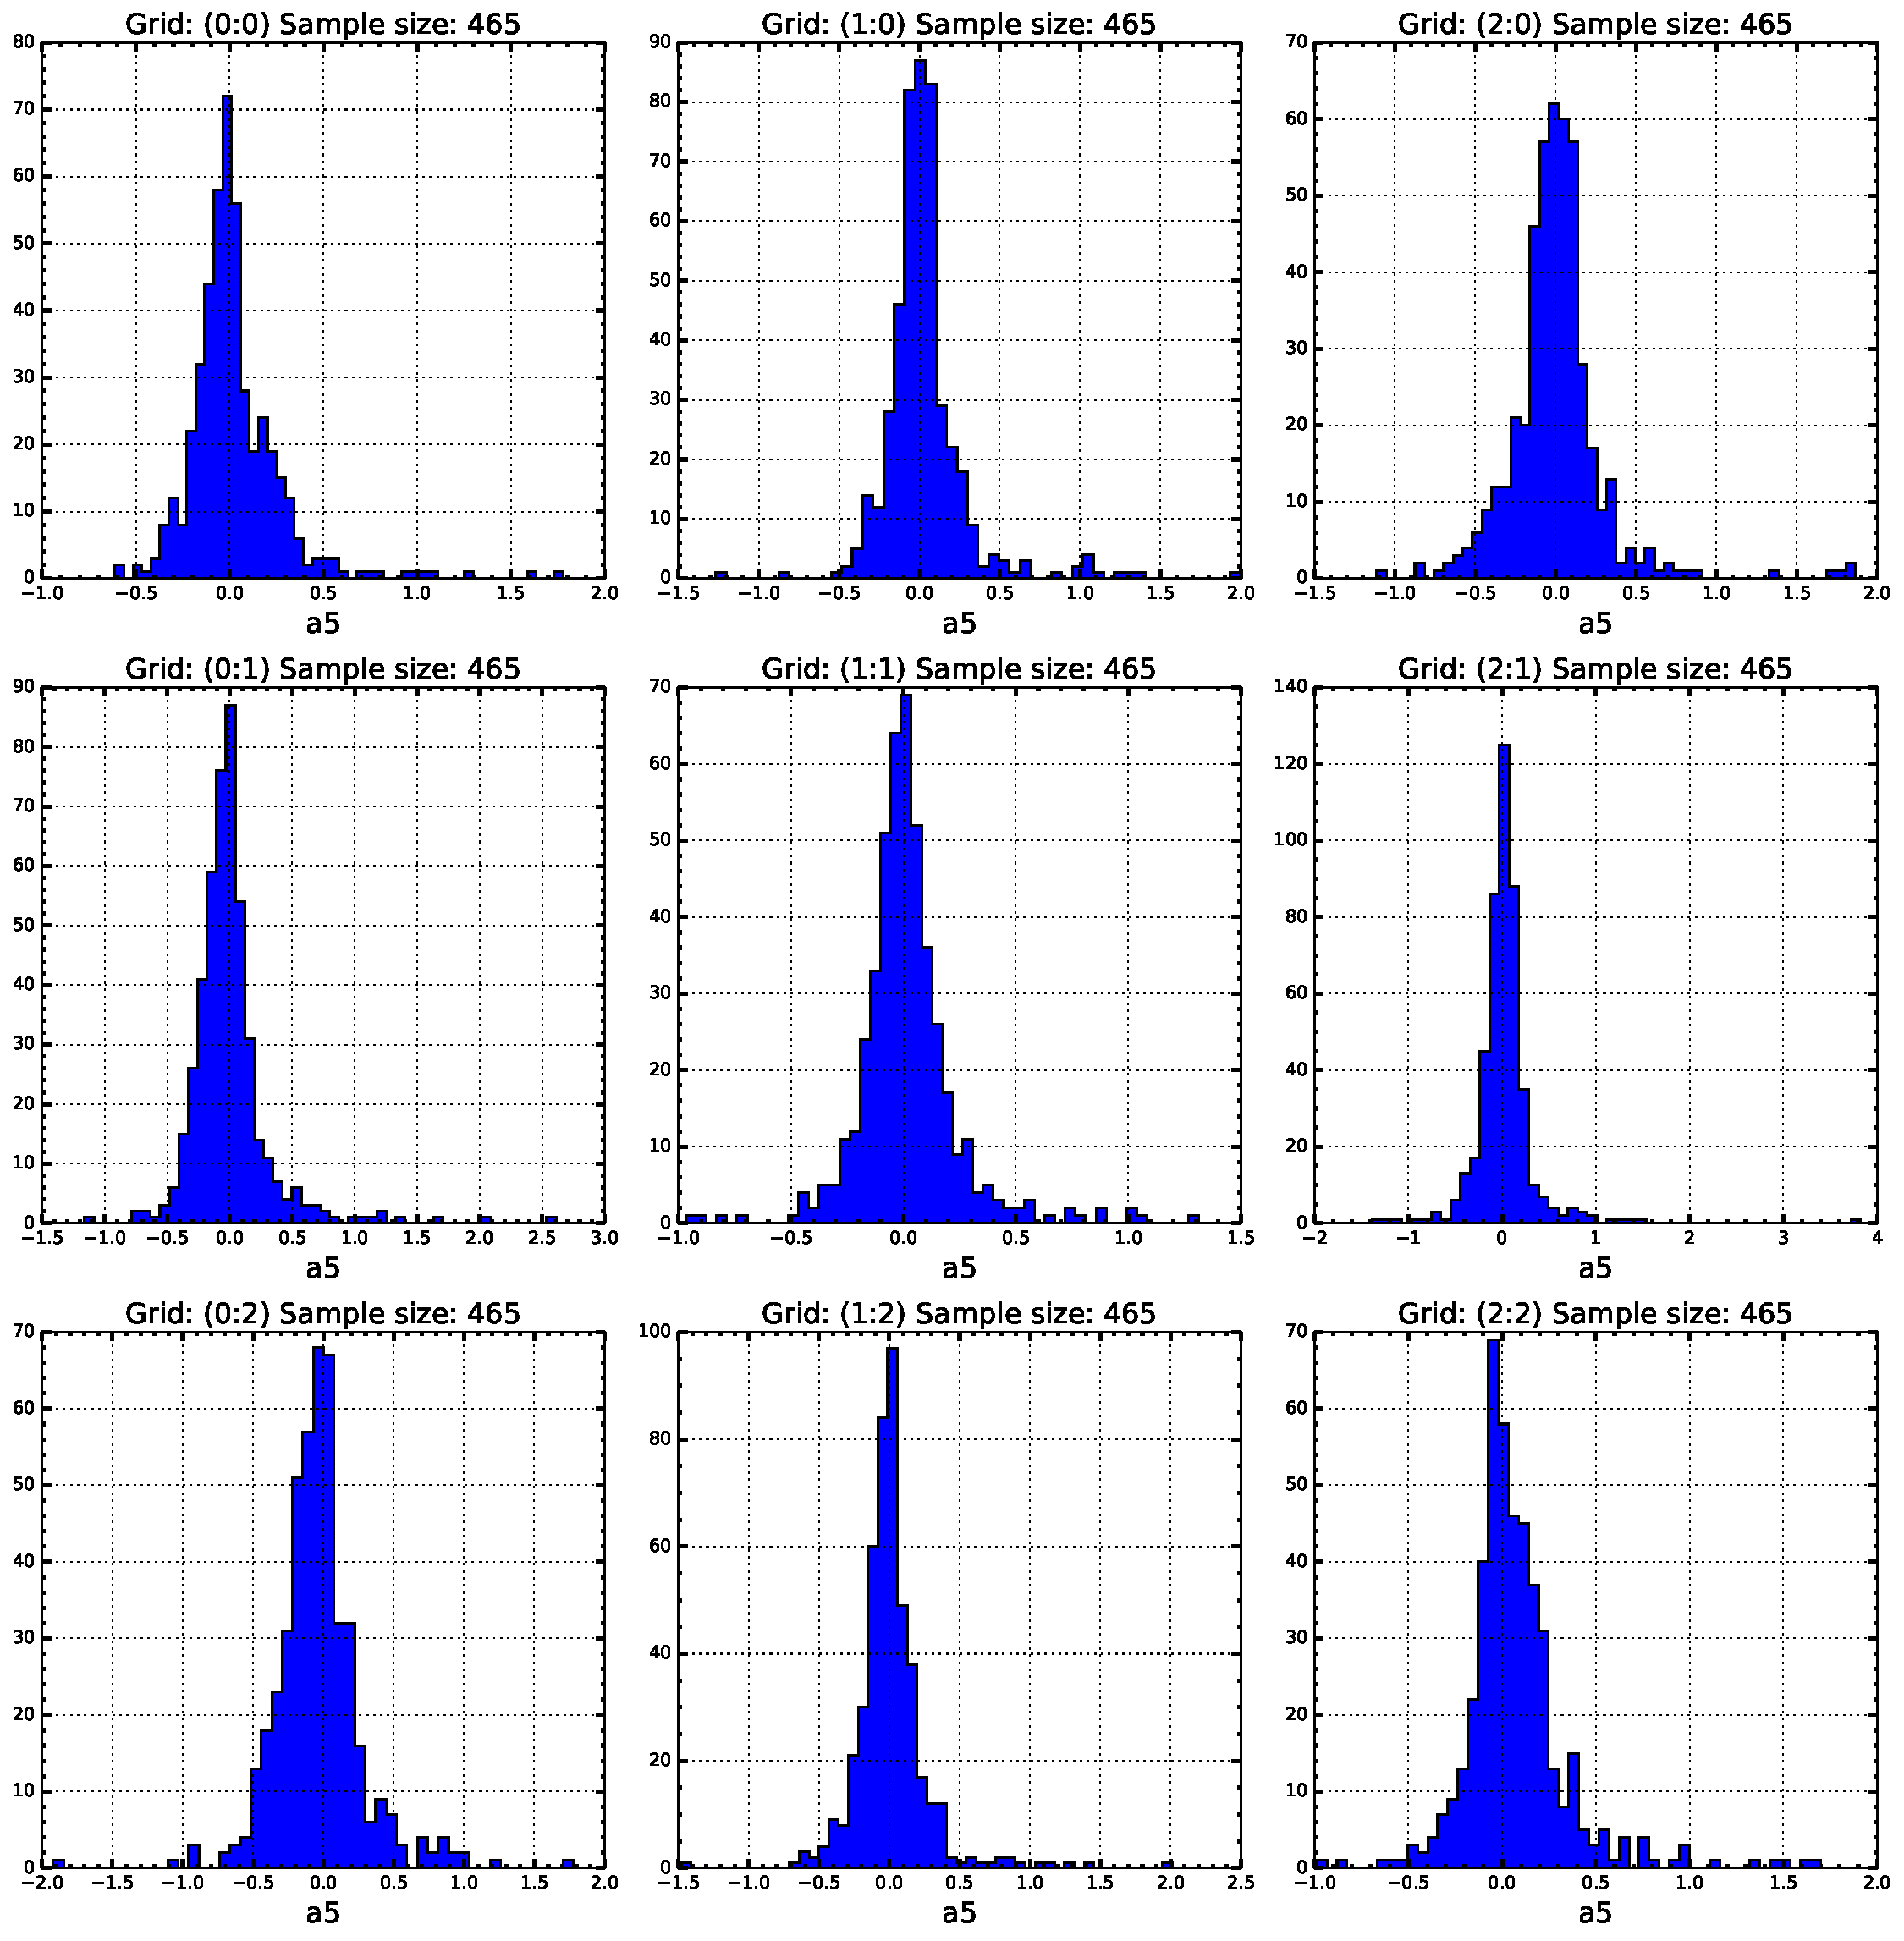
\includegraphics[scale=.42]{psf_dist/a5.pdf}
	\caption[Histogram der Verteilung des PSF-Parameters $A_5$]{Histogram der Verteilung des PSF-Parameters $A_5$}
    \label{psf_dist_a5}
\end{figure}
\begin{figure}[H]
	\centering
	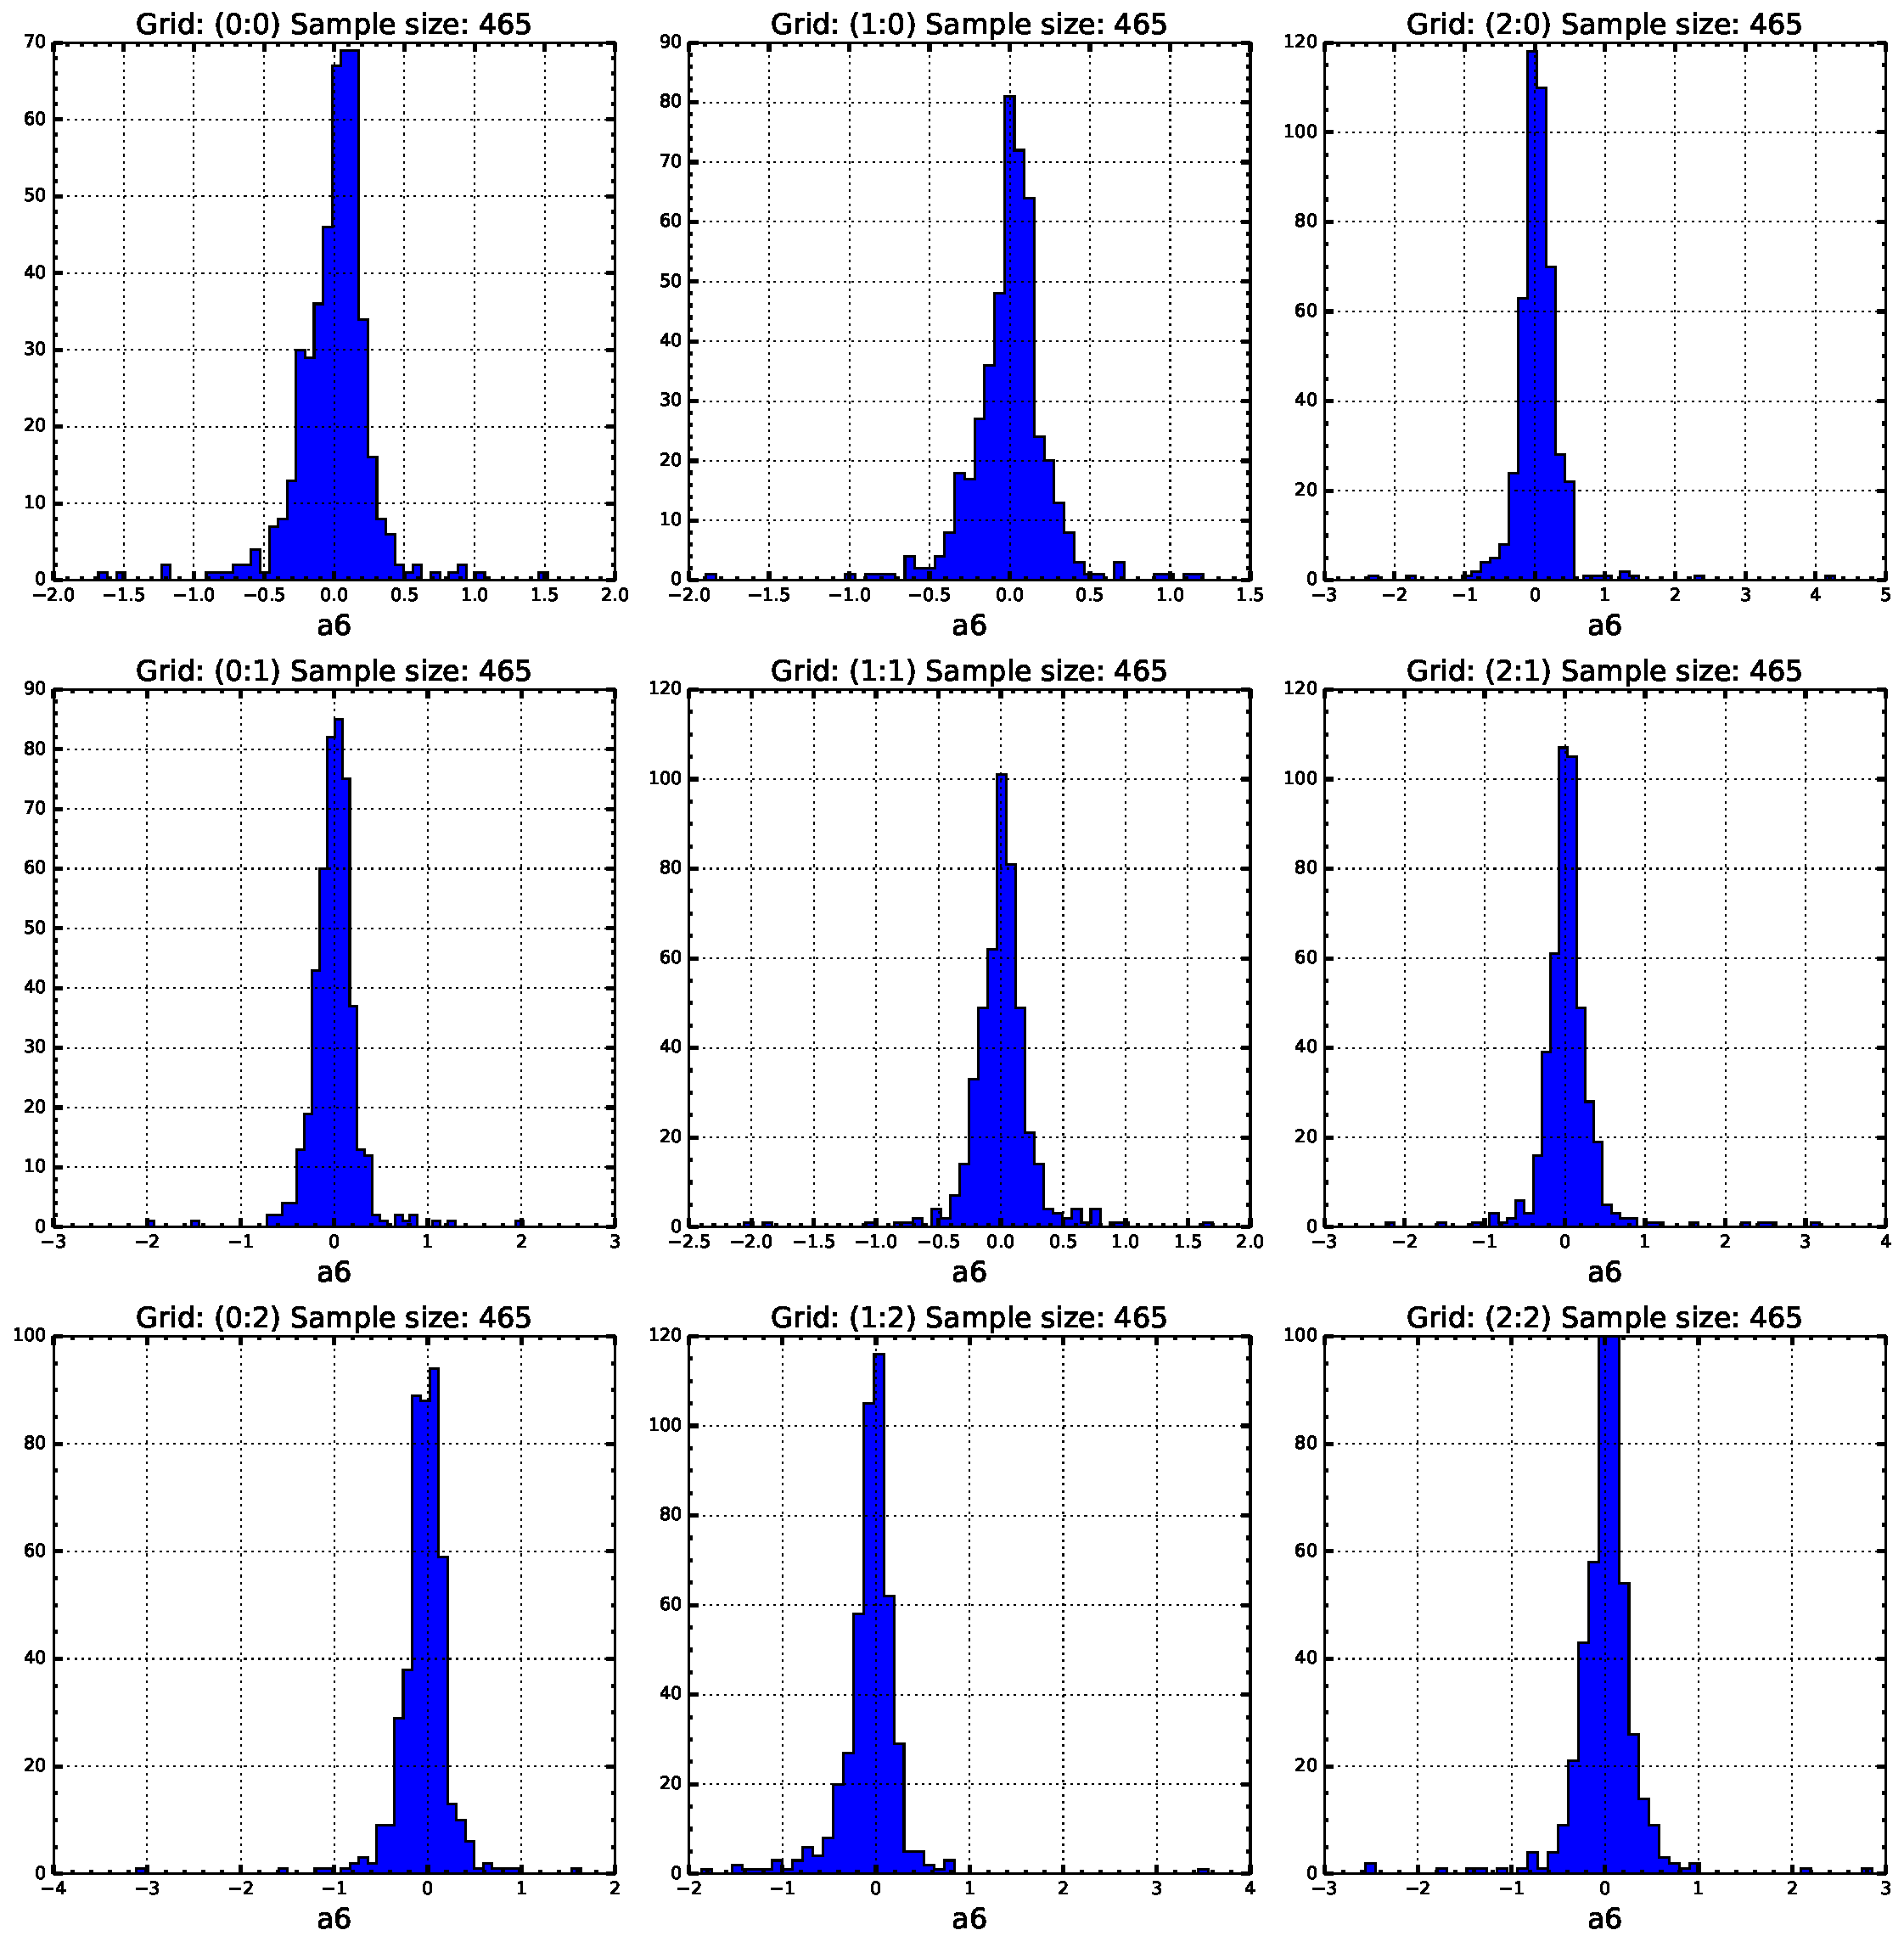
\includegraphics[scale=.42]{psf_dist/a6.pdf}
	\caption[Histogram der Verteilung des PSF-Parameters $A_6$]{Histogram der Verteilung des PSF-Parameters $A_6$}
    \label{psf_dist_a6}
\end{figure}

\section{PSF Temperatur- und Elevationsabhängigkeiten}
\begin{figure}[H]
	\centering
	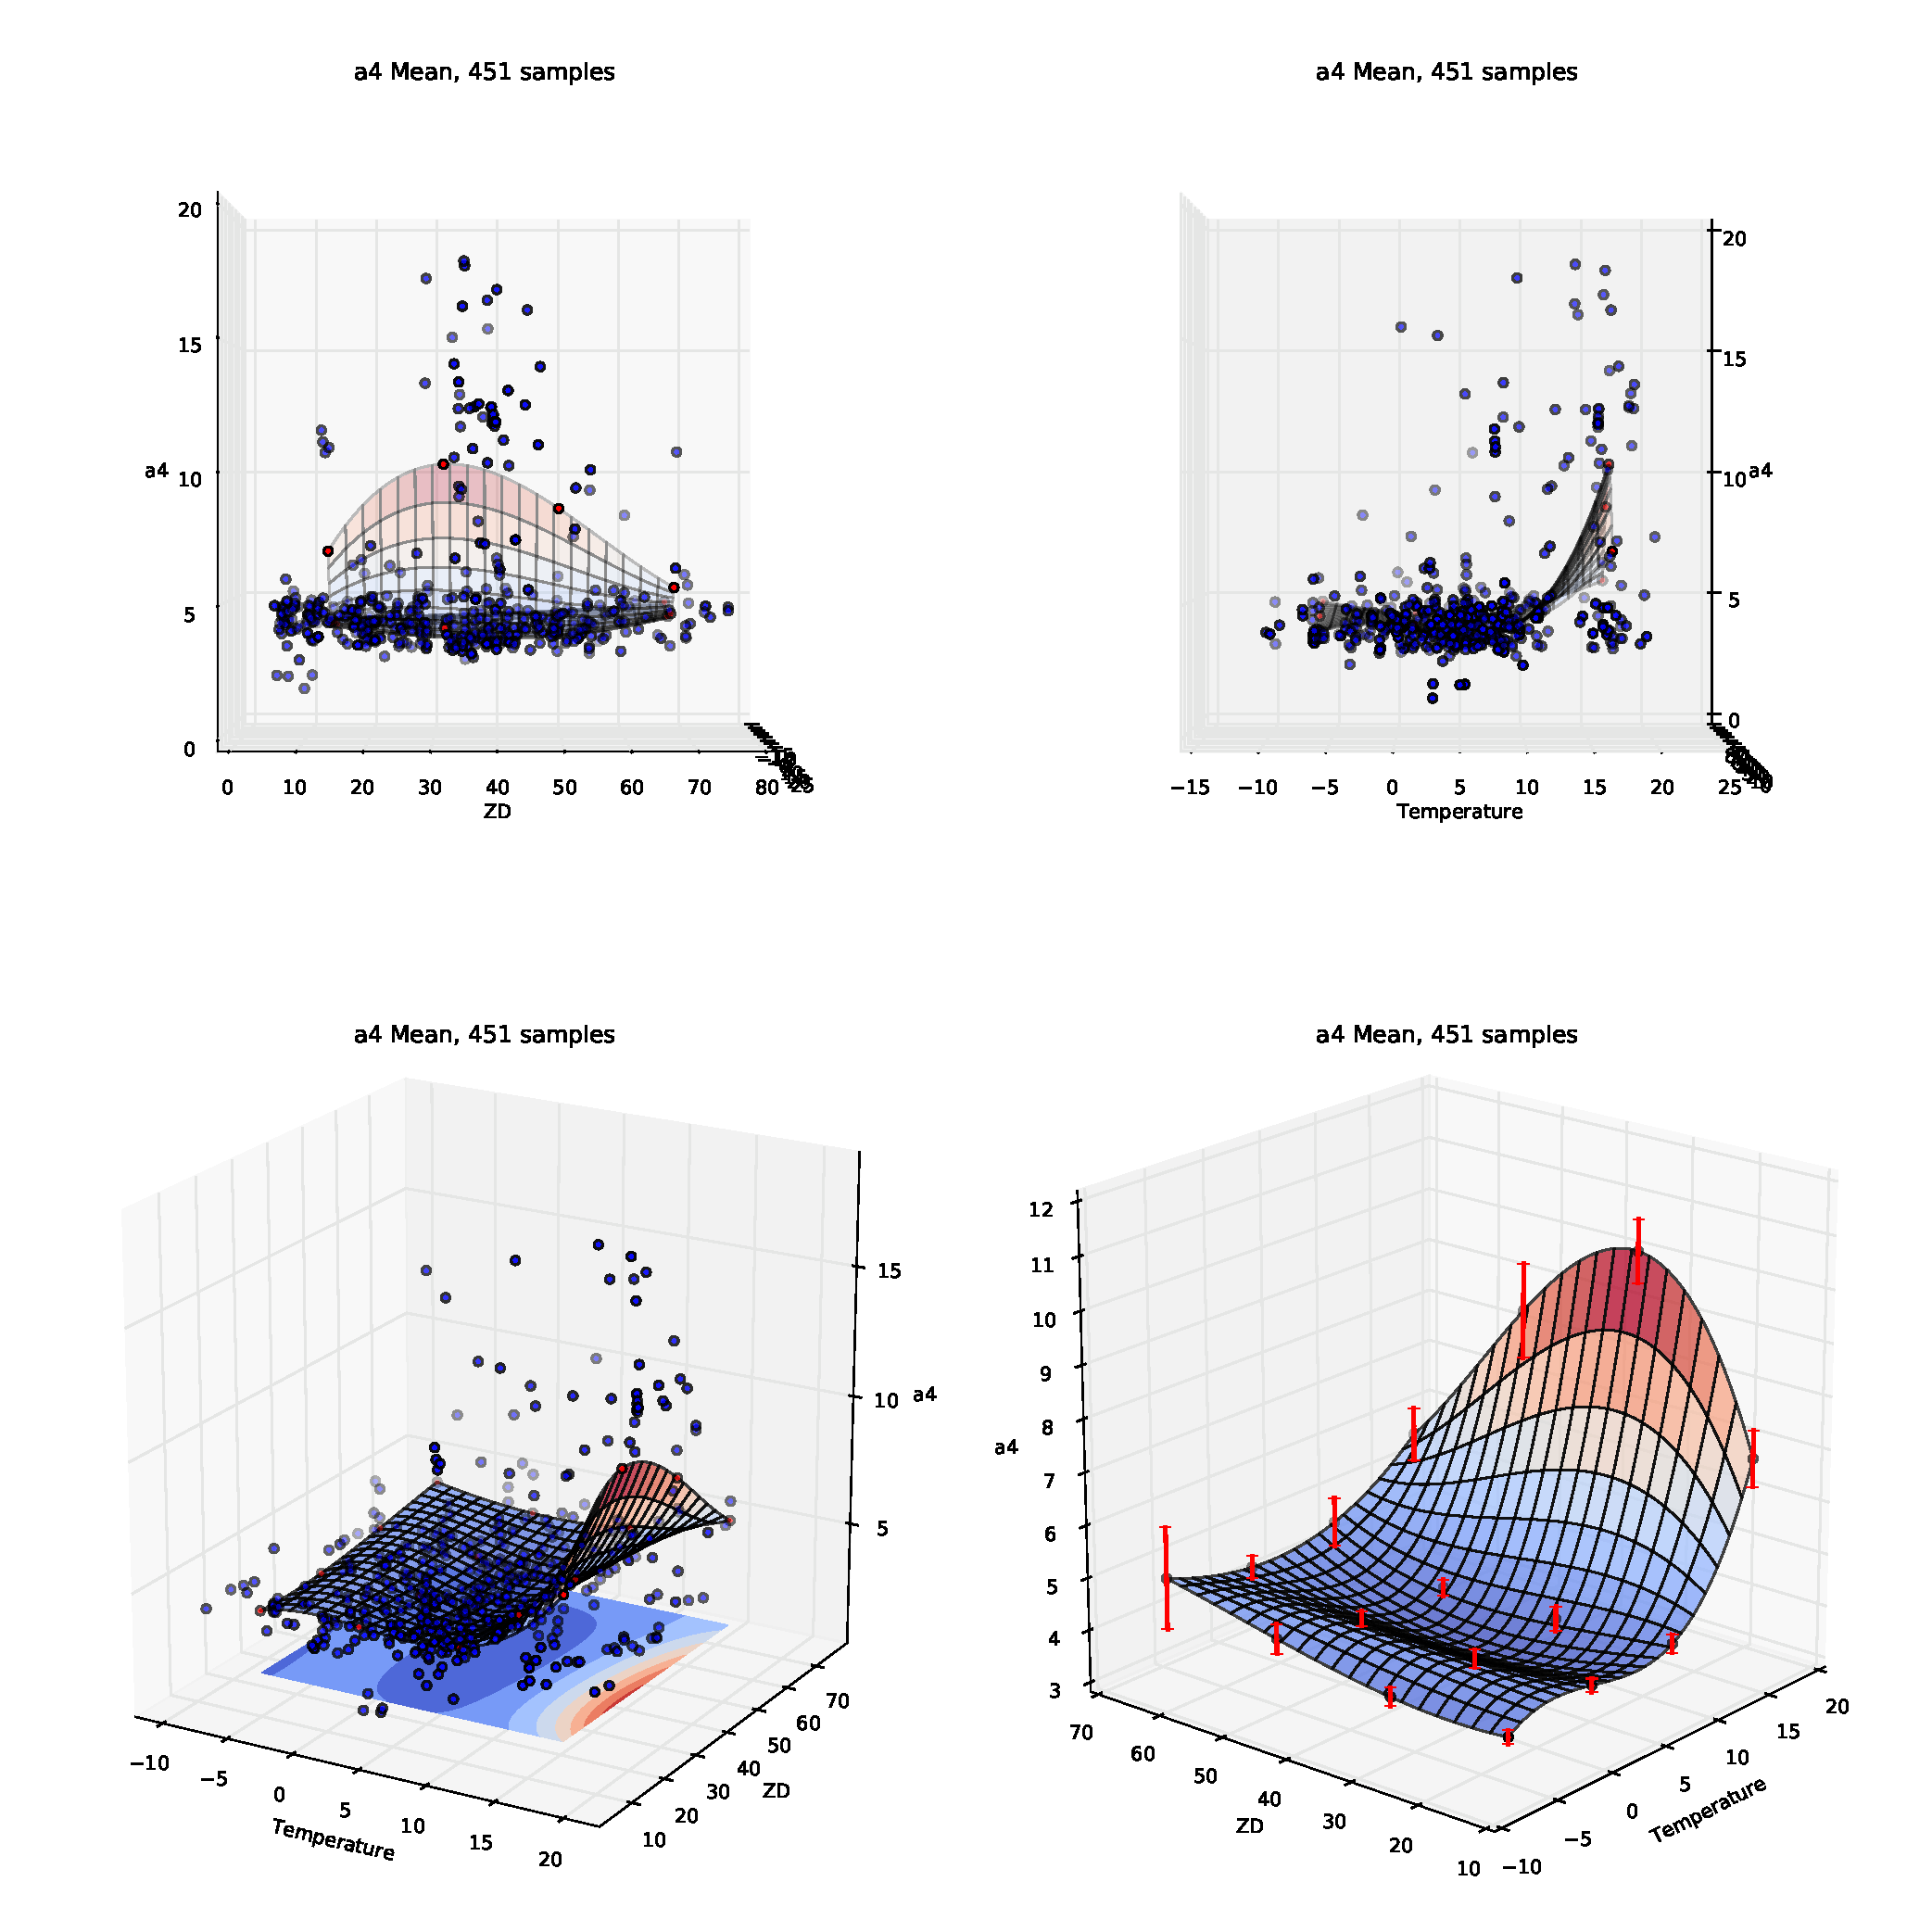
\includegraphics[scale=.48]{psf_surf/a4_mean.pdf}
	\caption[Mean Streu- und Flächenplot des PSF-Parameters $A_4$]{Mean Streu- und Flächenplot des PSF-Parameters $A_4$}
    \label{psf_surf_a4_mean}
\end{figure}
\begin{figure}[H]
	\centering
	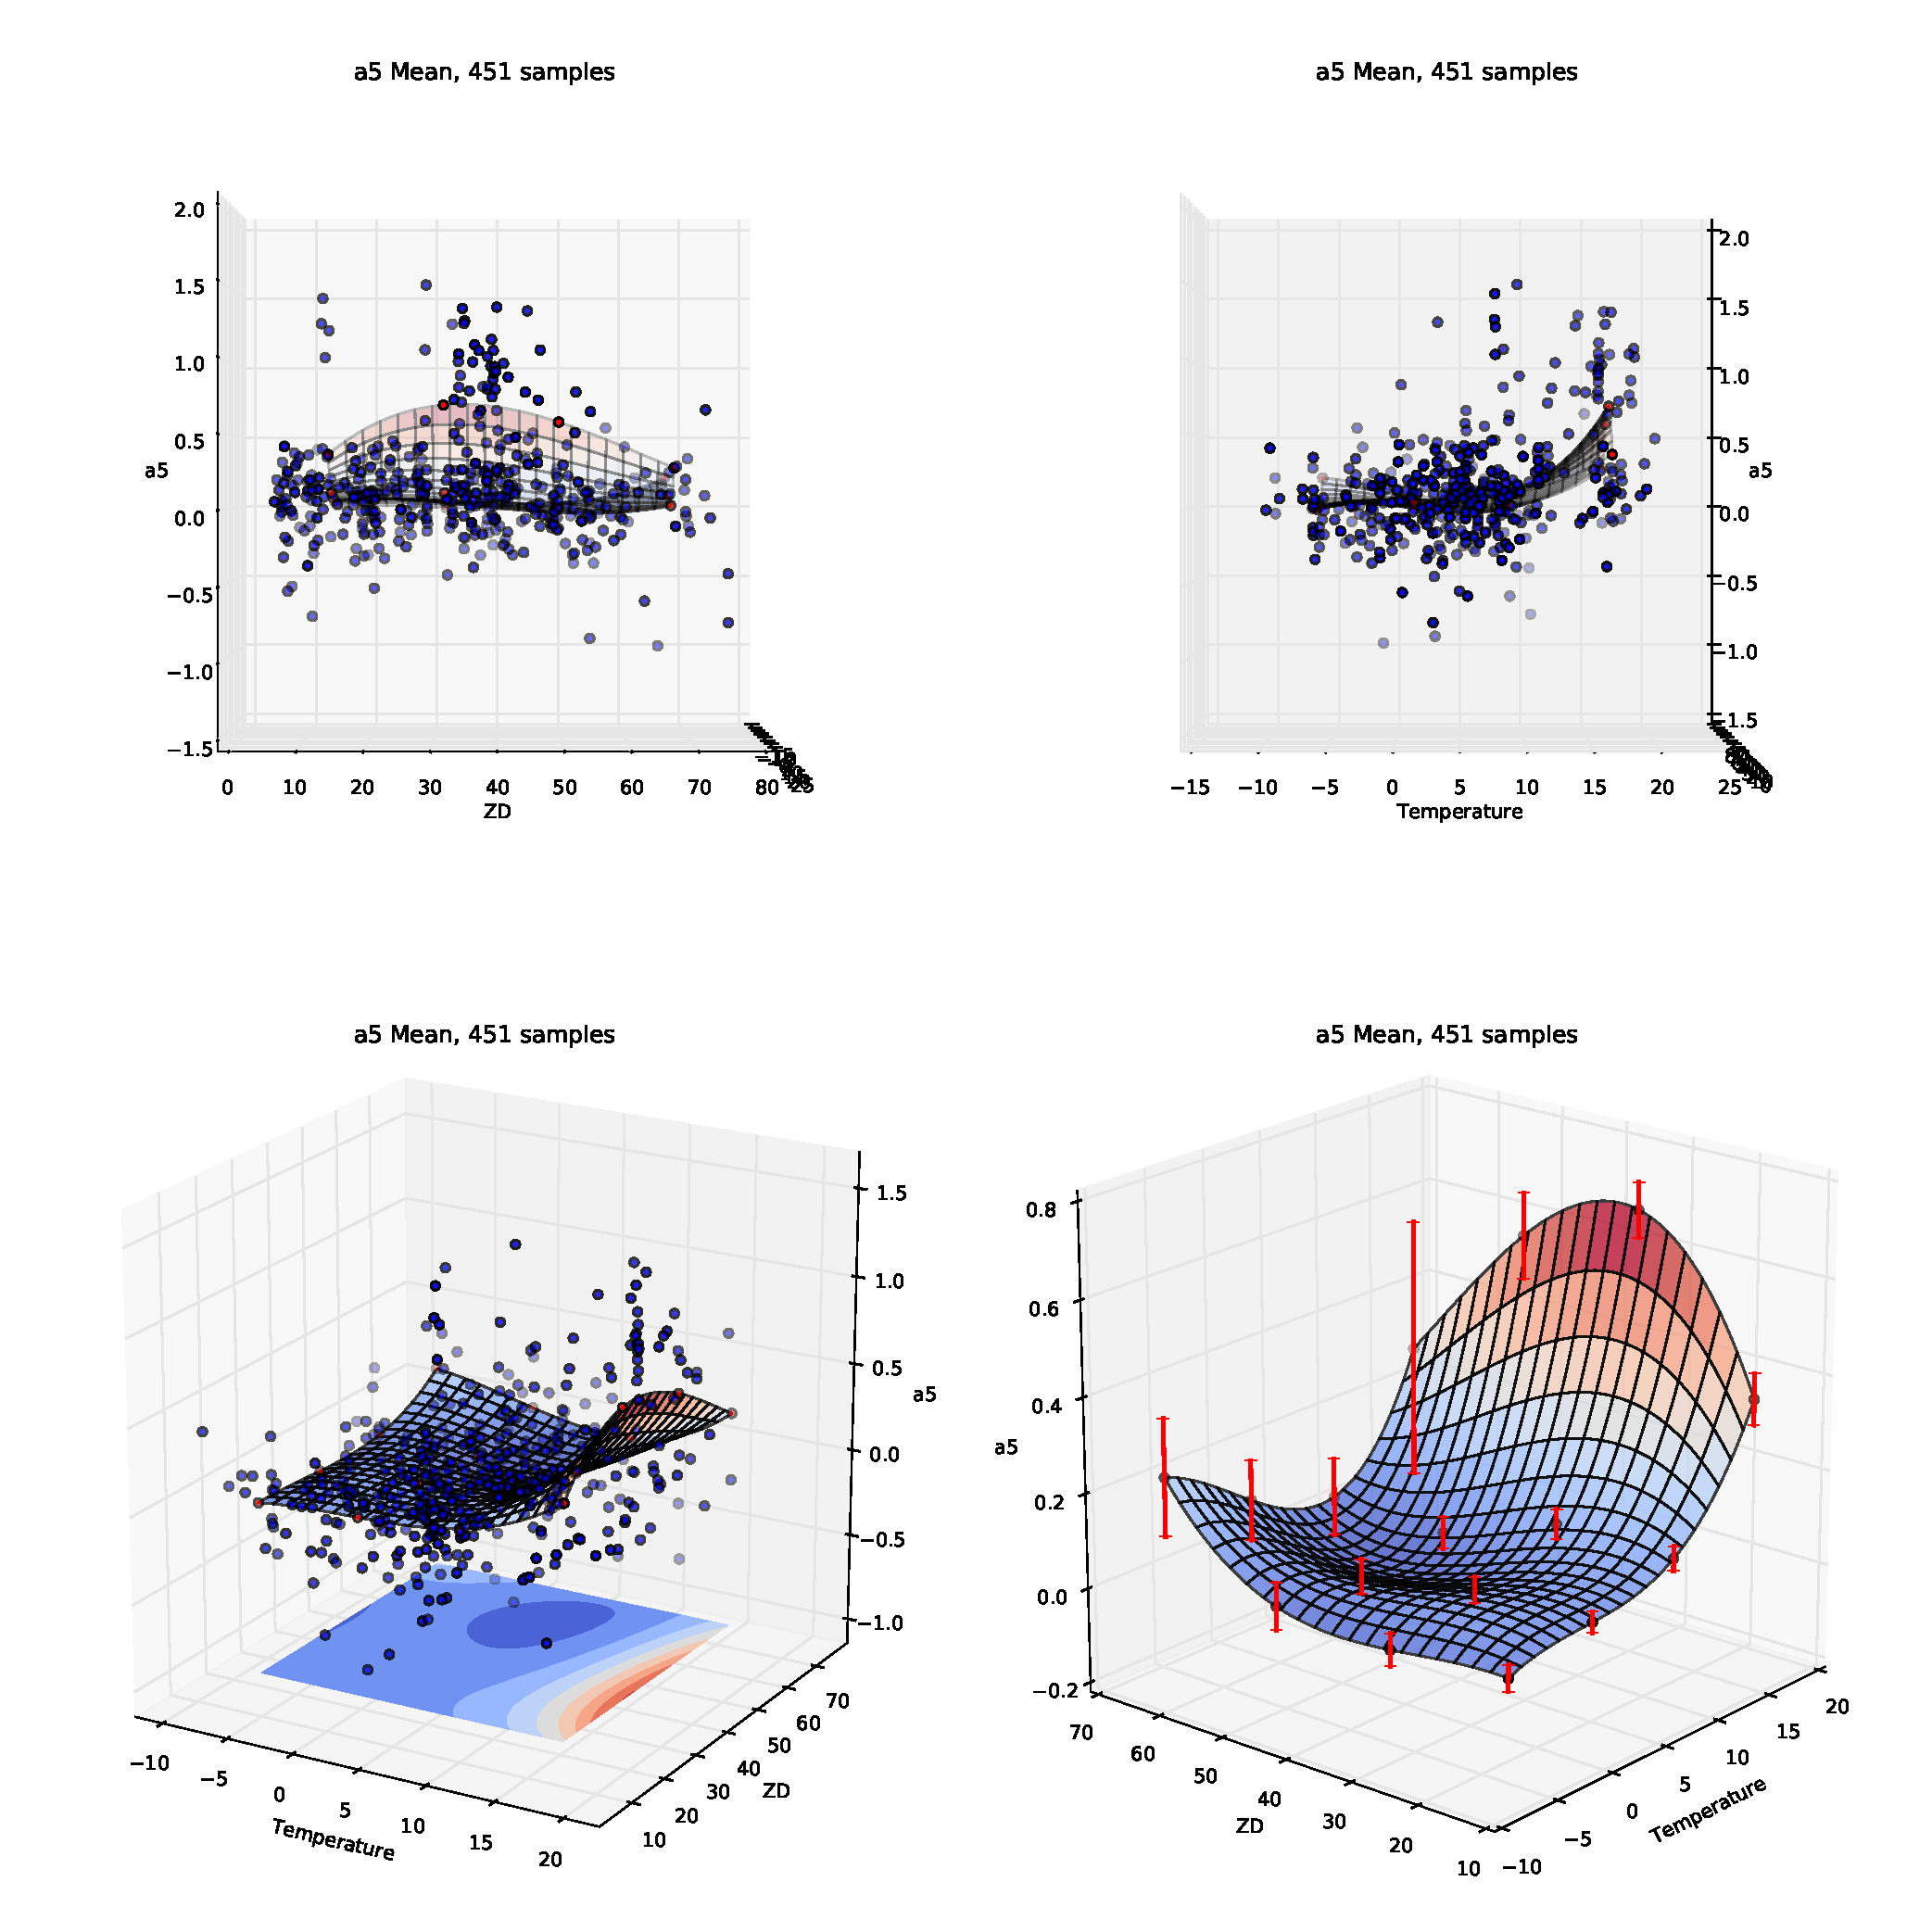
\includegraphics[scale=.48]{psf_surf/a5_mean.pdf}
	\caption[Mean Streu- und Flächenplot des PSF-Parameters $A_5$]{Mean Streu- und Flächenplot des PSF-Parameters $A_5$}
    \label{psf_surf_a5_mean}
\end{figure}
\begin{figure}[H]
	\centering
	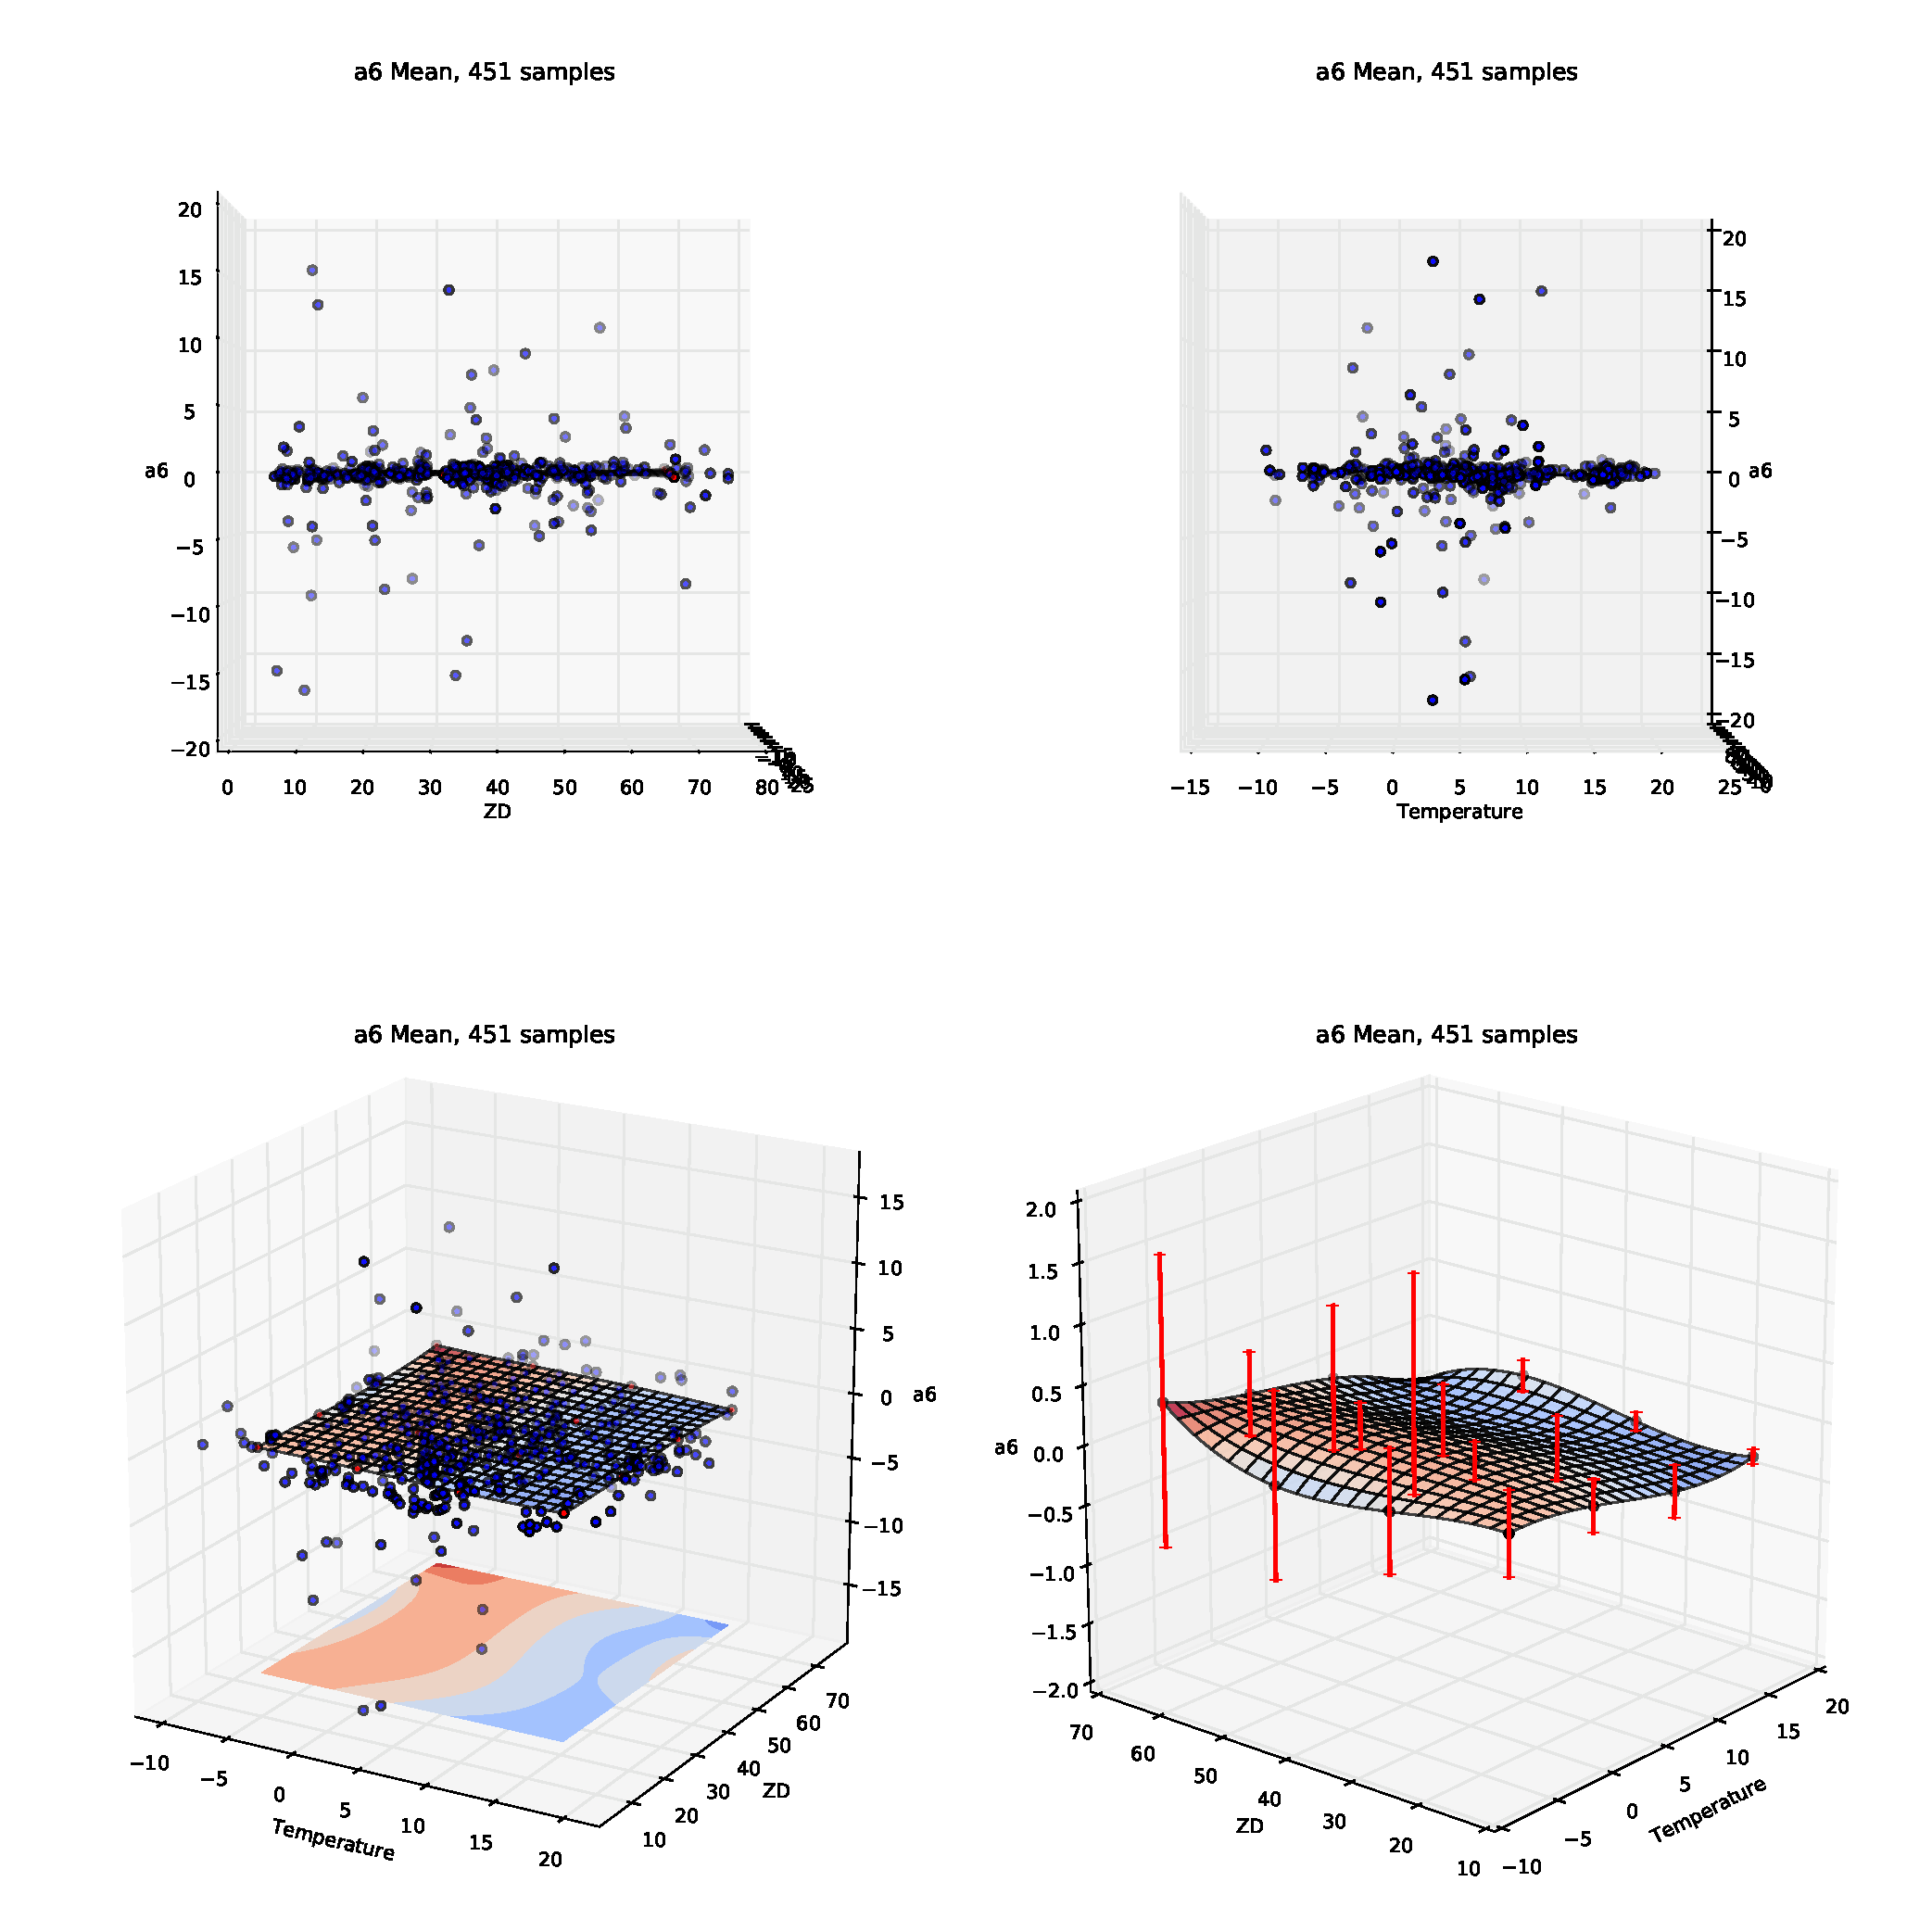
\includegraphics[scale=.48]{psf_surf/a6_mean.pdf}
	\caption[Mean Streu- und Flächenplot des PSF-Parameters $A_6$]{Mean Streu- und Flächenplot des PSF-Parameters $A_6$}
    \label{psf_surf_a6_mean}
\end{figure}

\begin{figure}[H]
	\centering
	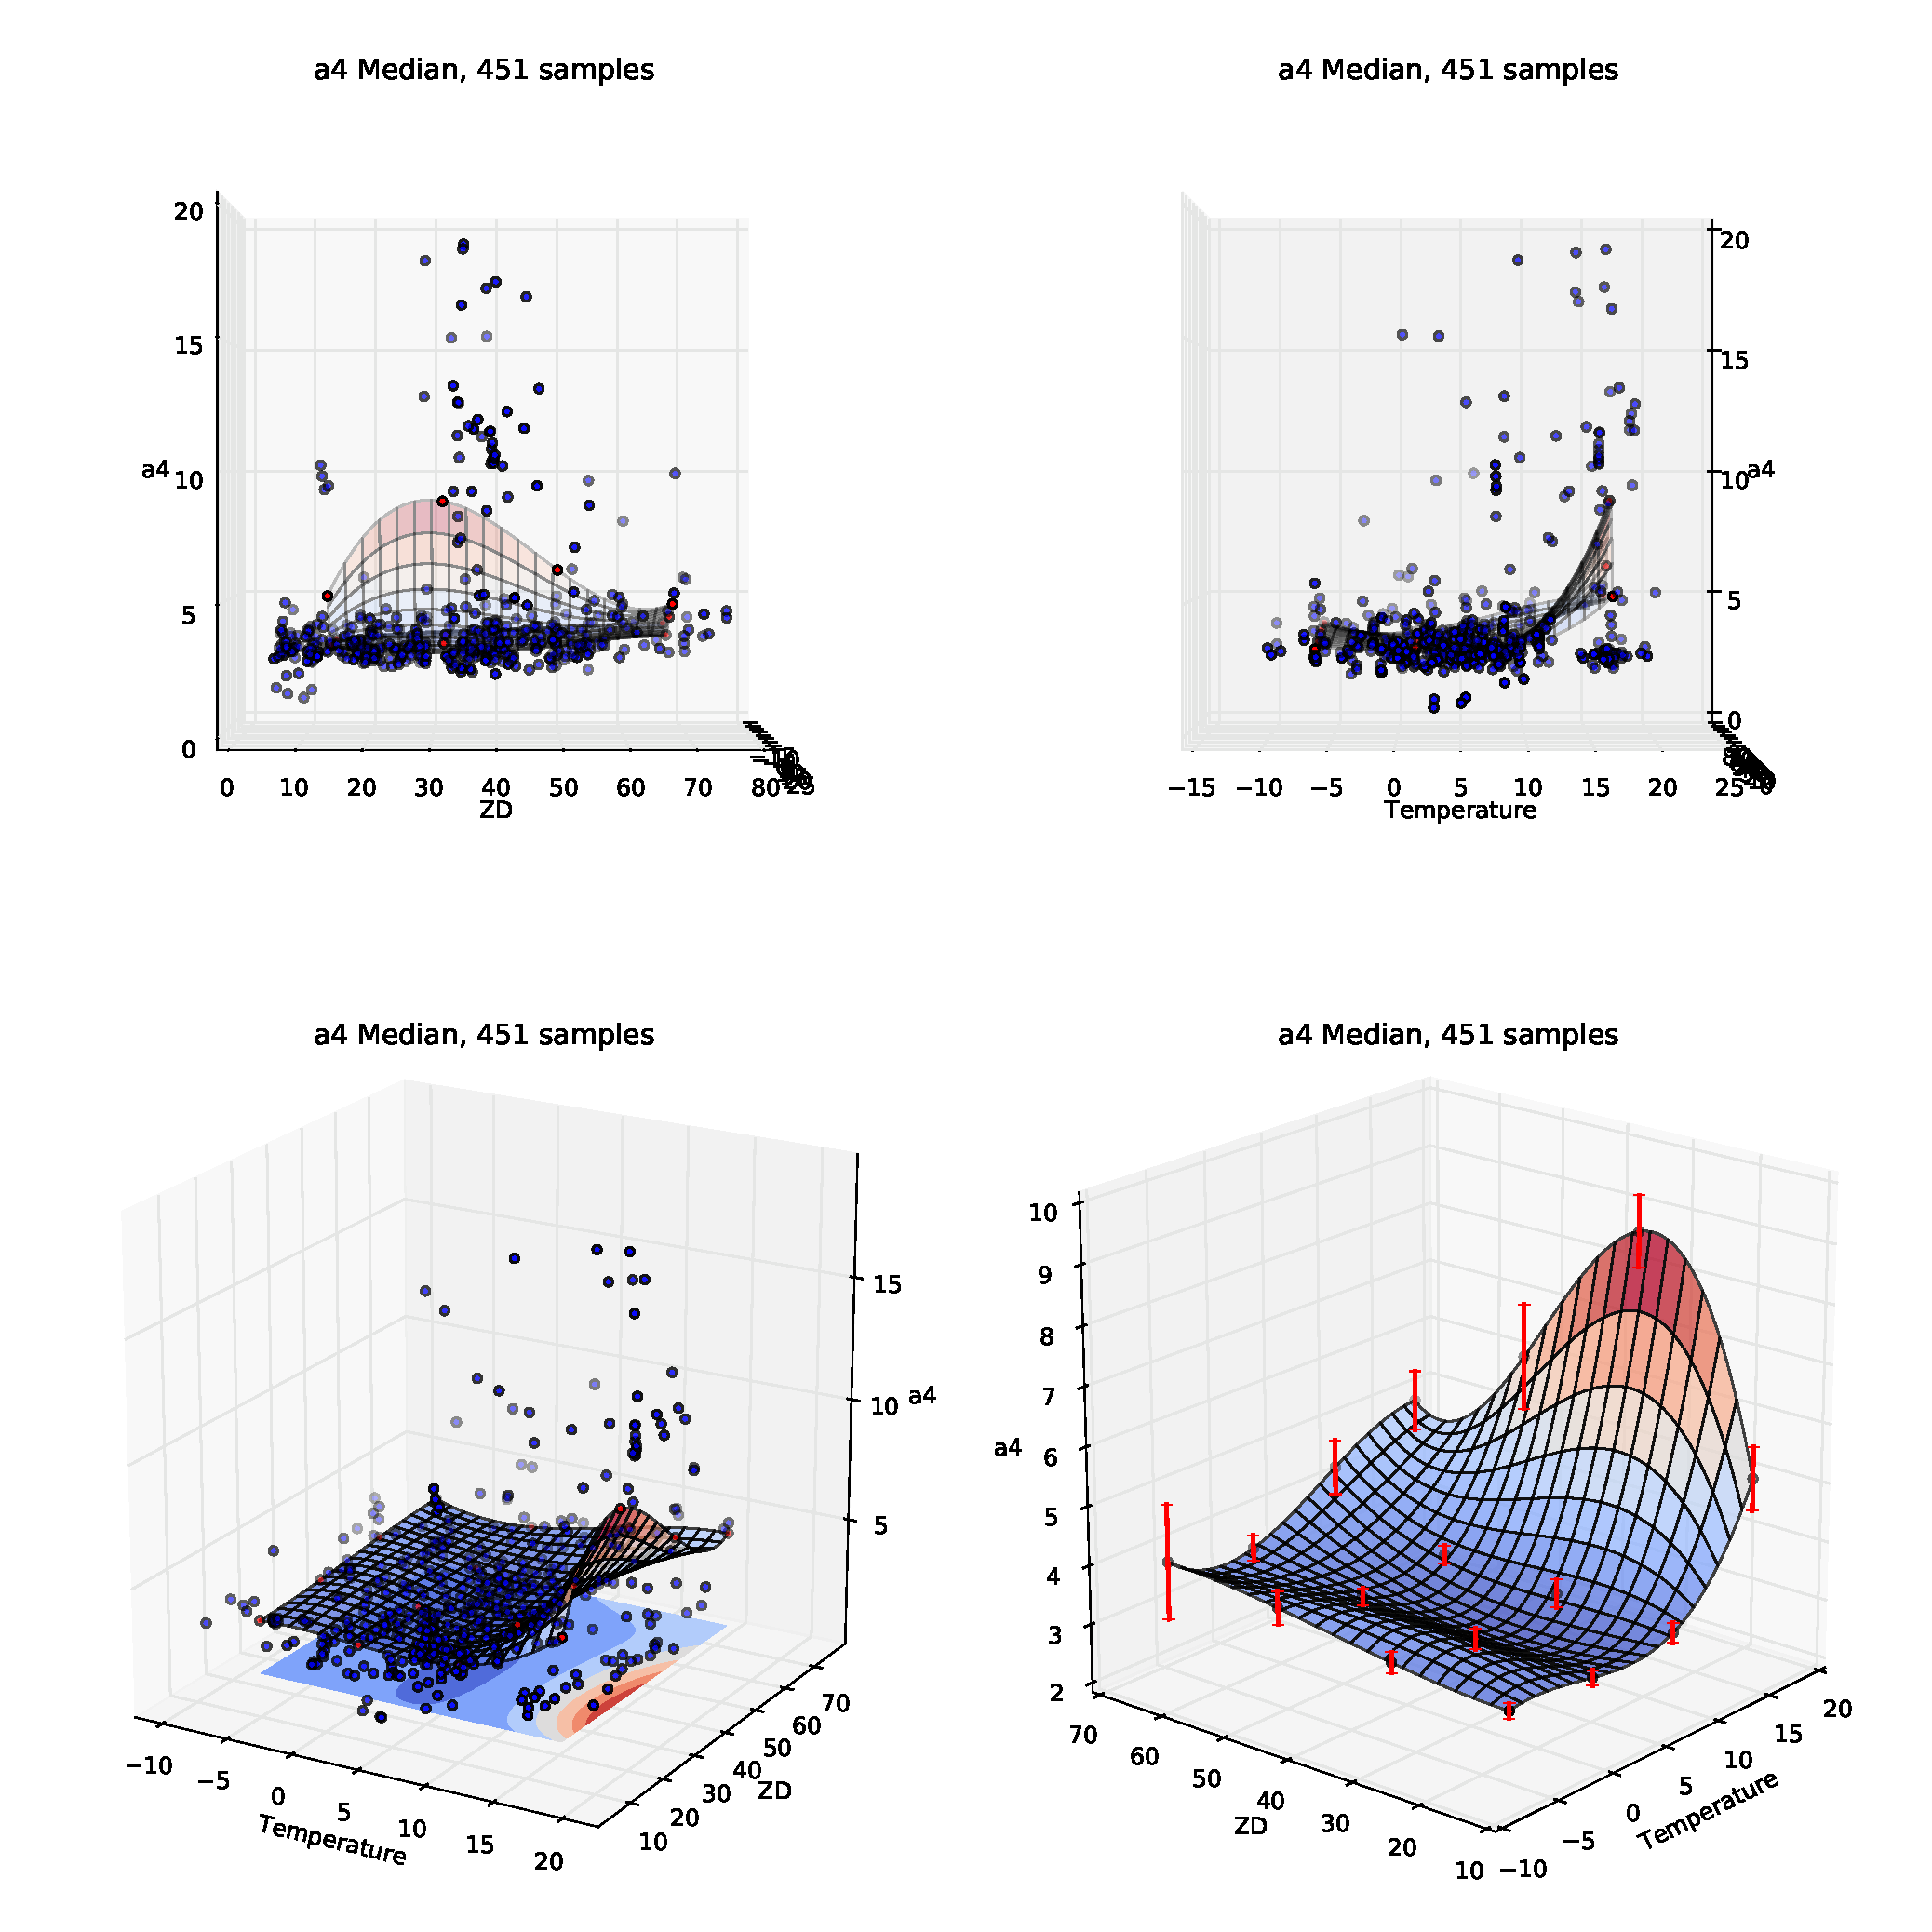
\includegraphics[scale=.48]{psf_surf/a4_med.pdf}
	\caption[Median Streu- und Flächenplot des PSF-Parameters $A_4$]{Median Streu- und Flächenplot des PSF-Parameters $A_4$}
    \label{psf_surf_a4_med}
\end{figure}
\begin{figure}[H]
	\centering
	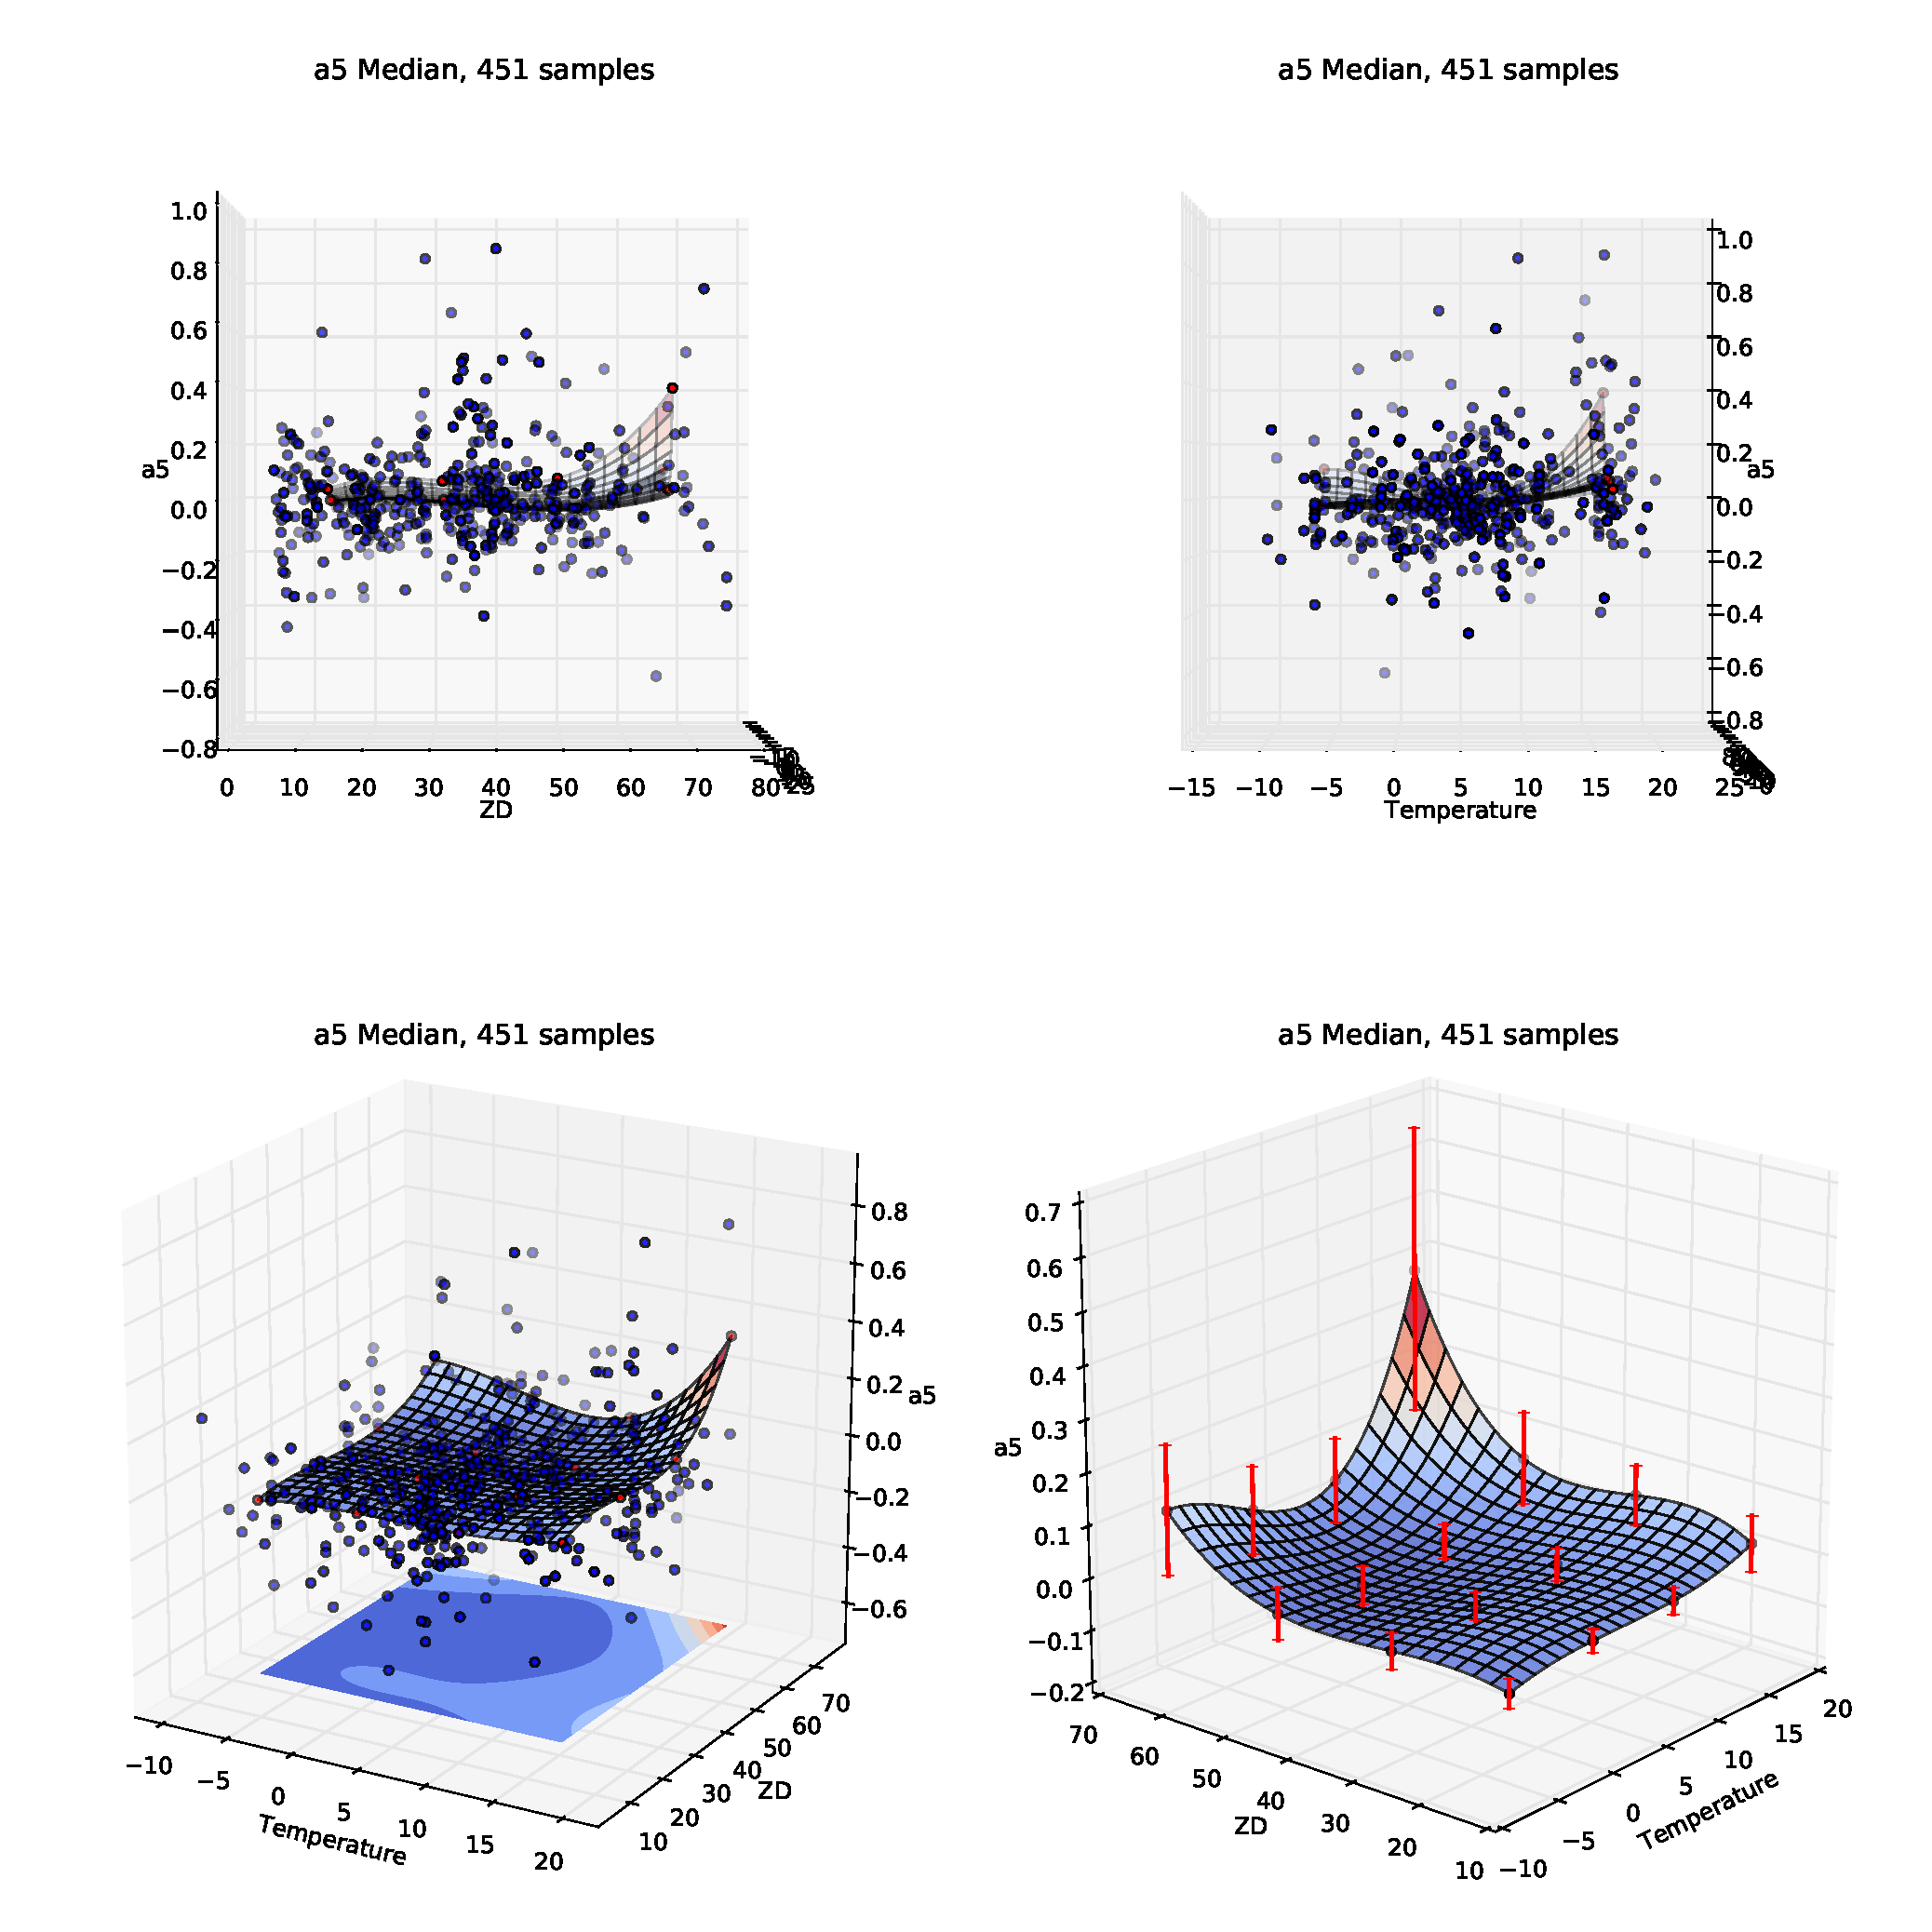
\includegraphics[scale=.48]{psf_surf/a5_med.pdf}
	\caption[Median Streu- und Flächenplot des PSF-Parameters $A_5$]{Median Streu- und Flächenplot des PSF-Parameters $A_5$}
    \label{psf_surf_a5_med}
\end{figure}
\begin{figure}[H]
	\centering
	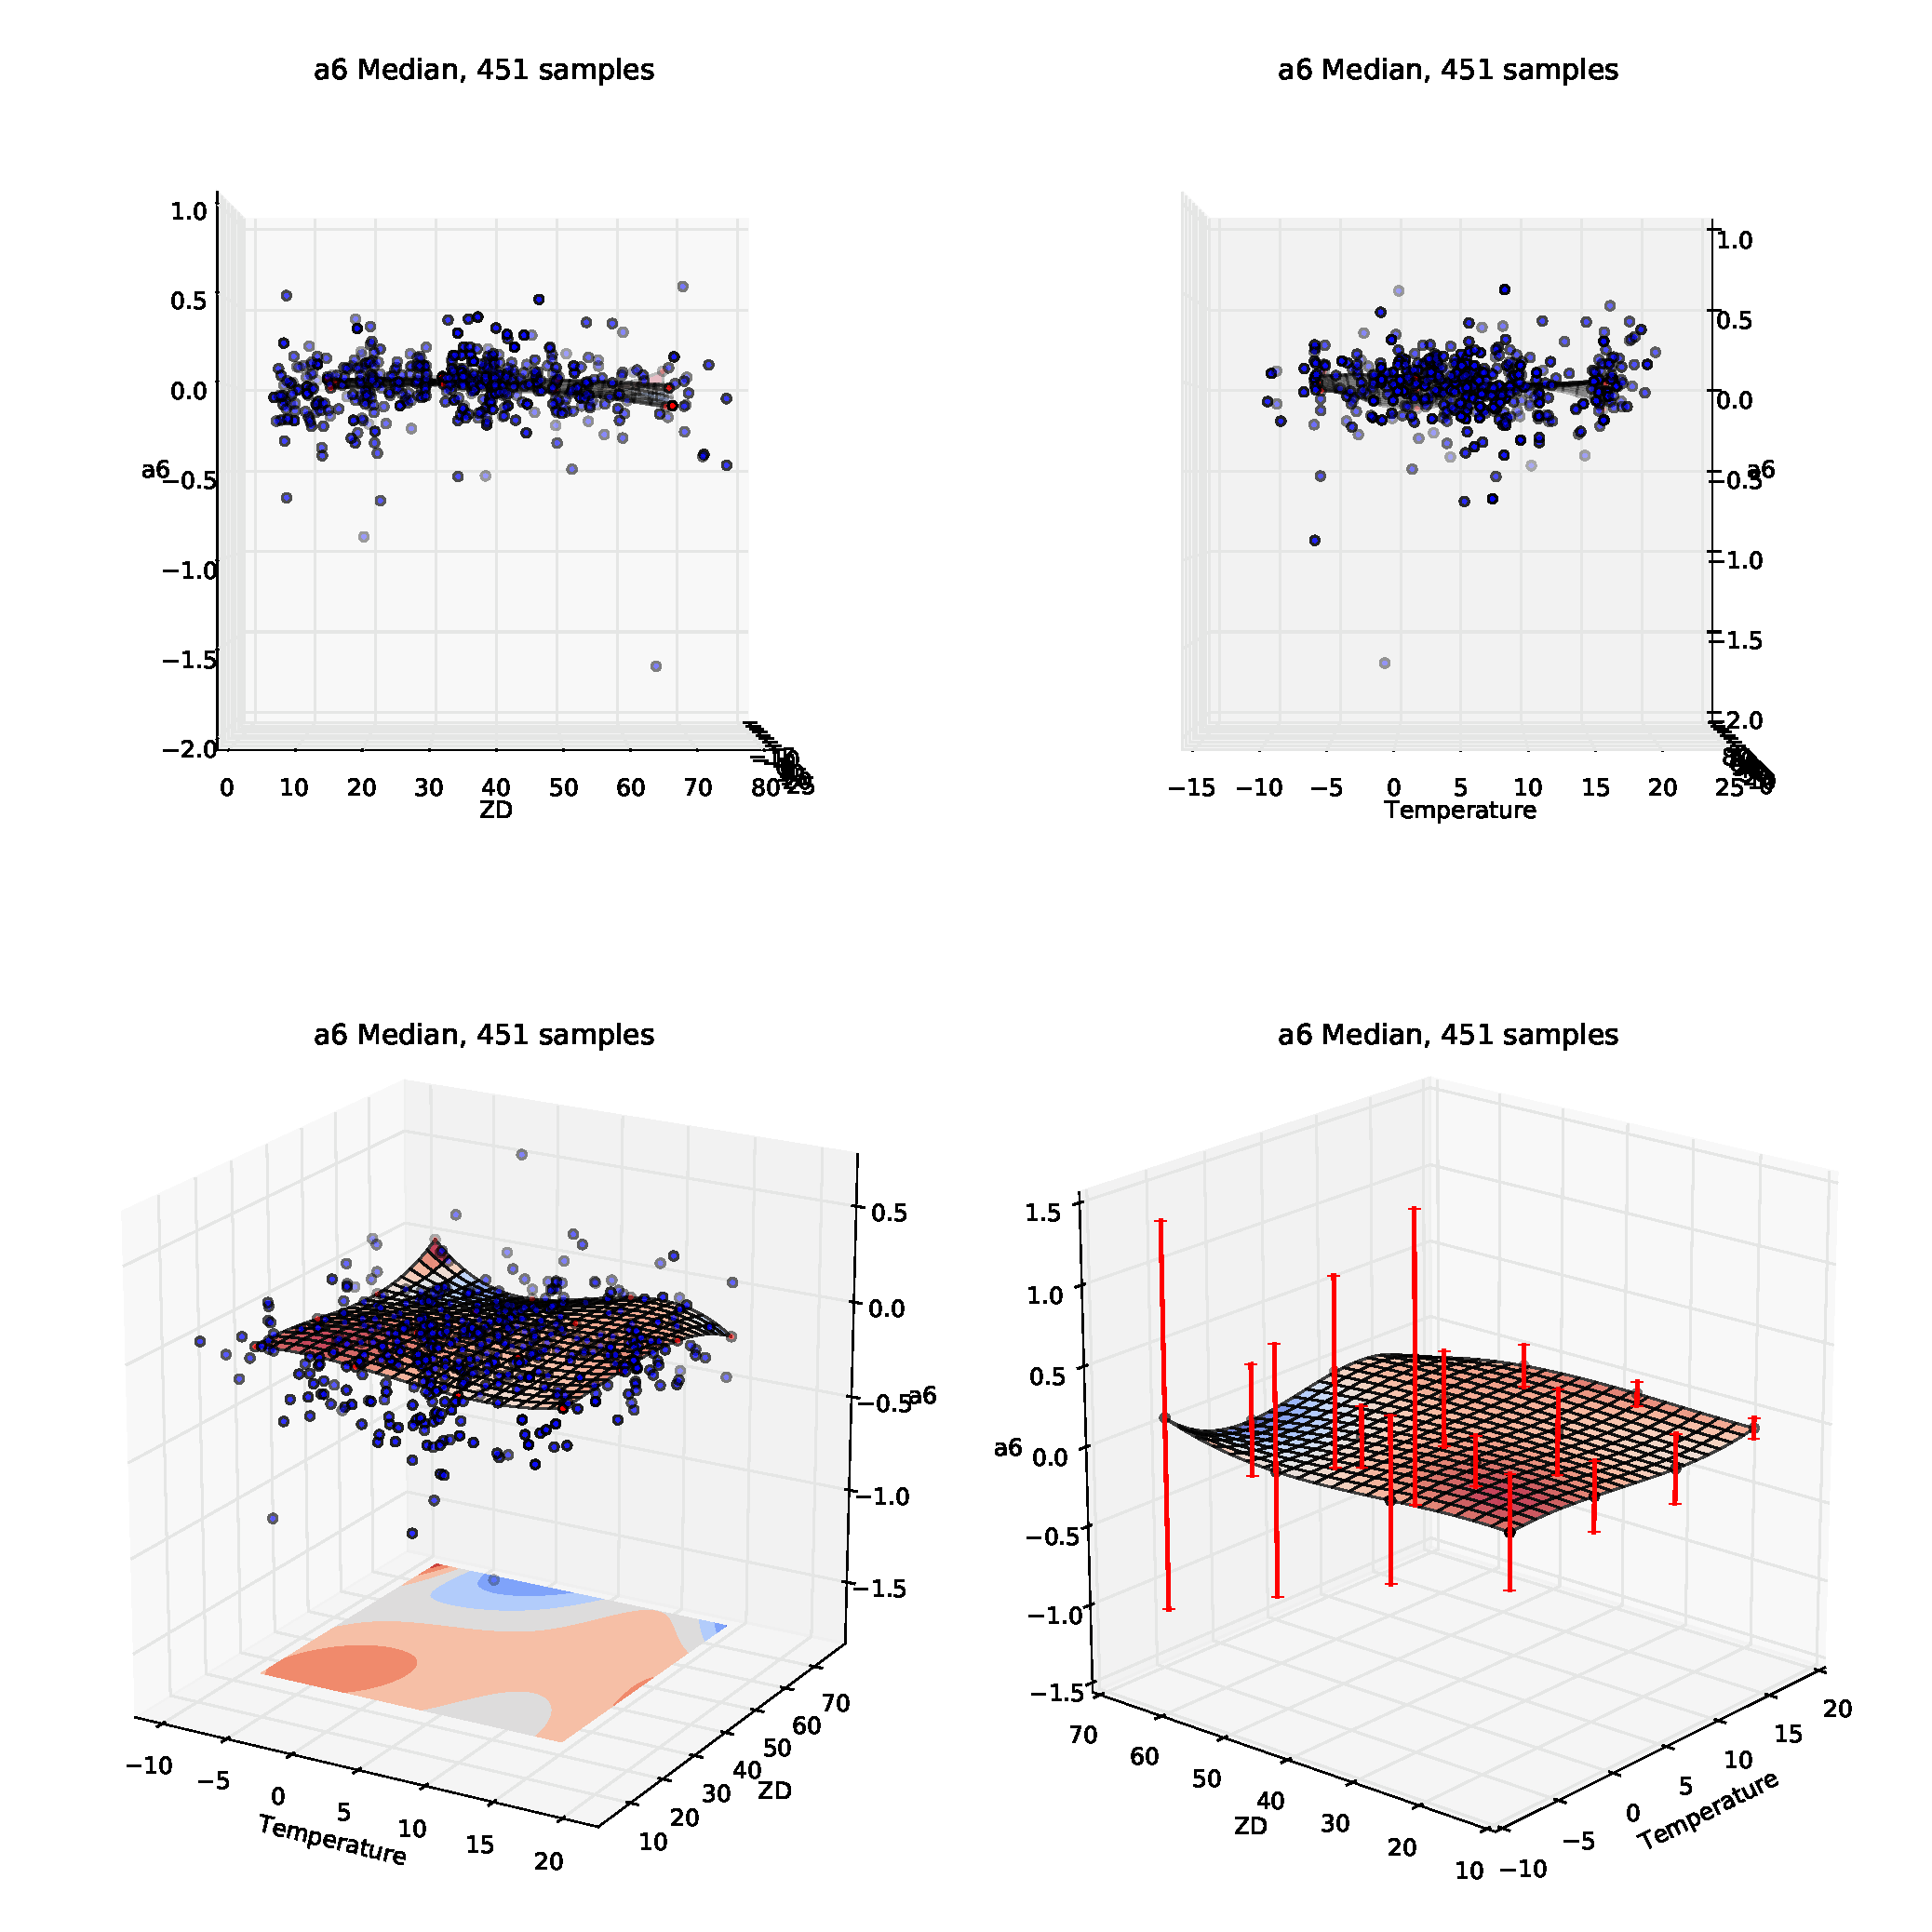
\includegraphics[scale=.48]{psf_surf/a6_med.pdf}
	\caption[Mean Streu- und Flächenplot des PSF-Parameters $A_6$]{Median Streu- und Flächenplot des PSF-Parameters $A_6$}
    \label{psf_surf_a6_med}
\end{figure}

\begin{figure}[H]
	\centering
	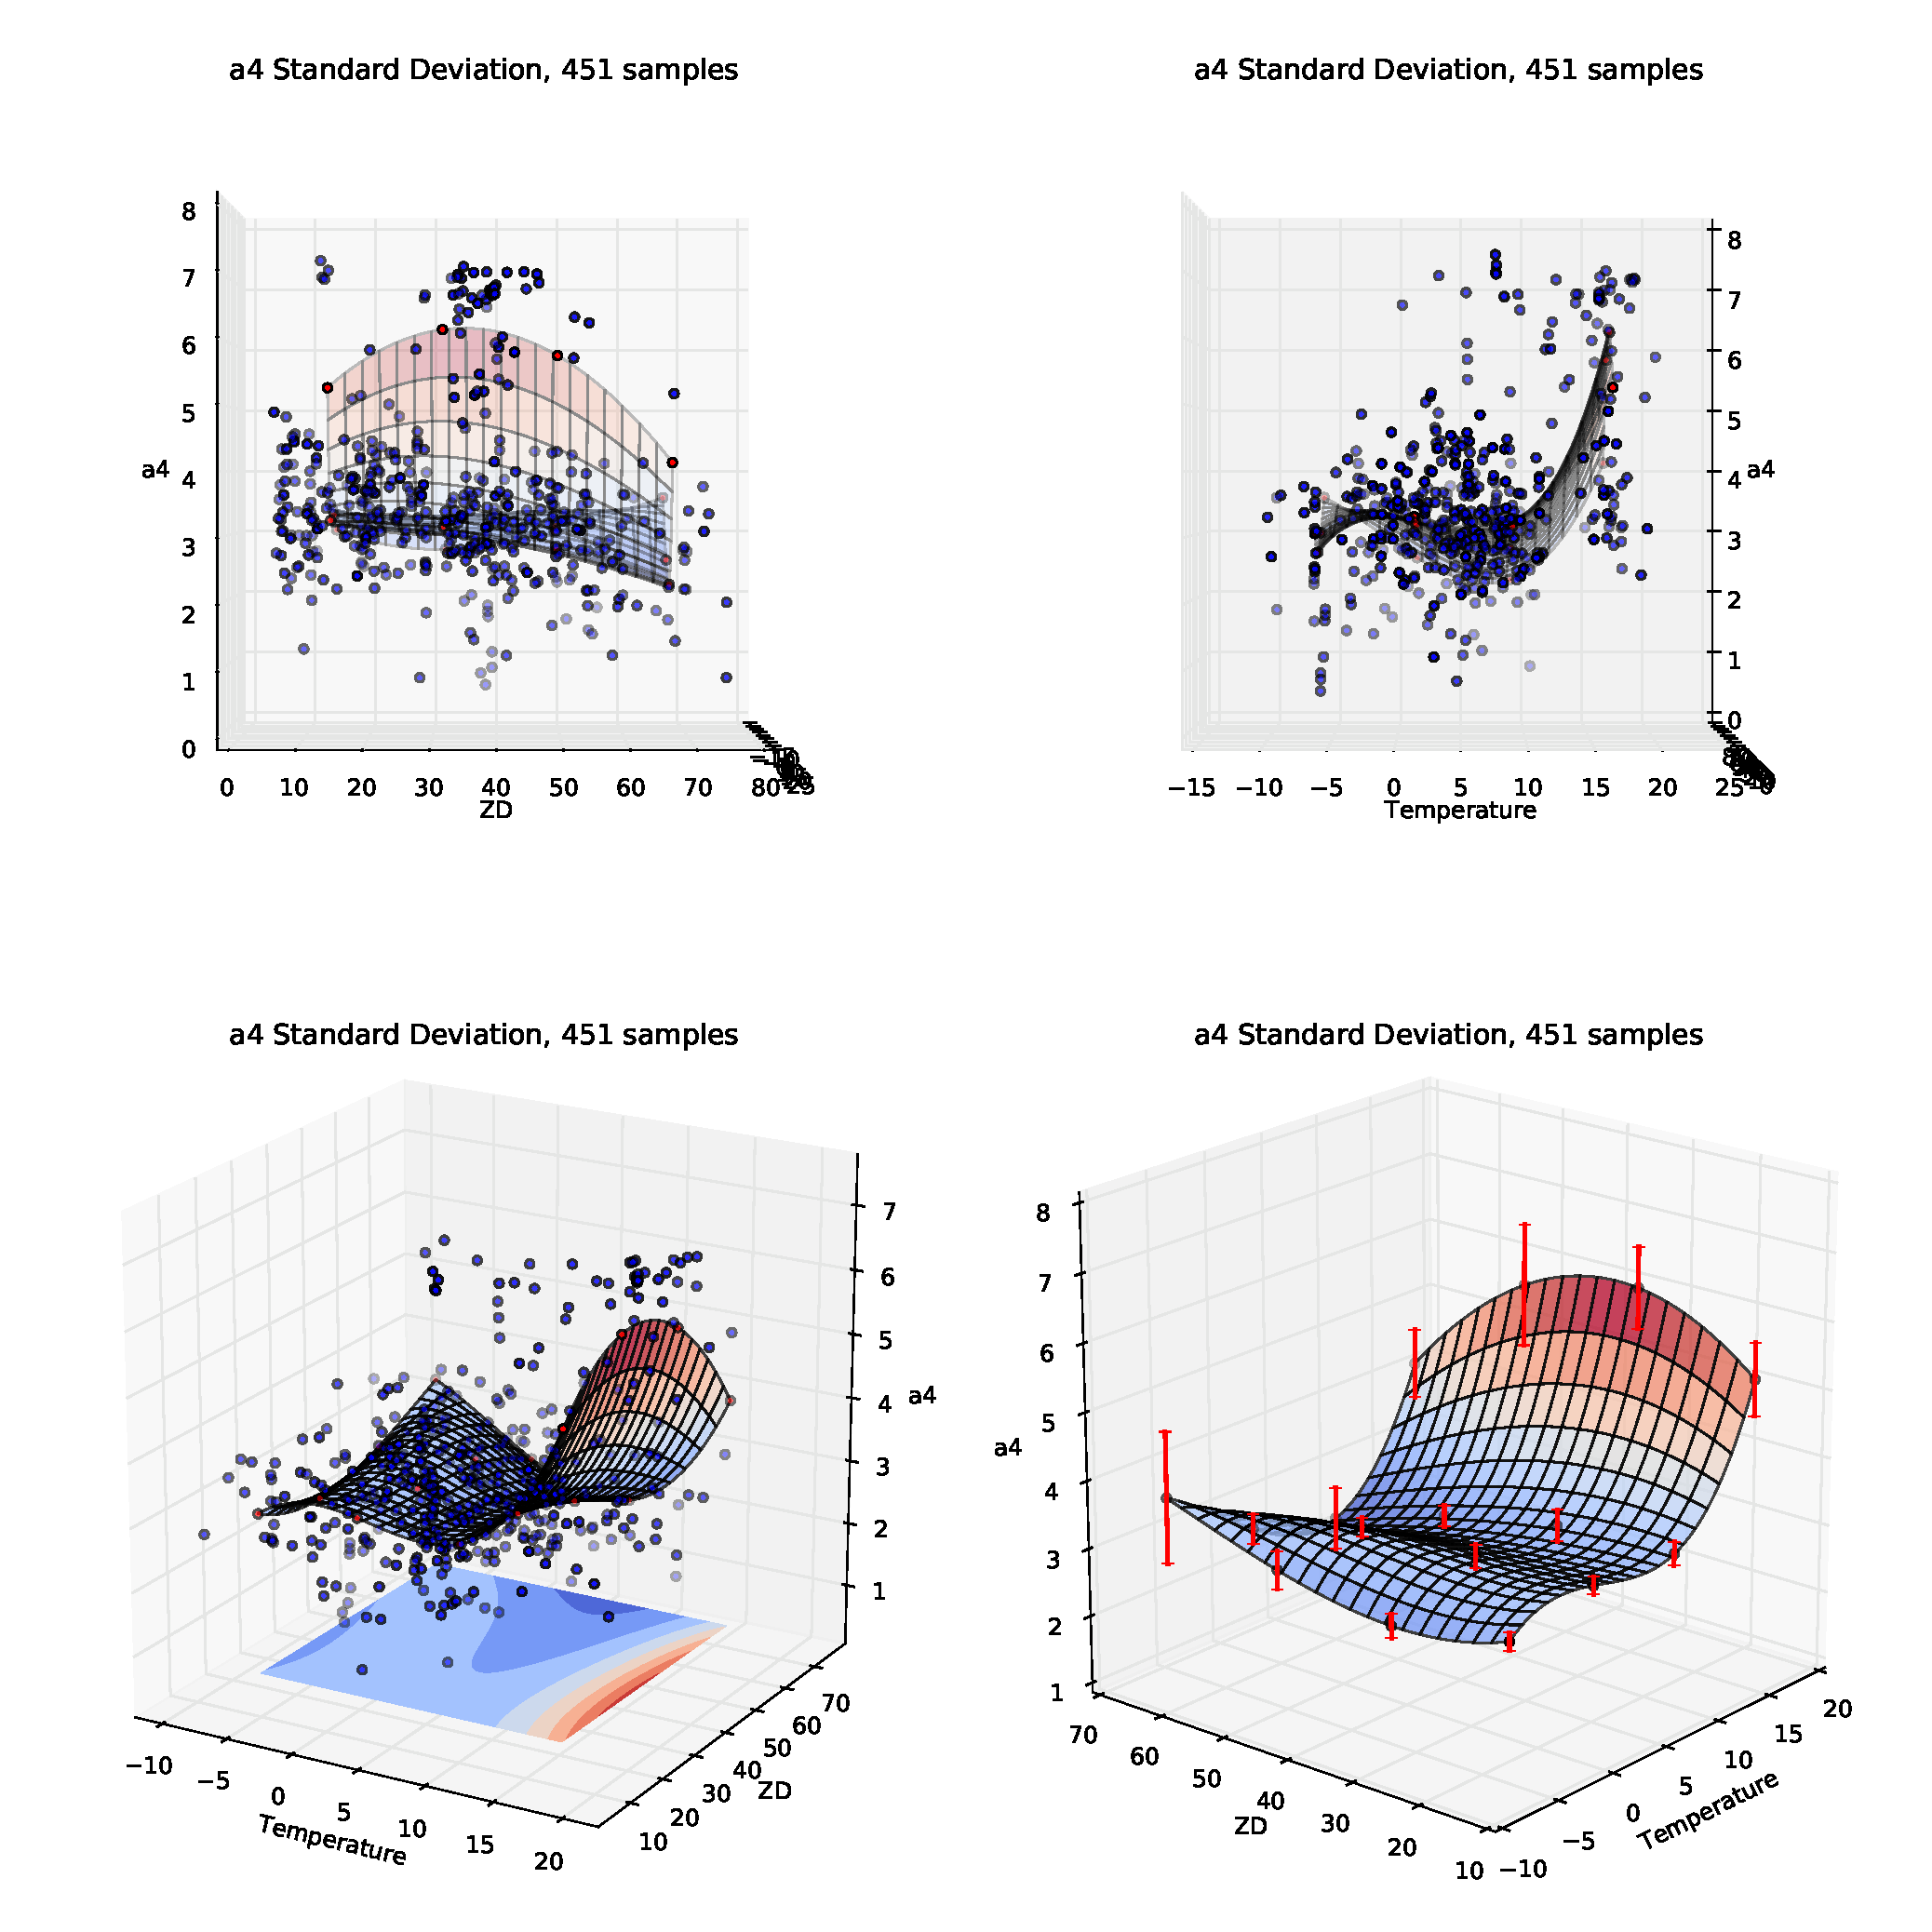
\includegraphics[scale=.48]{psf_surf/a4_std.pdf}
	\caption[Standardabweichung Streu- und Flächenplot des PSF-Parameters $A_4$]{Standardabweichung Streu- und Flächenplot des PSF-Parameters $A_4$}
    \label{psf_surf_a4_std}
\end{figure}
\begin{figure}[H]
	\centering
	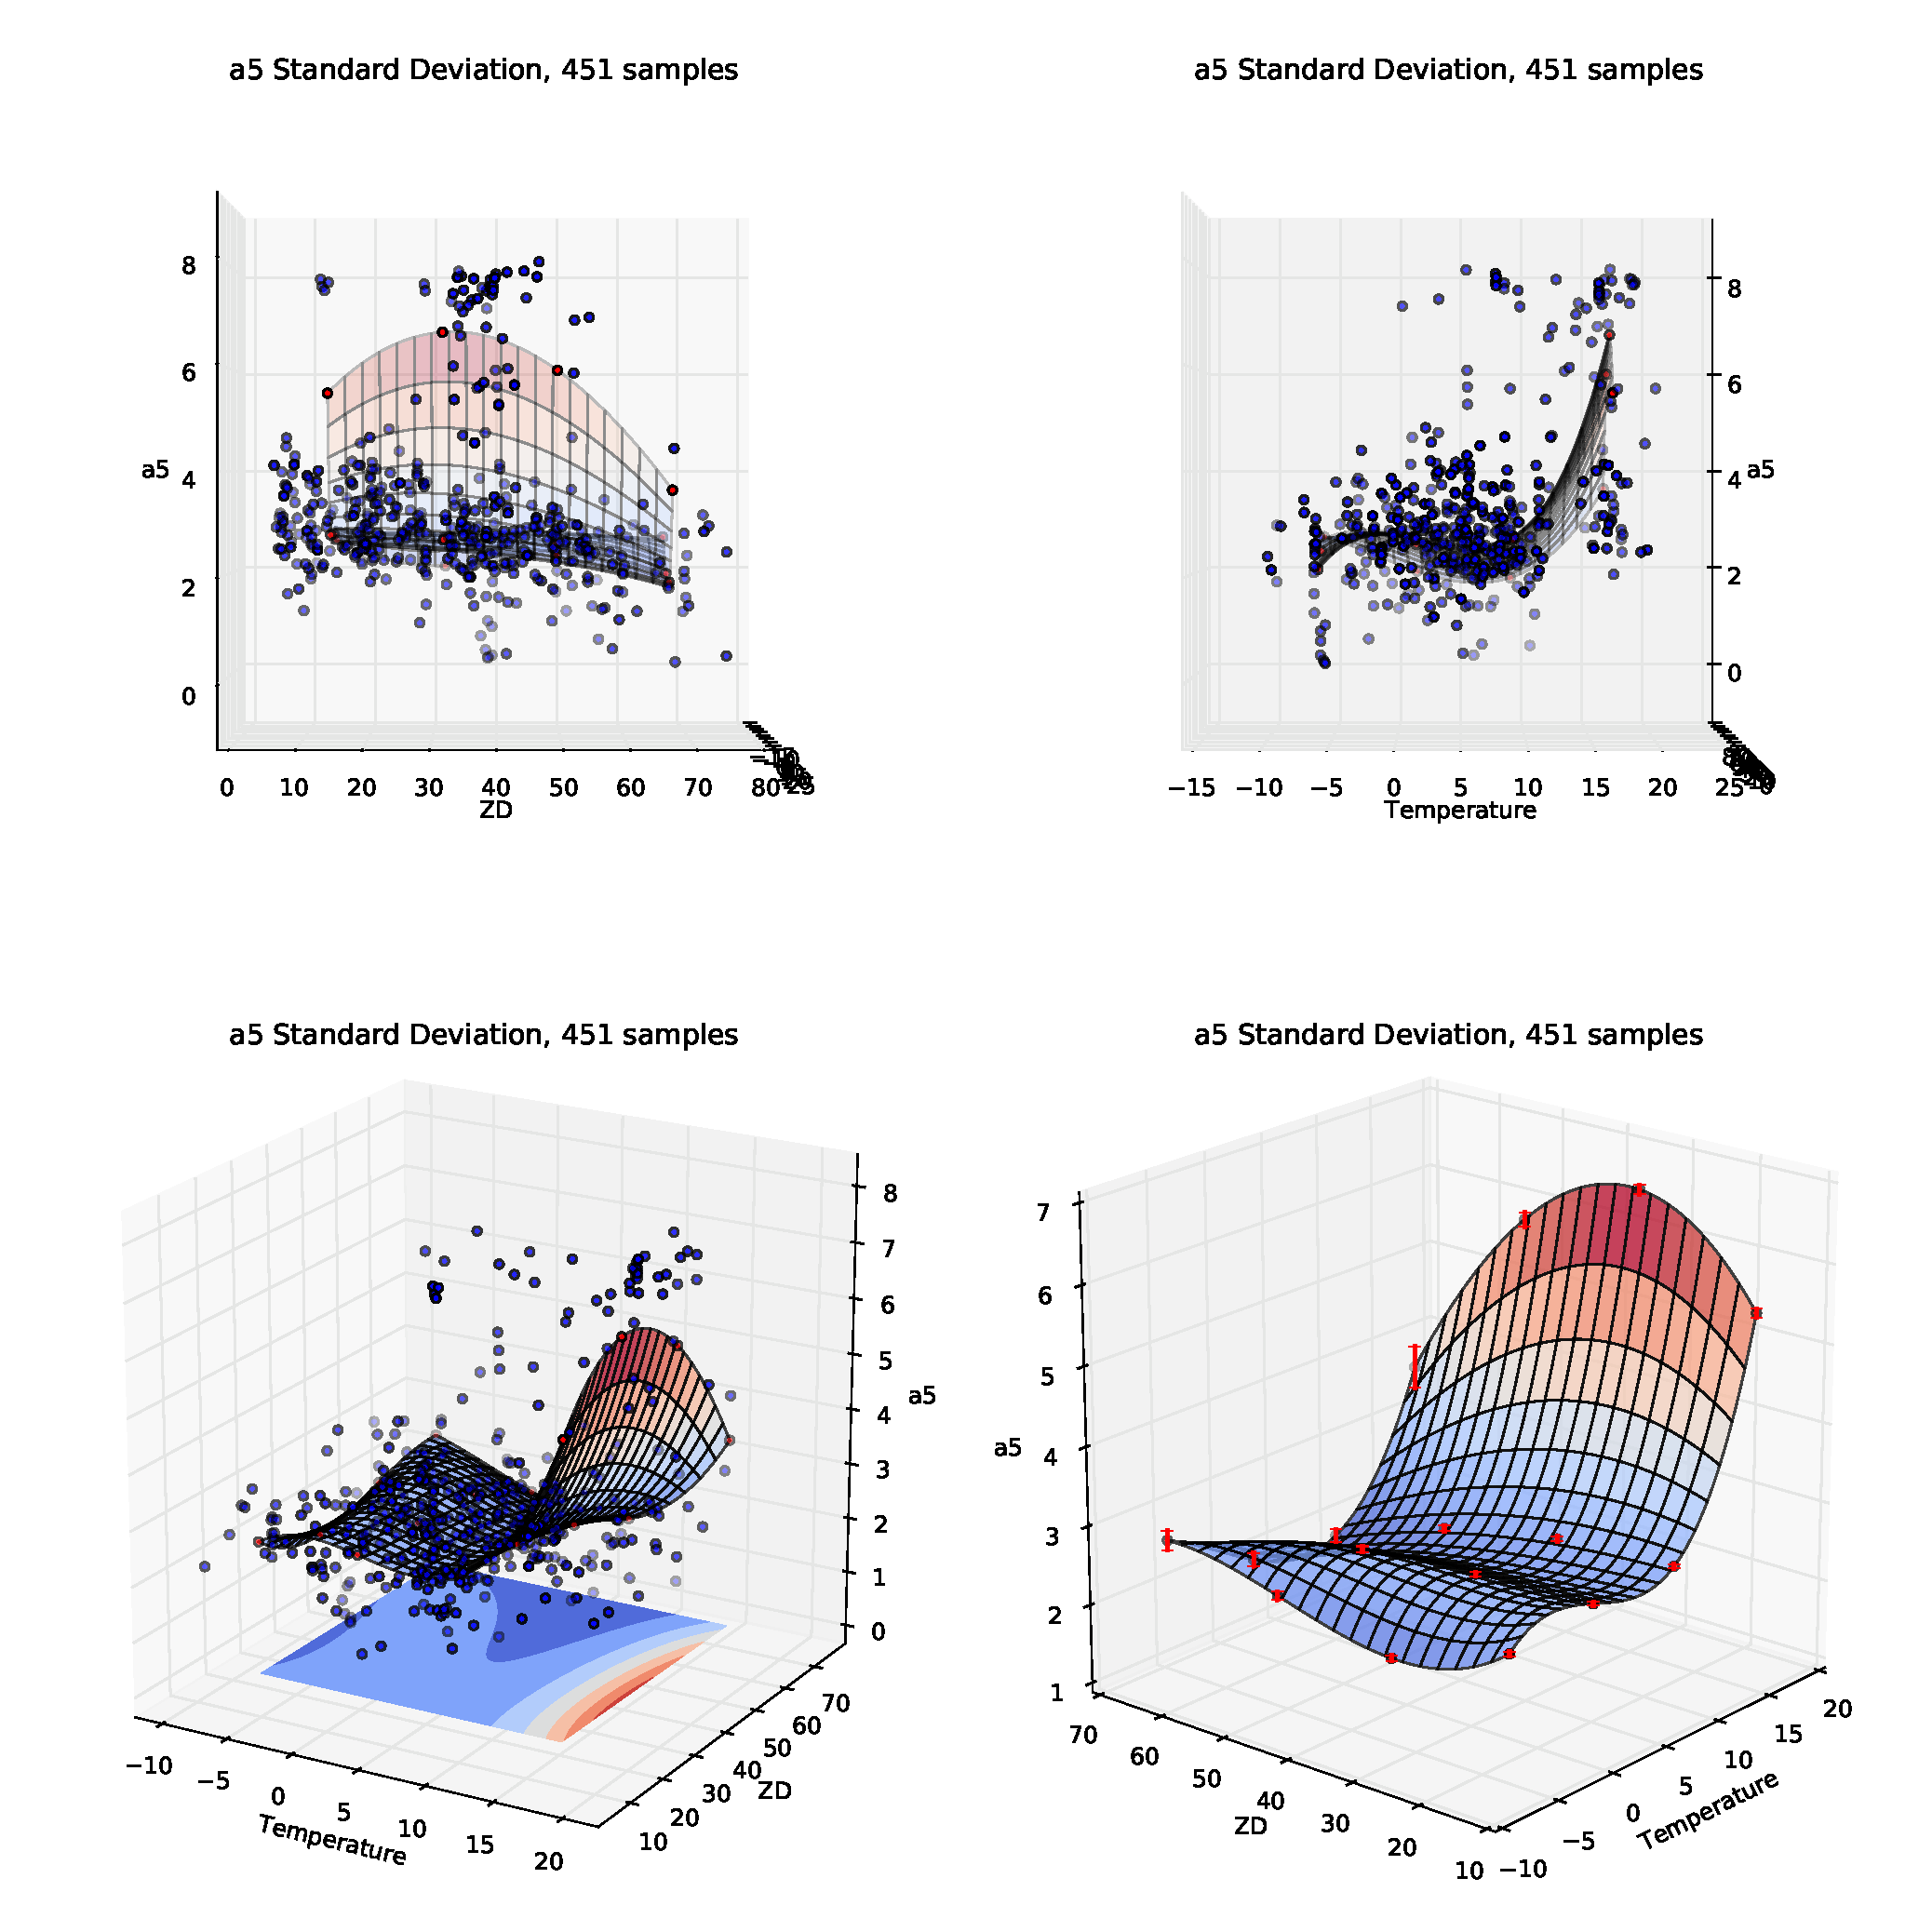
\includegraphics[scale=.48]{psf_surf/a5_std.pdf}
	\caption[Standardabweichung Streu- und Flächenplot des PSF-Parameters $A_5$]{Standardabweichung Streu- und Flächenplot des PSF-Parameters $A_5$}
    \label{psf_surf_a5_std}
\end{figure}
\begin{figure}[H]
	\centering
	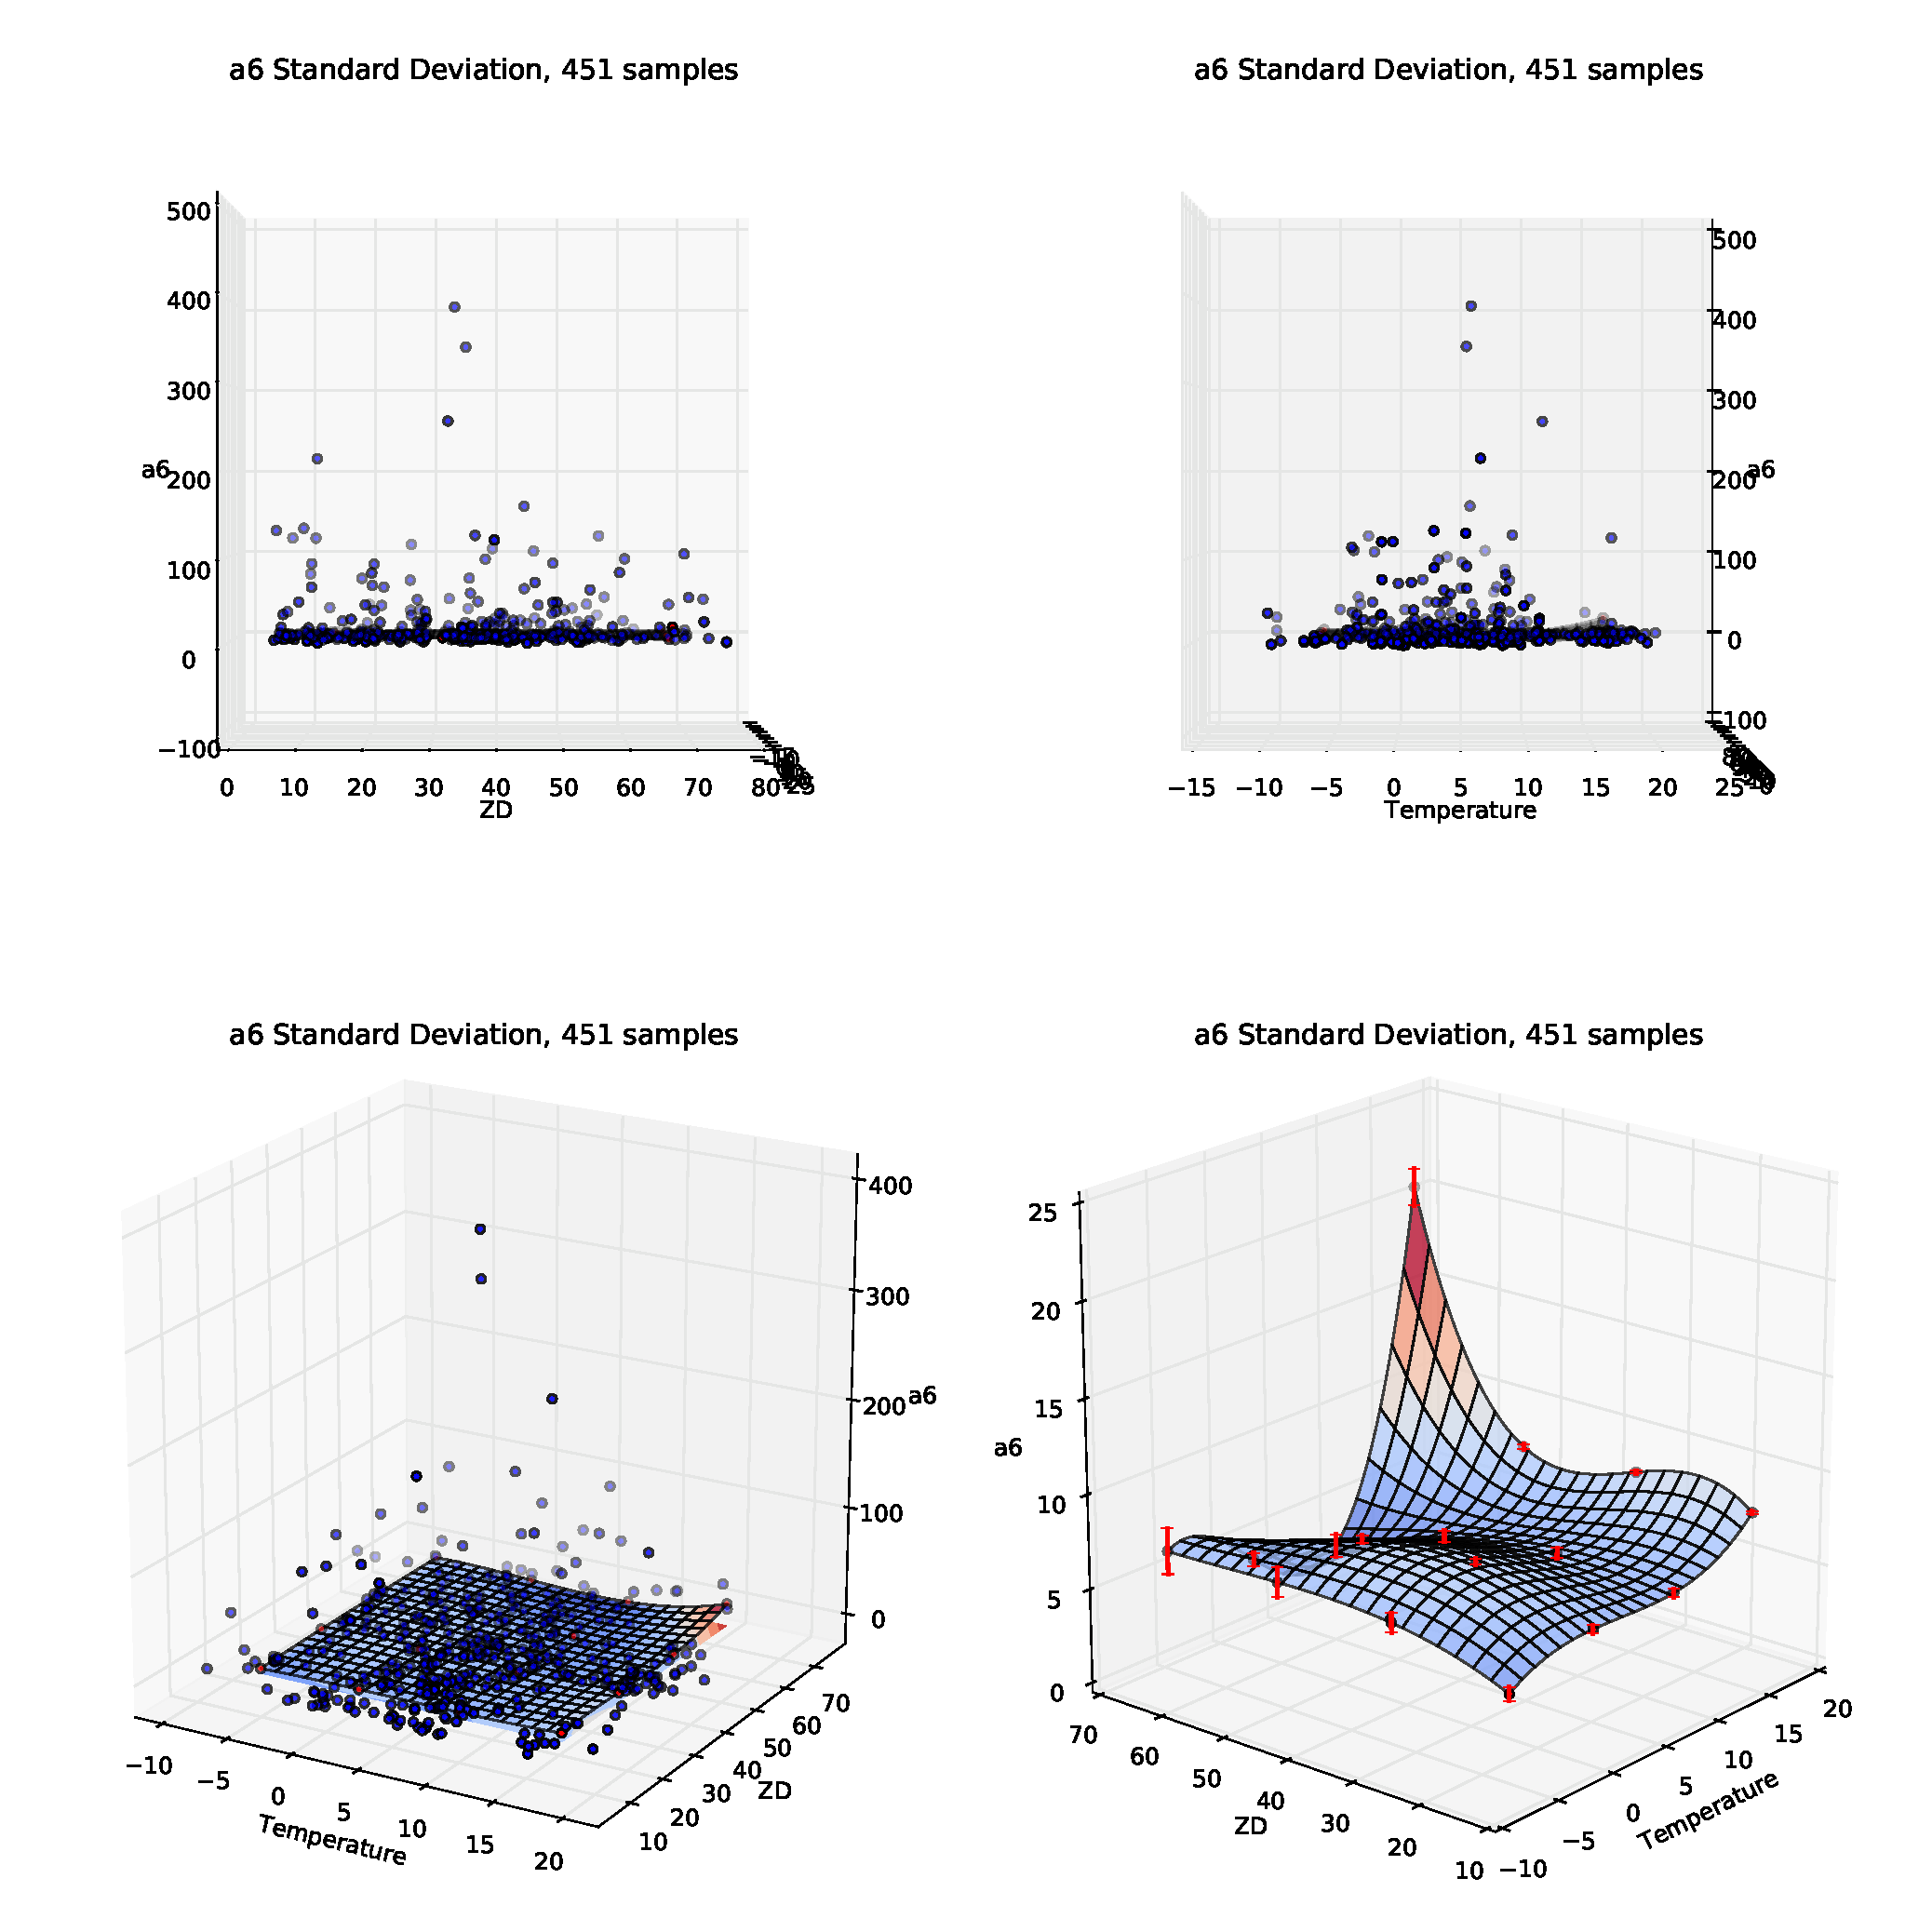
\includegraphics[scale=.48]{psf_surf/a6_std.pdf}
	\caption[Standardabweichung Streu- und Flächenplot des PSF-Parameters $A_6$]{Standardabweichung Streu- und Flächenplot des PSF-Parameters $A_6$}
    \label{psf_surf_a6_std}
\end{figure}

\begin{figure}[H]
	\centering
	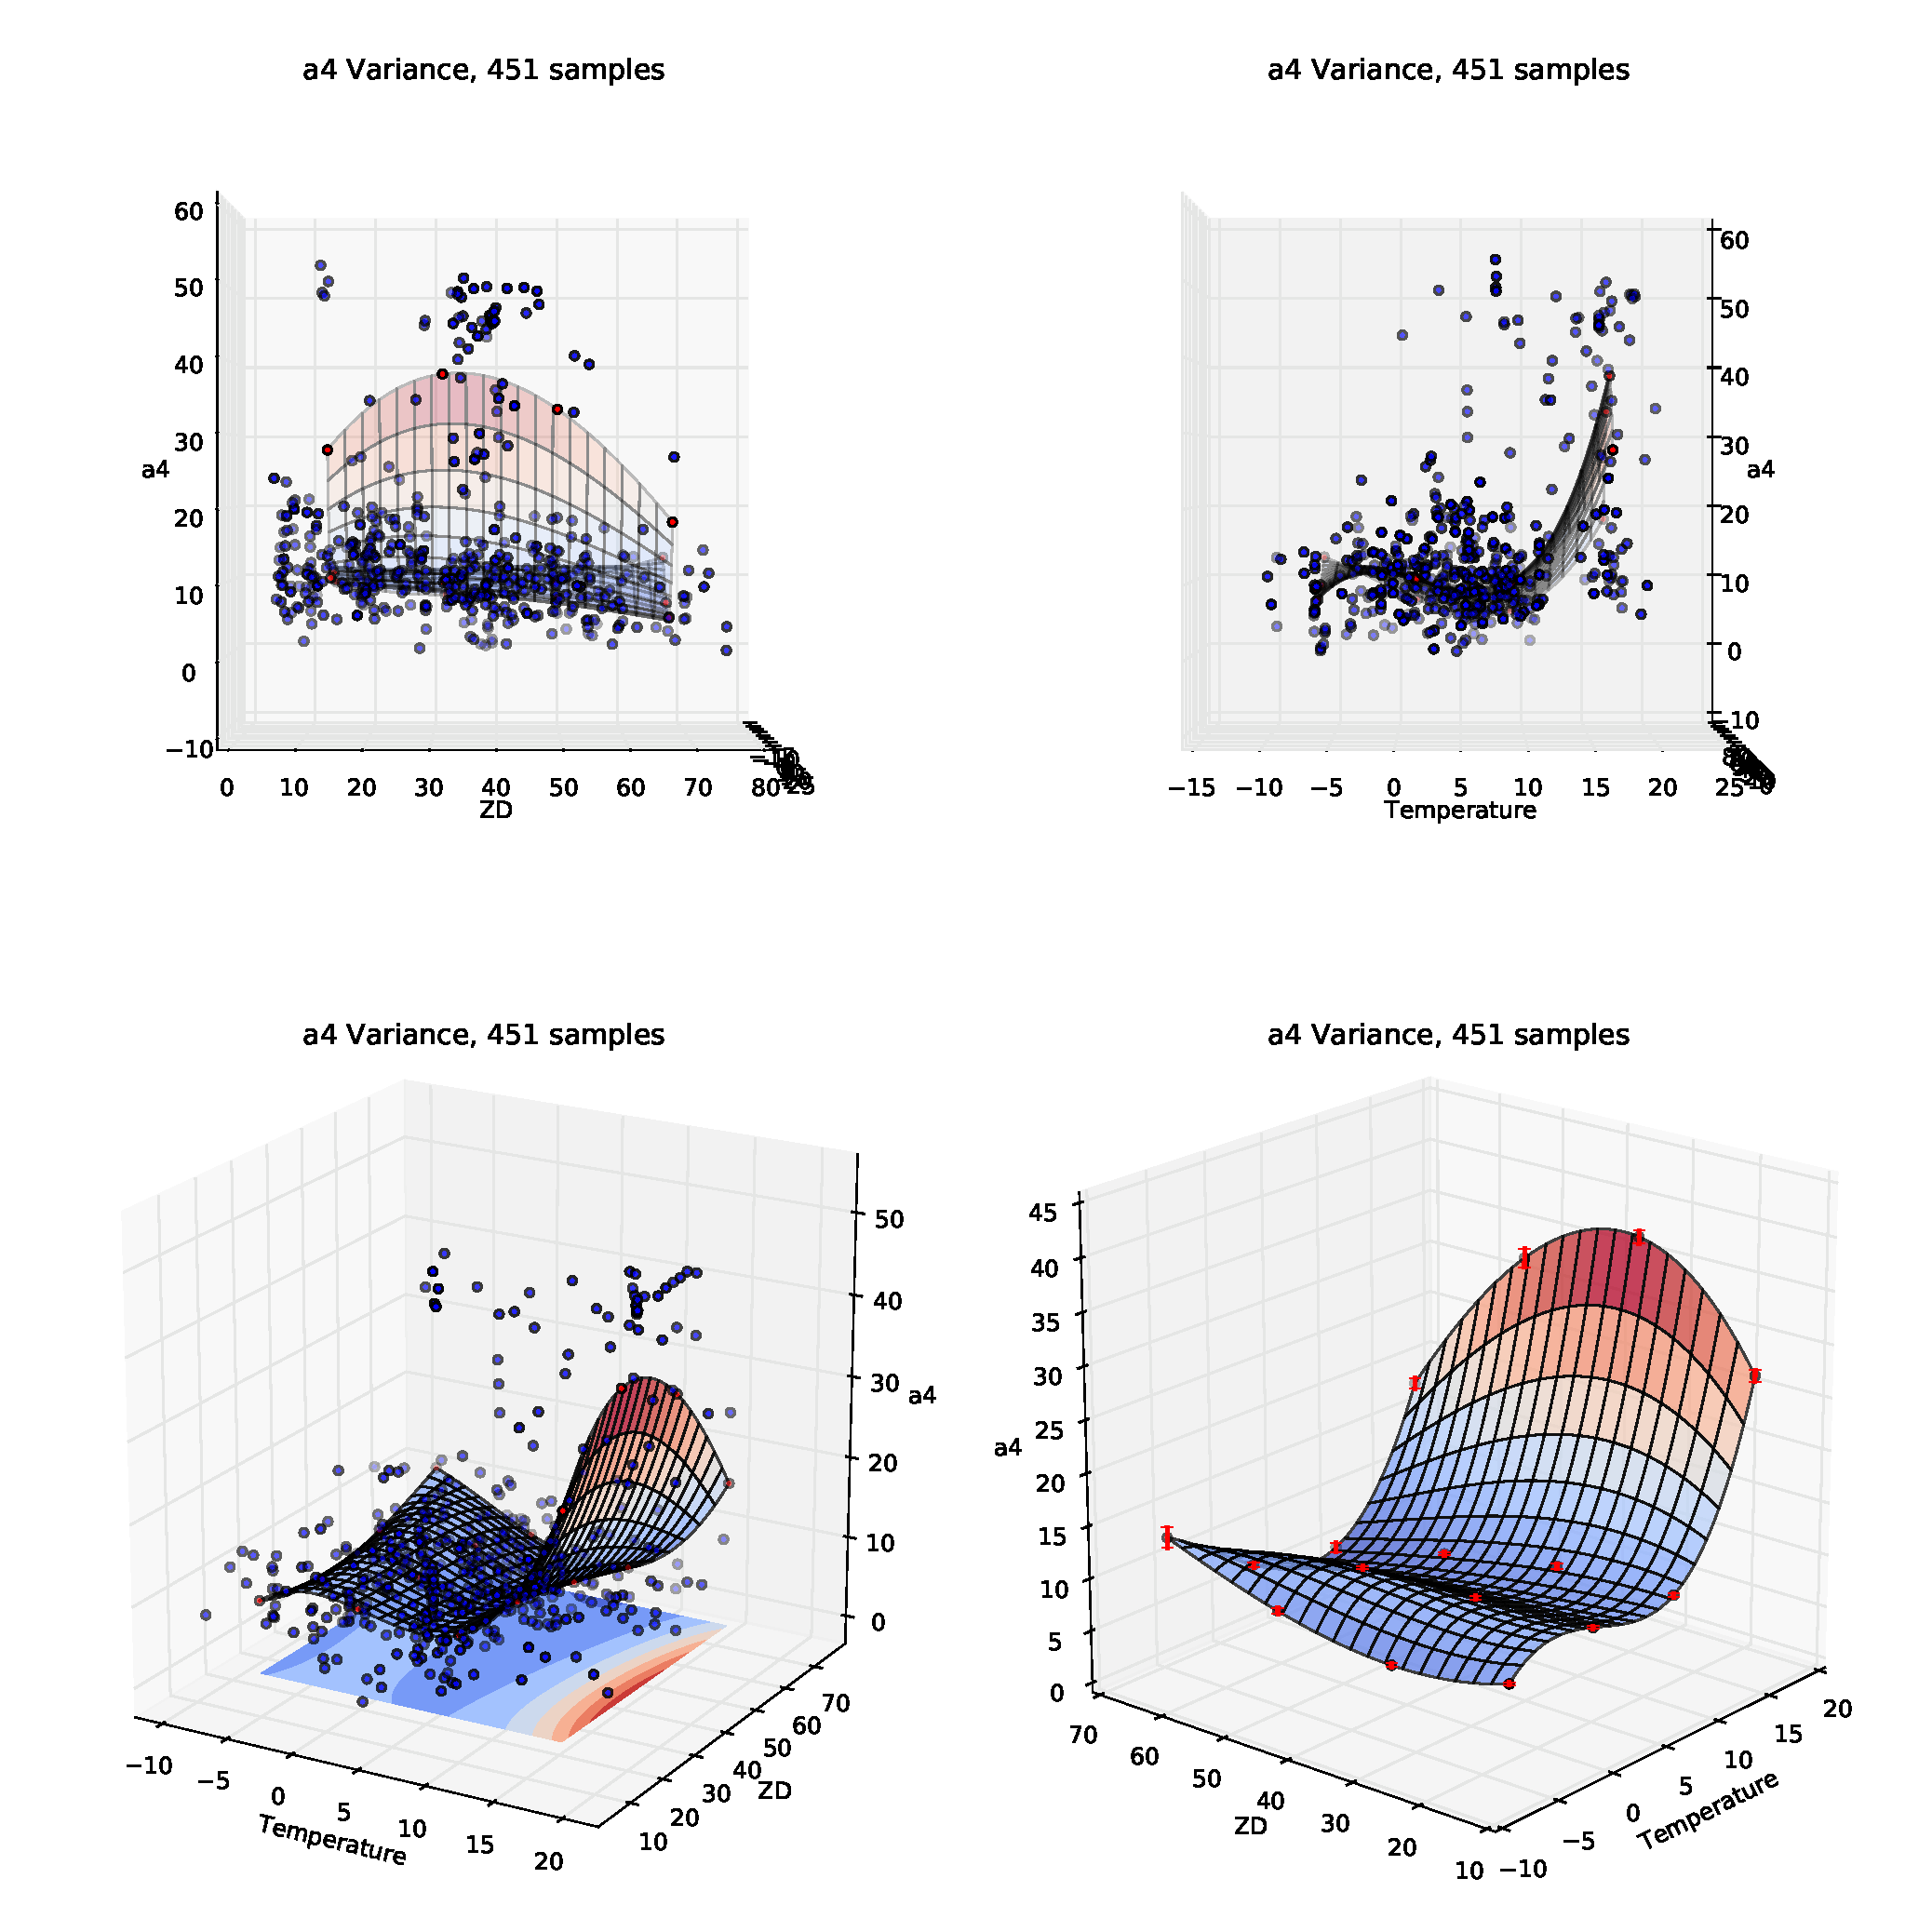
\includegraphics[scale=.48]{psf_surf/a4_var.pdf}
	\caption[Varianz Streu- und Flächenplot des PSF-Parameters $A_4$]{Varianz Streu- und Flächenplot des PSF-Parameters $A_4$}
    \label{psf_surf_a4_var}
\end{figure}
\begin{figure}[H]
	\centering
	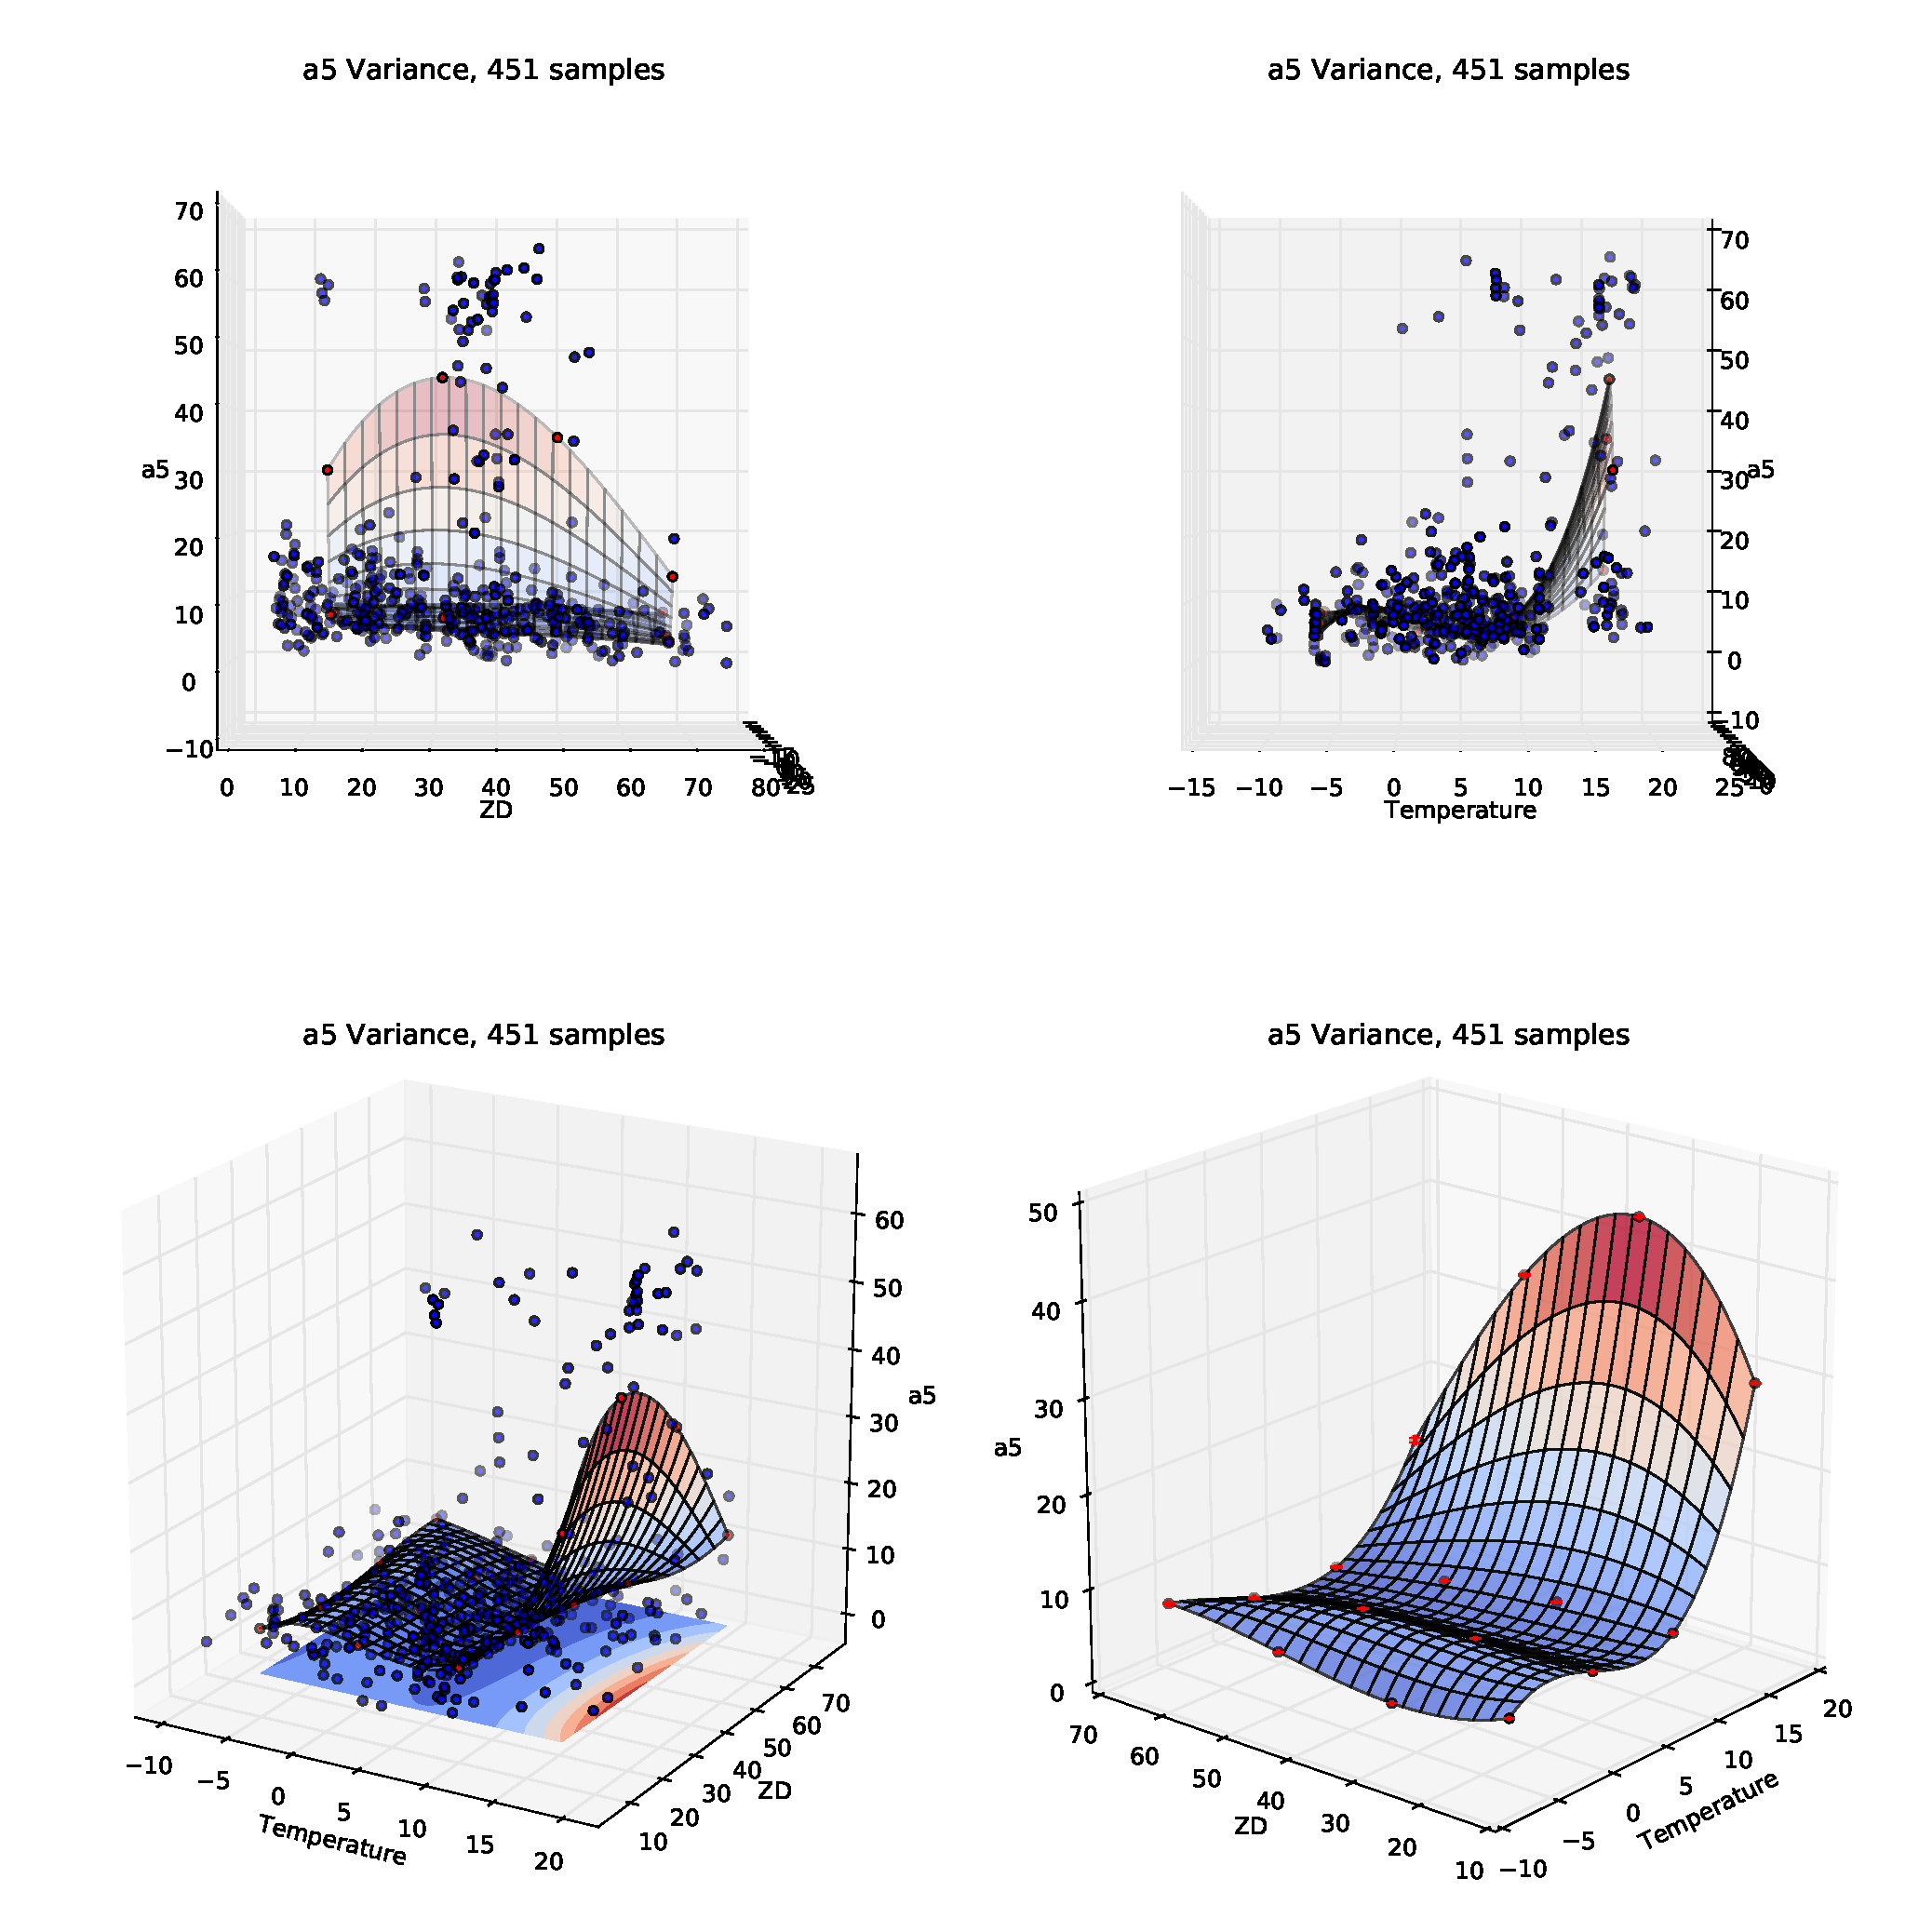
\includegraphics[scale=.48]{psf_surf/a5_var.pdf}
	\caption[Varianz Streu- und Flächenplot des PSF-Parameters $A_5$]{Varianz Streu- und Flächenplot des PSF-Parameters $A_5$}
    \label{psf_surf_a5_var}
\end{figure}
\begin{figure}[H]
	\centering
	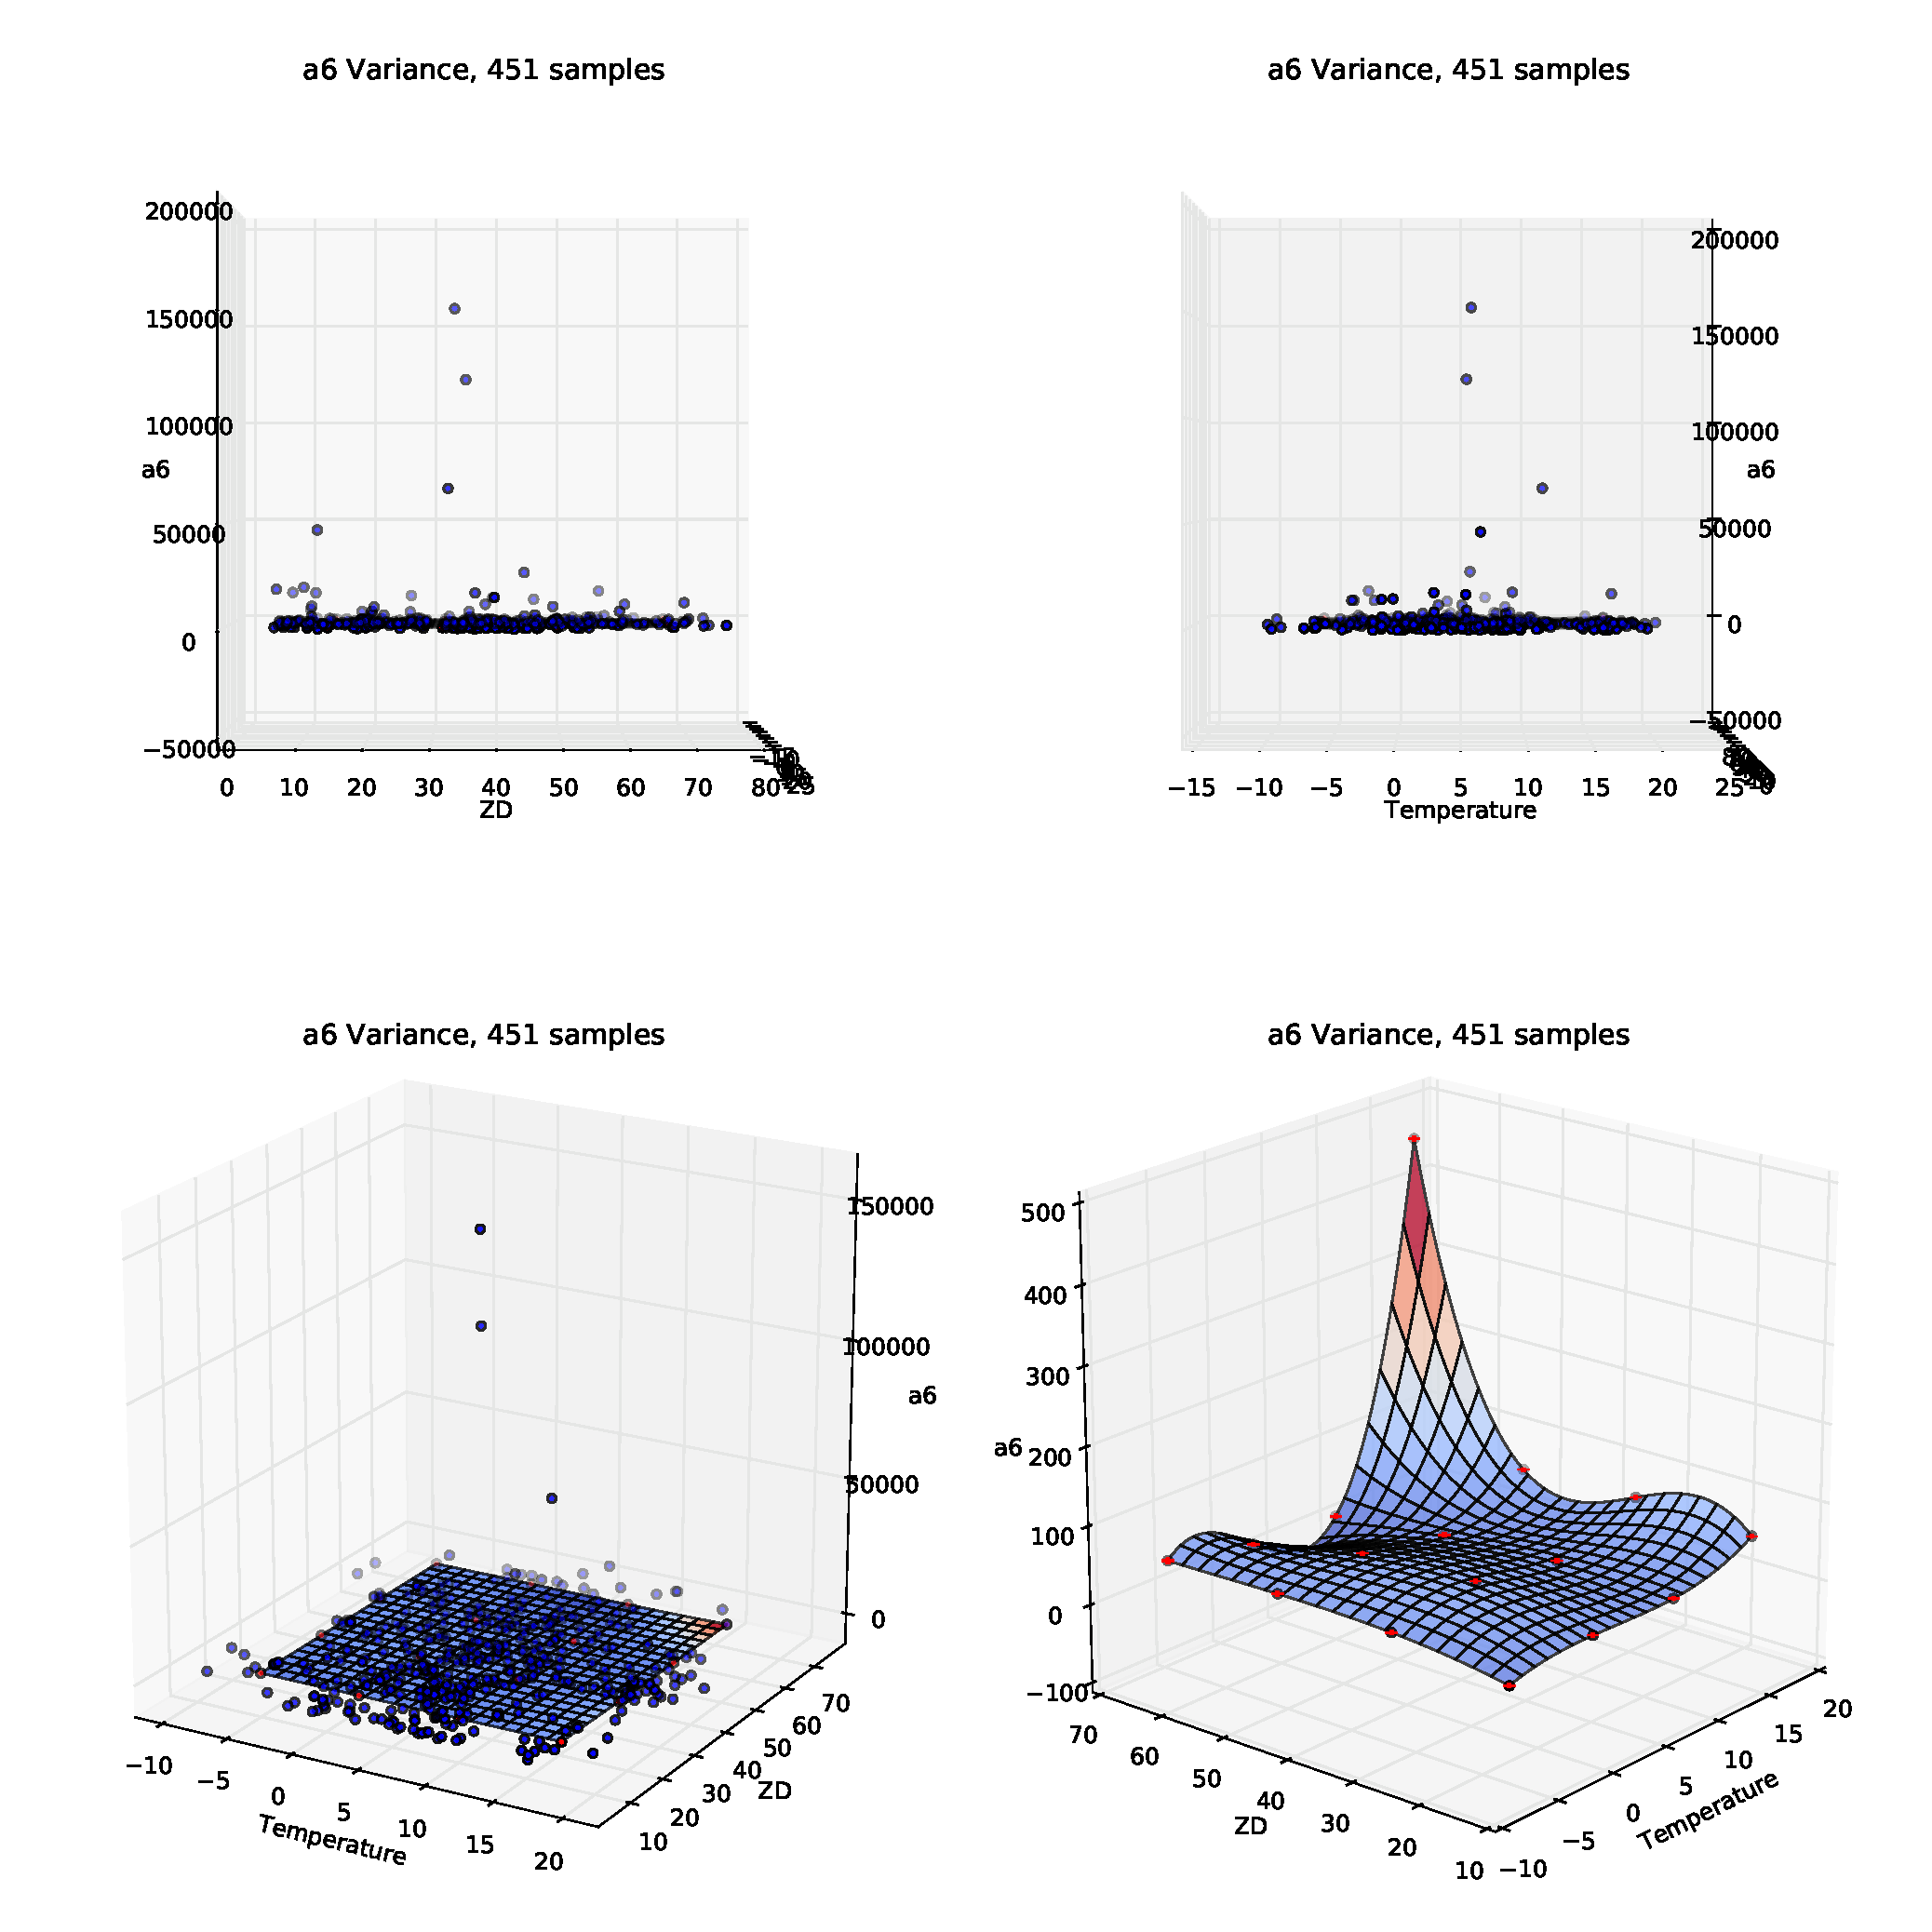
\includegraphics[scale=.48]{psf_surf/a6_var.pdf}
	\caption[Varianz Streu- und Flächenplot des PSF-Parameters $A_6$]{Varianz Streu- und Flächenplot des PSF-Parameters $A_6$}
    \label{psf_surf_a6_var}
\end{figure}

\section{TSI-Verteilungen}
Die TSI-Parameter sind zu zahlreich um alle 124 nicht-statischen diskreten Verteilungsfunktionen an dieser Stelle aufzuzeigen. Stattdessen können sie bei Bedarf online nachgeschlagen oder heruntergeladen werden.
\begin{mdframed}[style=emphasis]
	\centering
	\url{http://homepages.physik.uni-muenchen.de/~Jean.Elsner/focus-series/plots/}
\end{mdframed}
\vfill\,

\section{Sekundärspiegel Temperatur- und Elevationsabhängigkeit}

\begin{figure}[H]
	\centering
	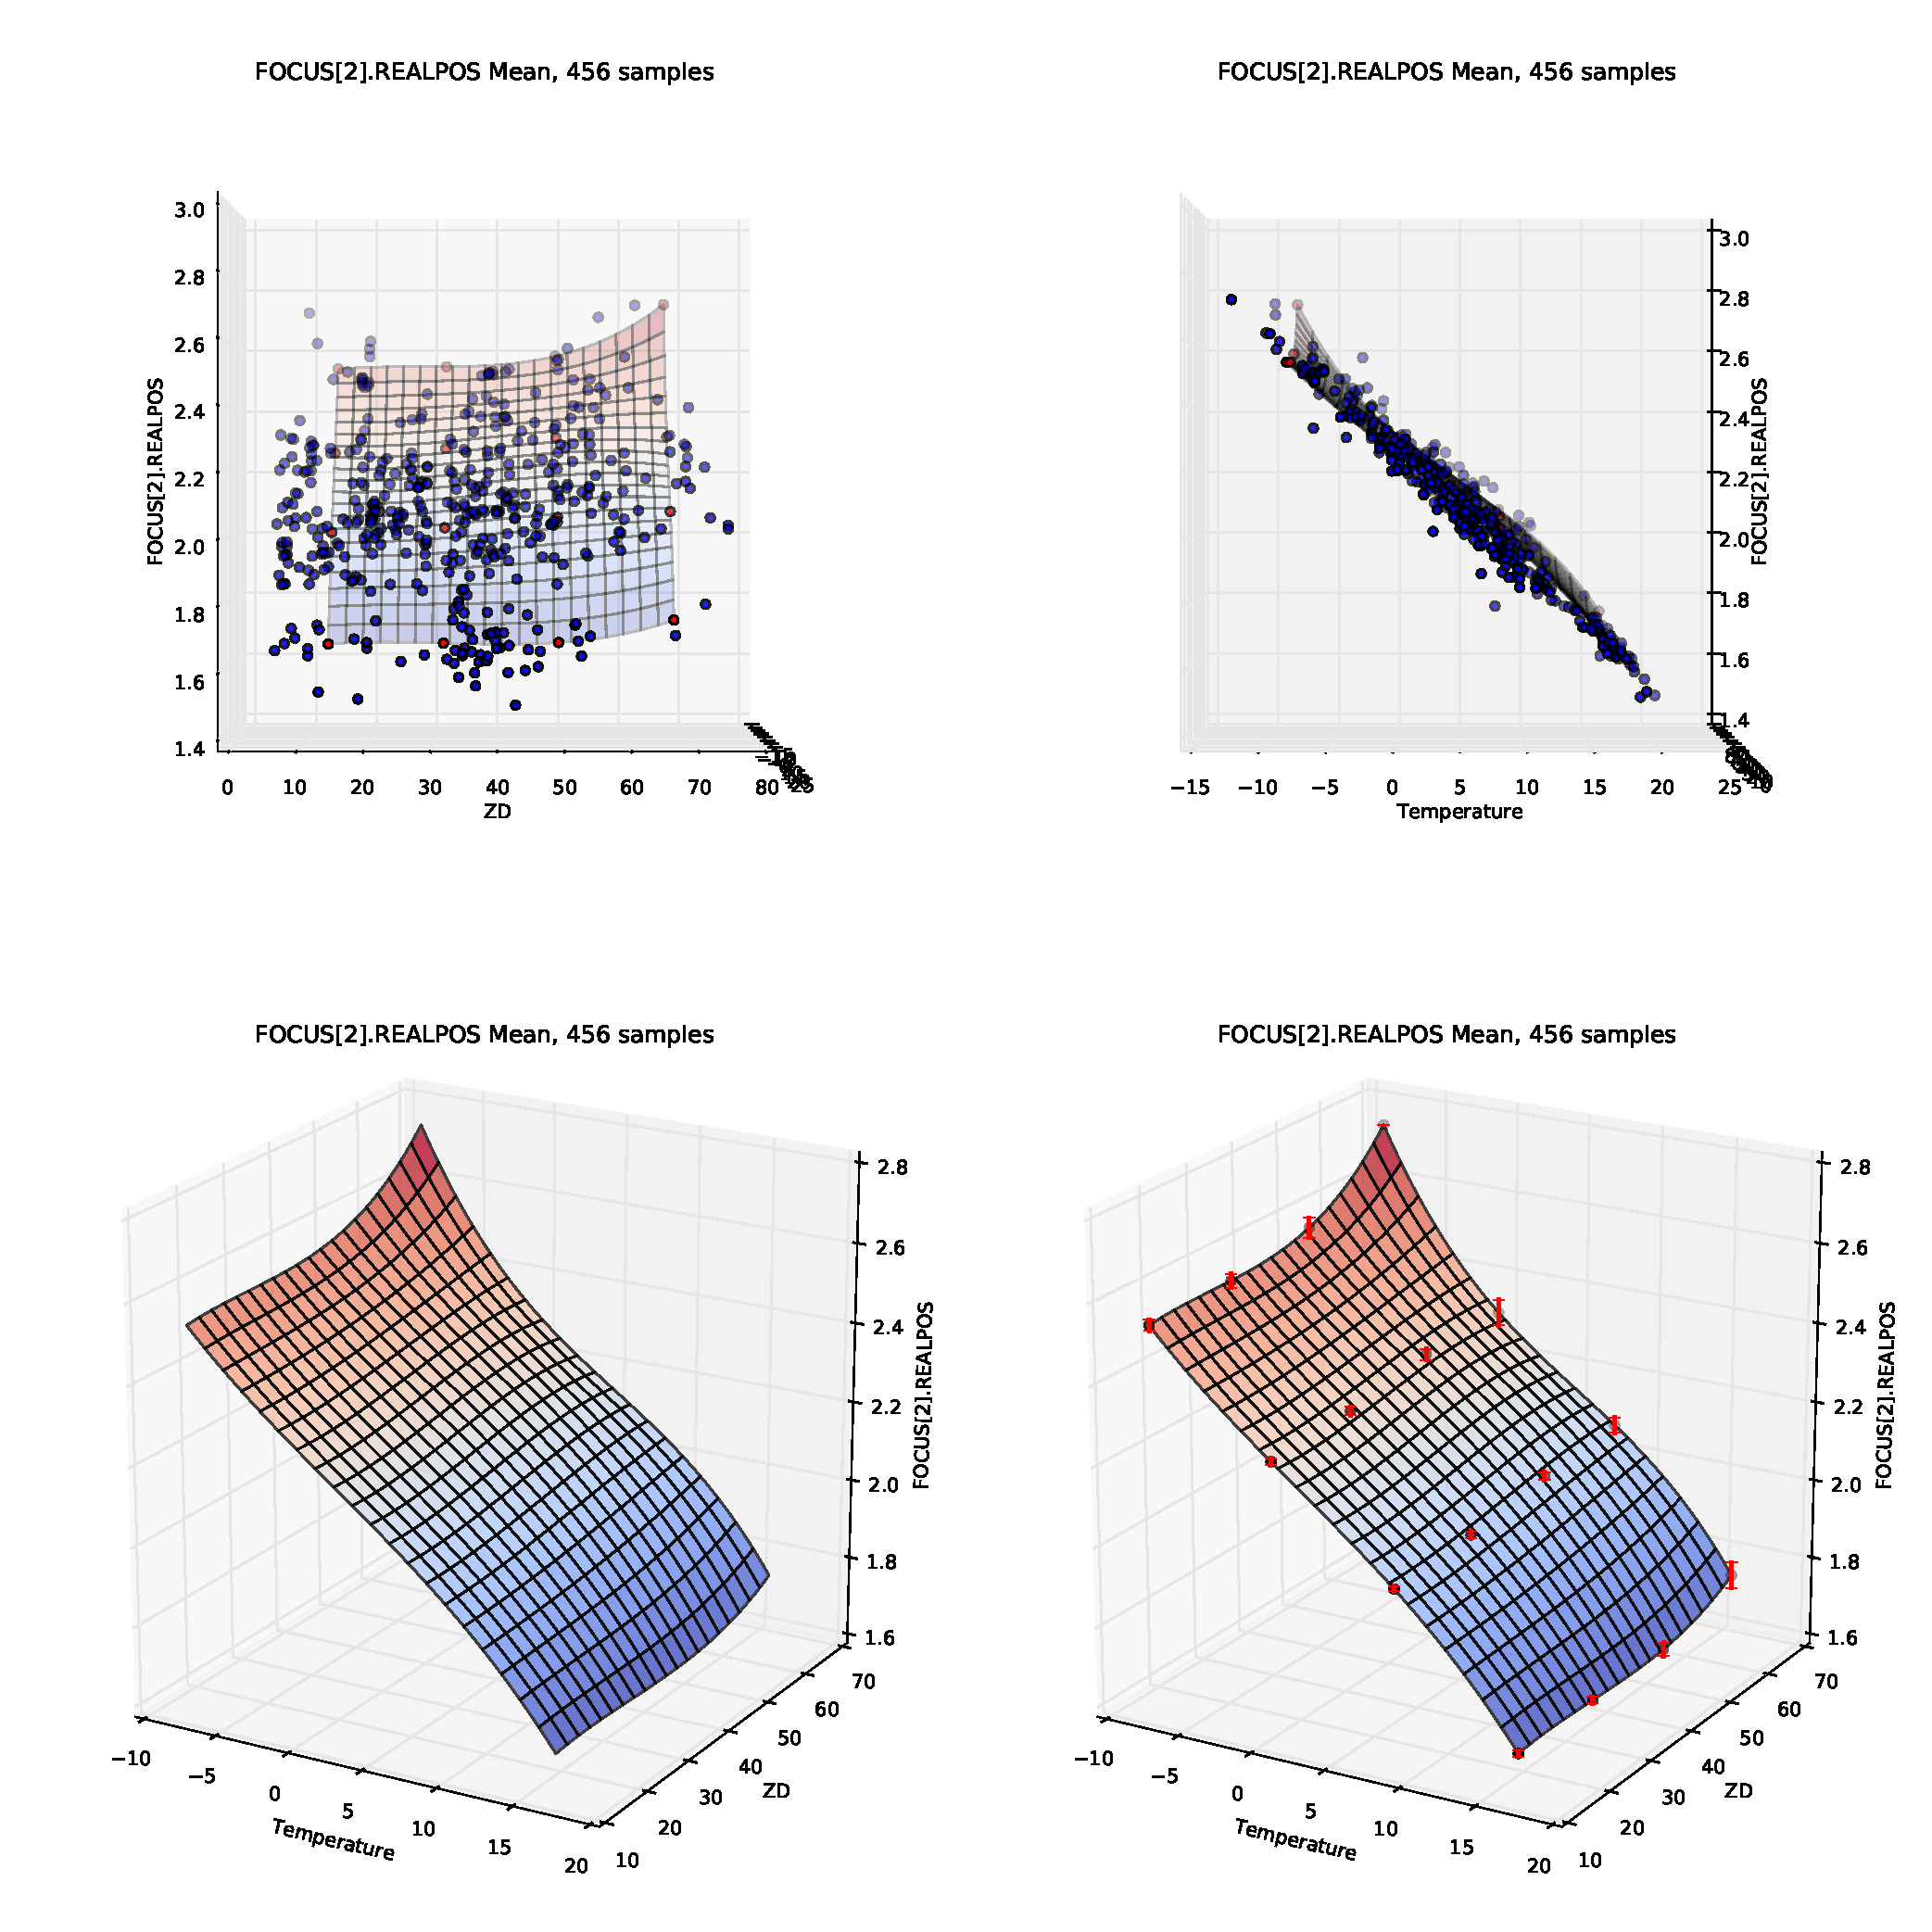
\includegraphics[scale=.44]{tsi_surf/POSITION_INSTRUMENTAL_FOCUS_2__REALPOS_mean.pdf}
	\caption[Mean Streu- und Flächenplot des Sekundärspiegels]{Mean Streu- und Flächenplot des Sekundärspiegels}
    \label{foc_mean}
\end{figure}
\begin{figure}[H]
	\centering
	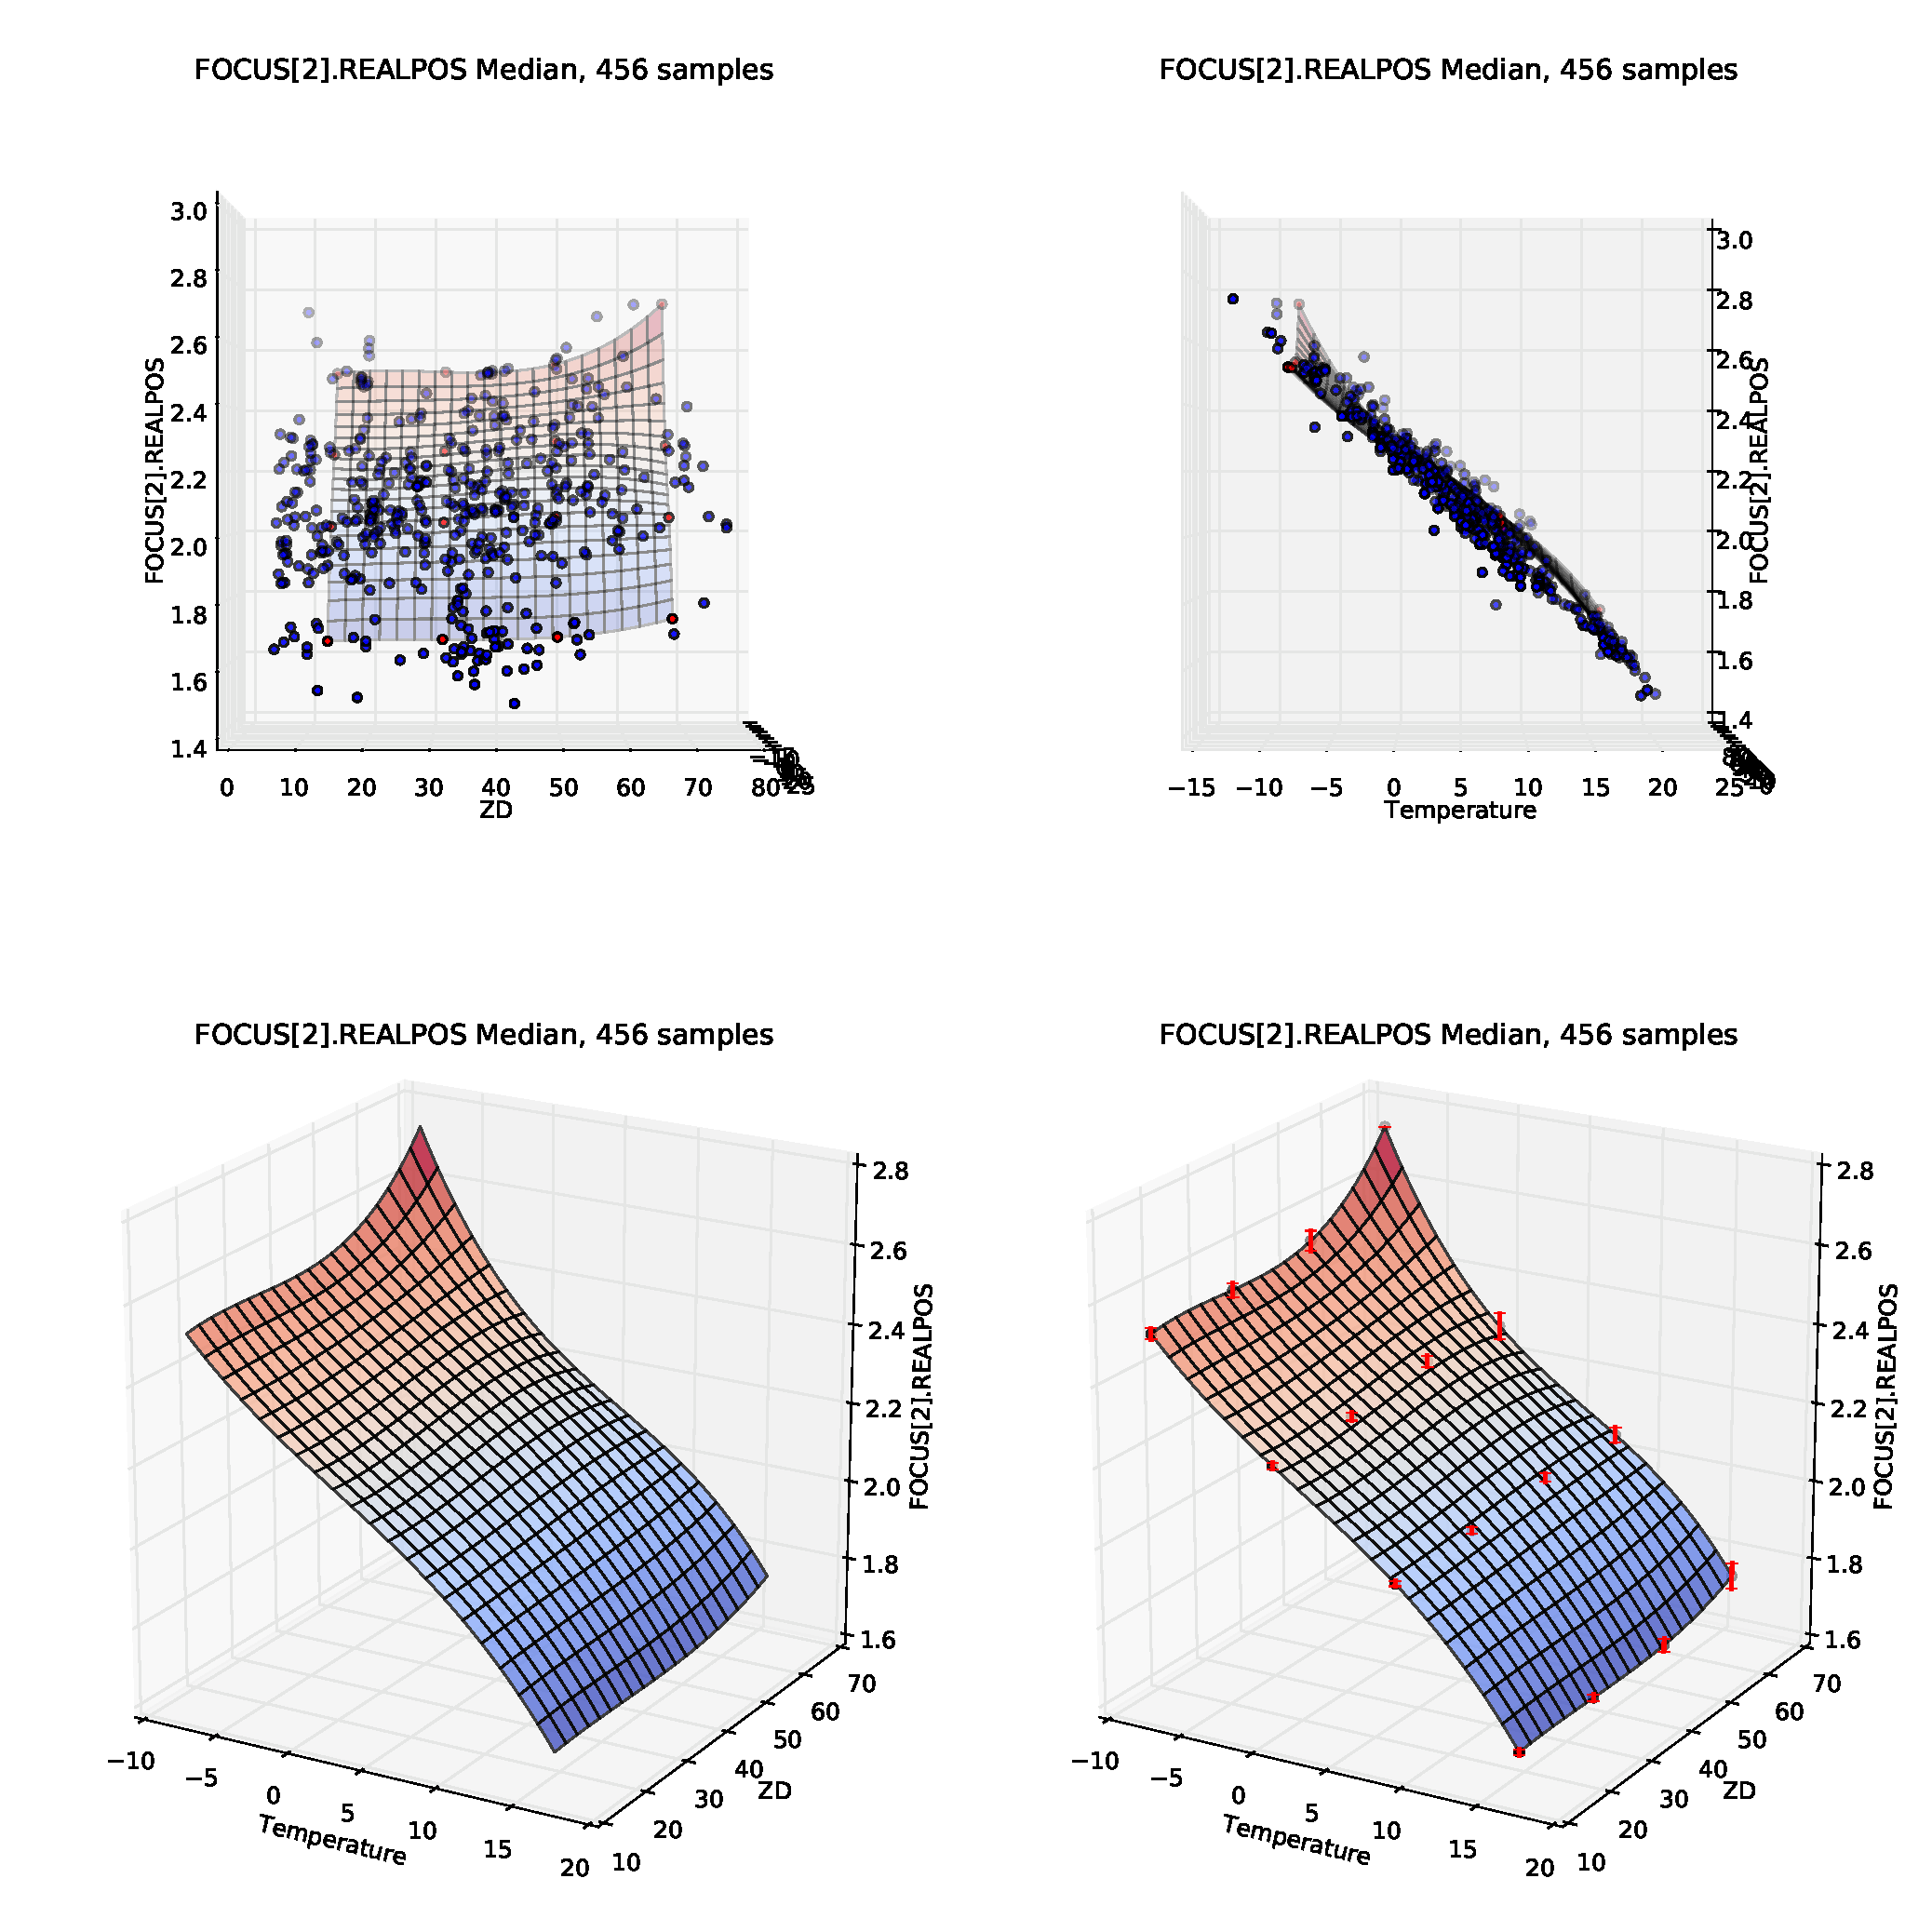
\includegraphics[scale=.44]{tsi_surf/POSITION_INSTRUMENTAL_FOCUS_2__REALPOS_med.pdf}
	\caption[Median Streu- und Flächenplot des Sekundärspiegels]{Median Streu- und Flächenplot des Sekundärspiegels}
    \label{foc_med}
\end{figure}
\begin{figure}[H]
	\centering
	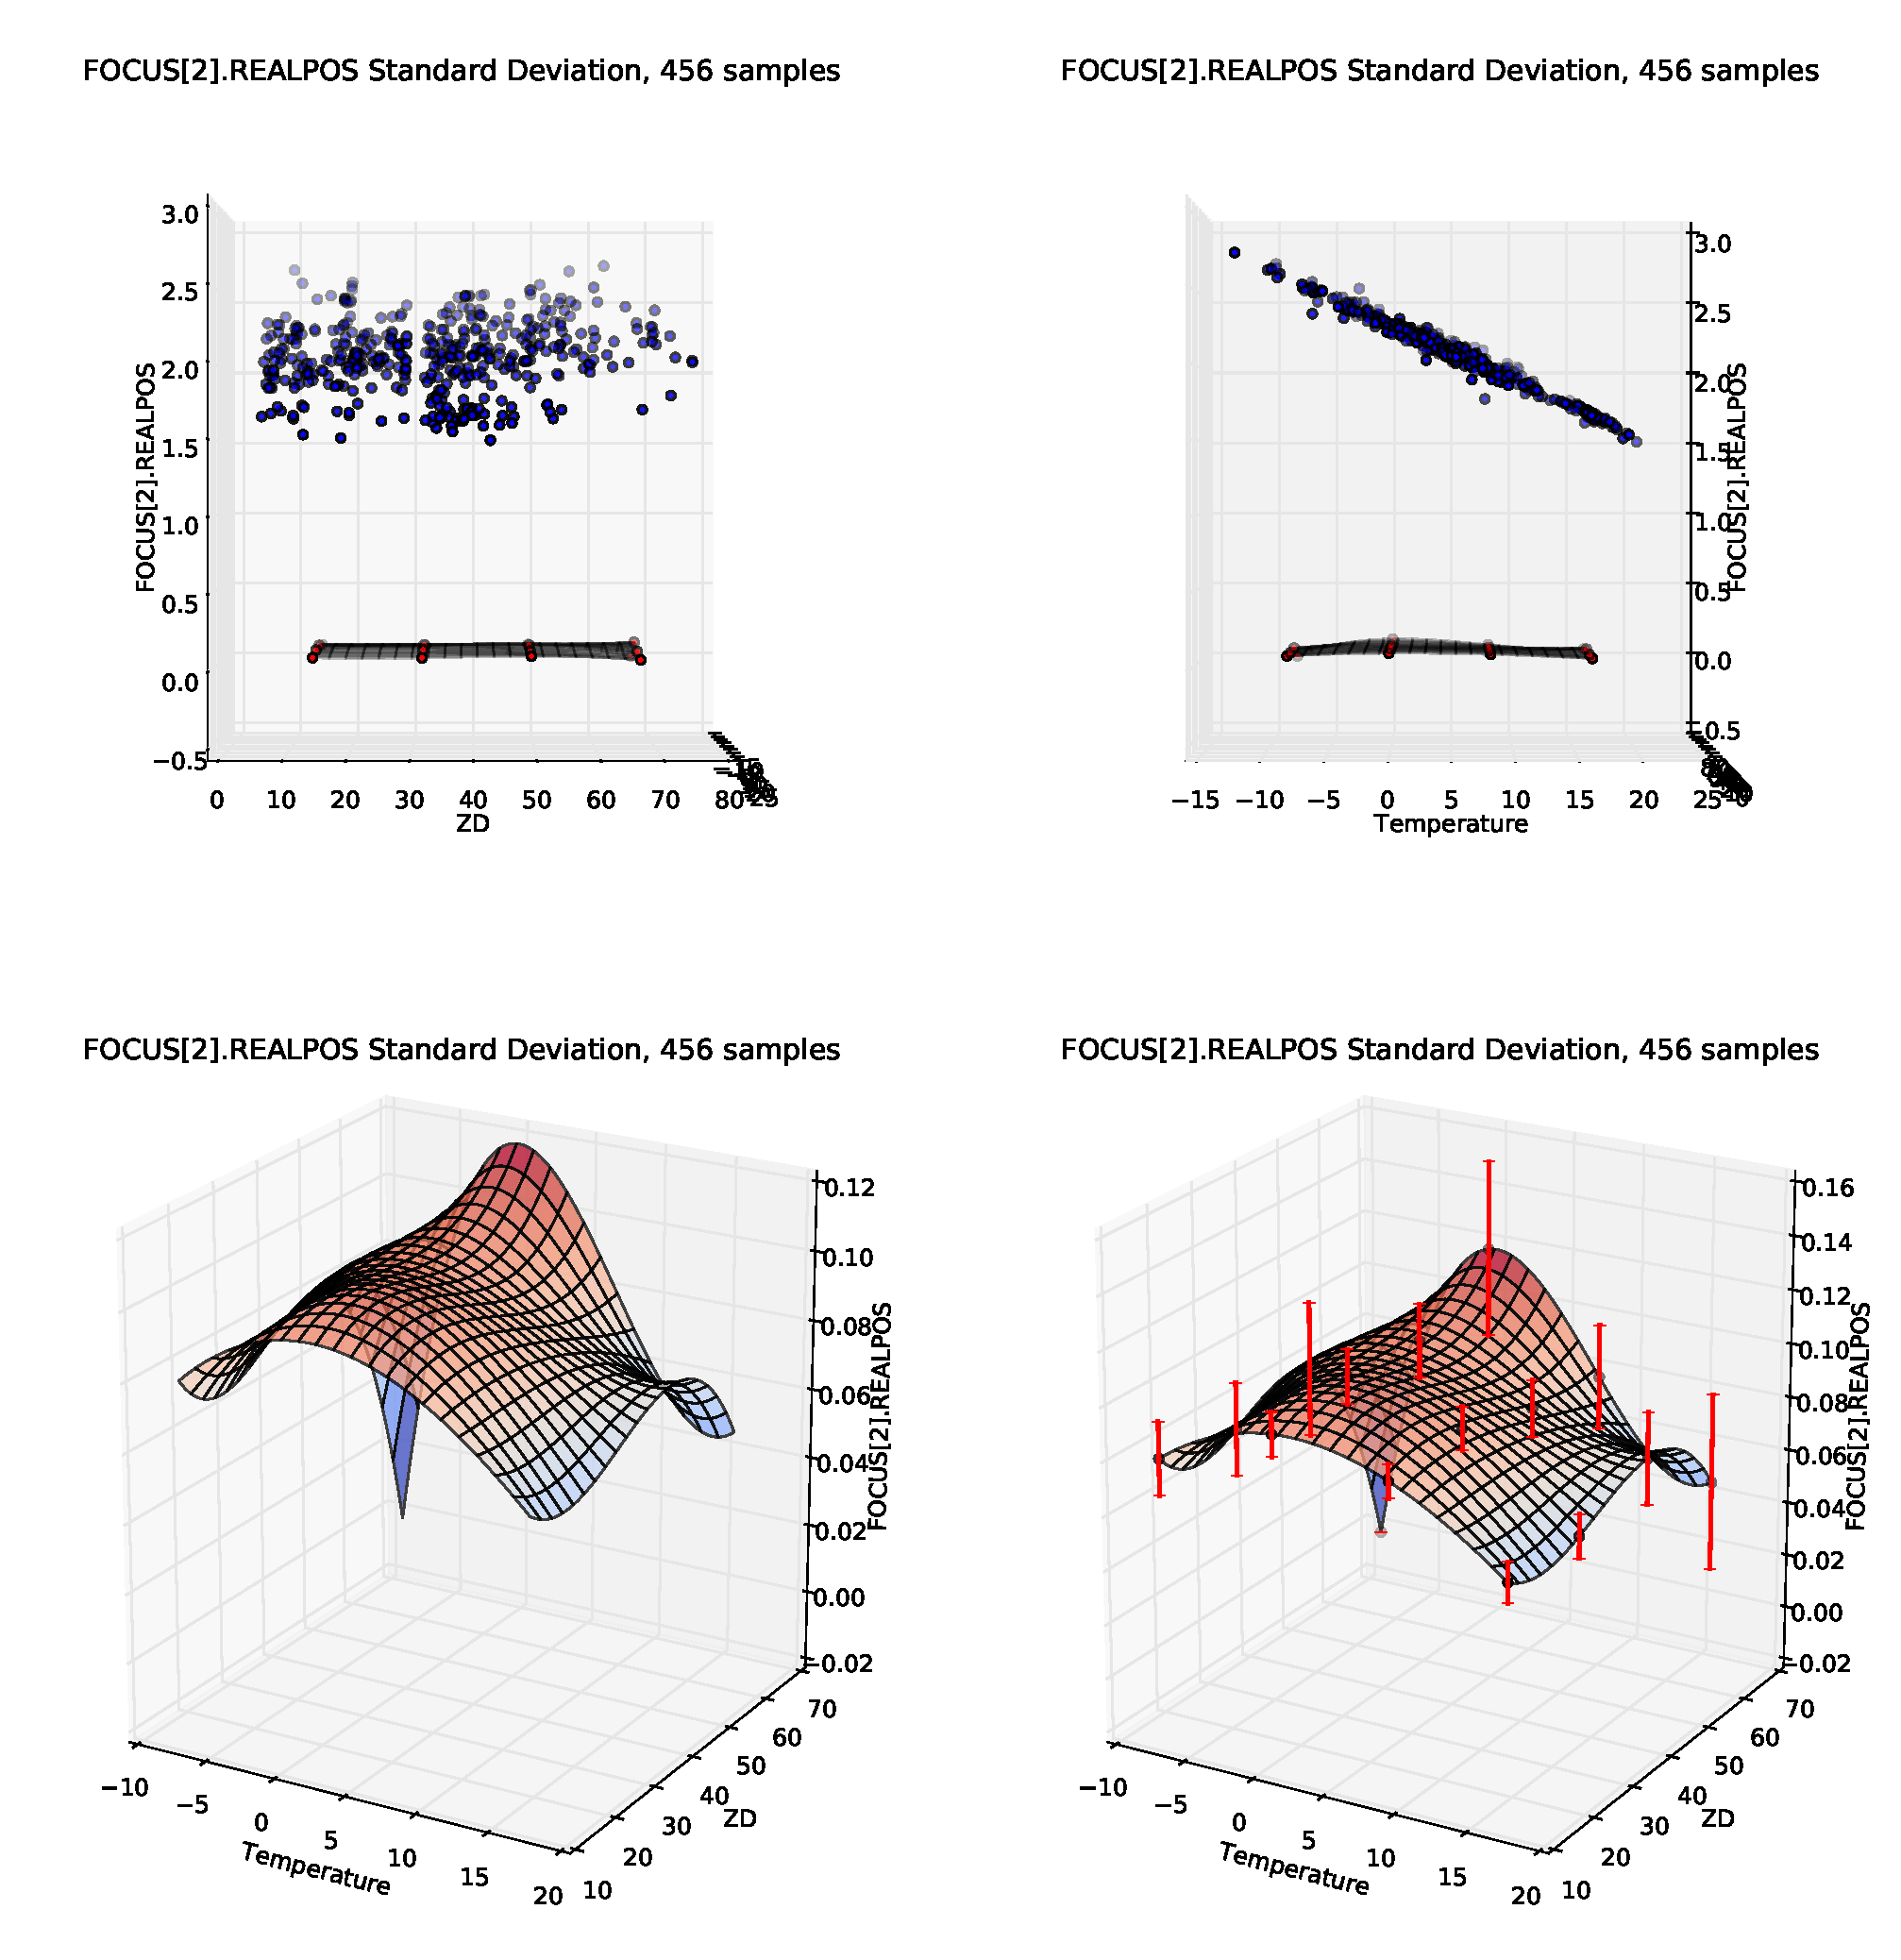
\includegraphics[scale=.44]{tsi_surf/POSITION_INSTRUMENTAL_FOCUS_2__REALPOS_std.pdf}
	\caption[Standardabweichung Streu- und Flächenplot des Sekundärspiegels]{Standardabweichung Streu- und Flächenplot des Sekundärspiegels}
    \label{foc_std}
\end{figure}
\begin{figure}[H]
	\centering
	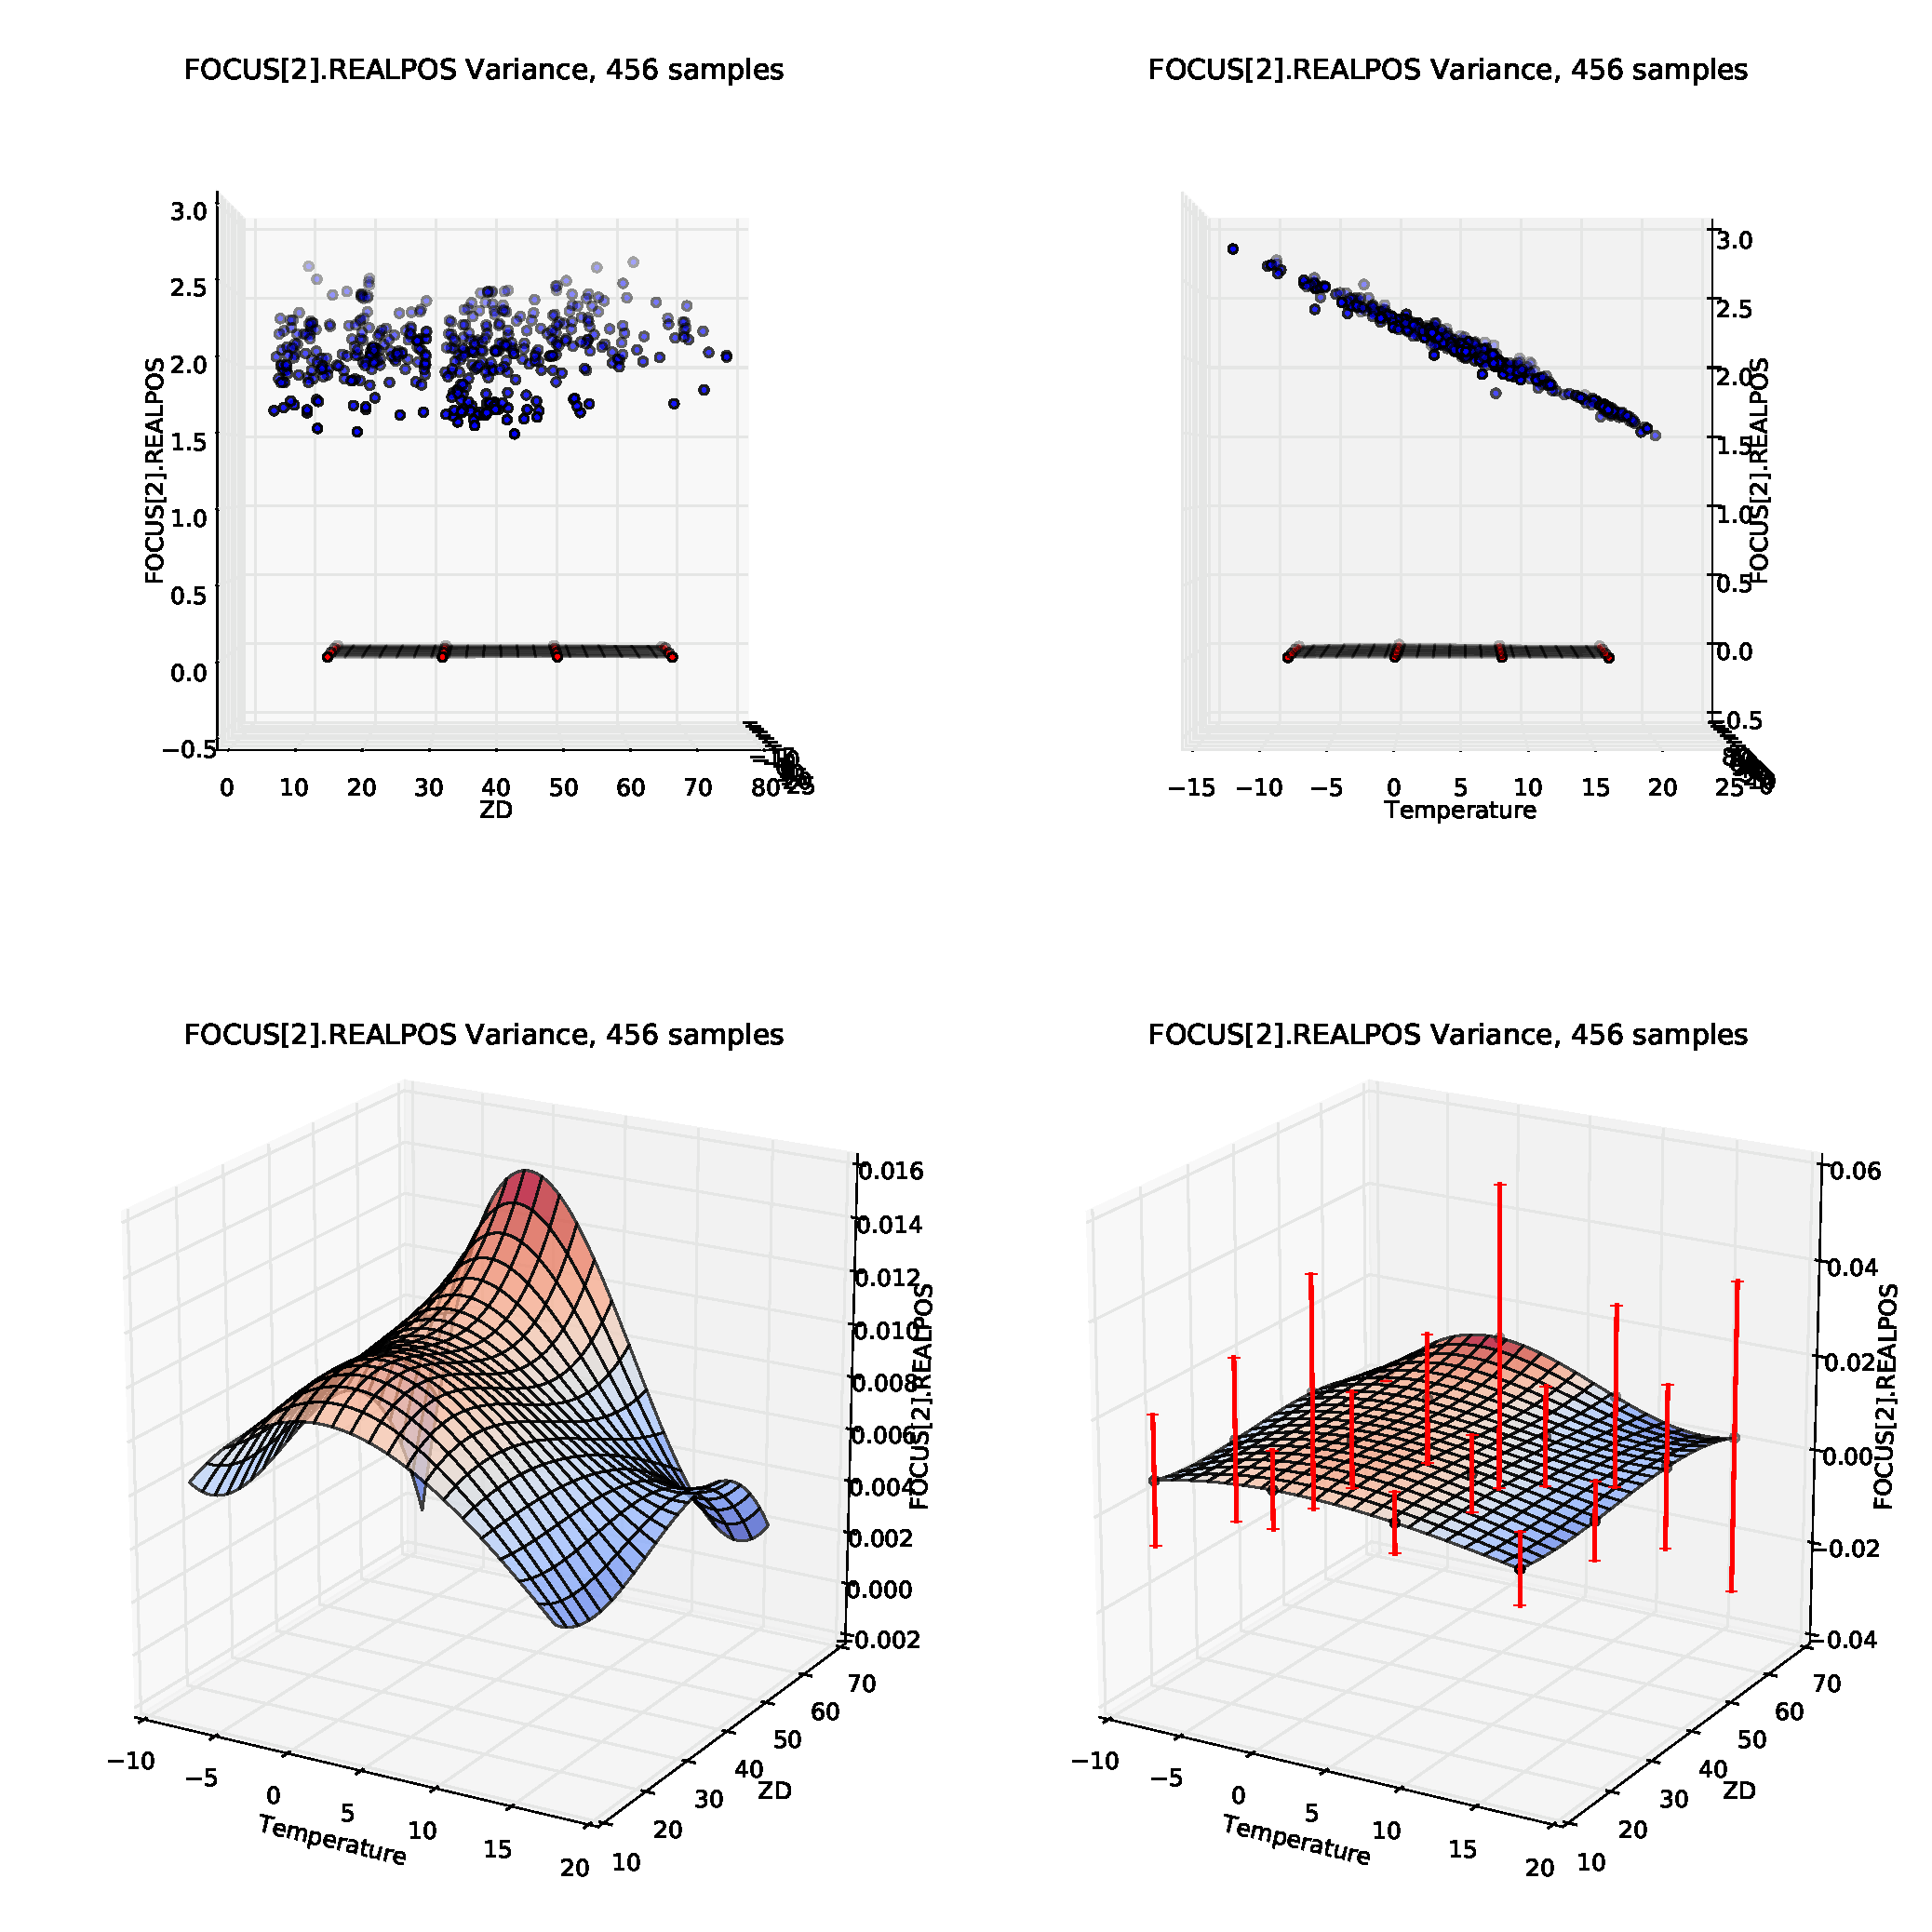
\includegraphics[scale=.44]{tsi_surf/POSITION_INSTRUMENTAL_FOCUS_2__REALPOS_var.pdf}
	\caption[Varianz Streu- und Flächenplot des Sekundärspiegels]{Varianz Streu- und Flächenplot des Sekundärspiegels}
    \label{foc_var}
\end{figure}

\section{Transinformation Korrelationsmatrizen}

\begin{figure}[H]
	\centering
	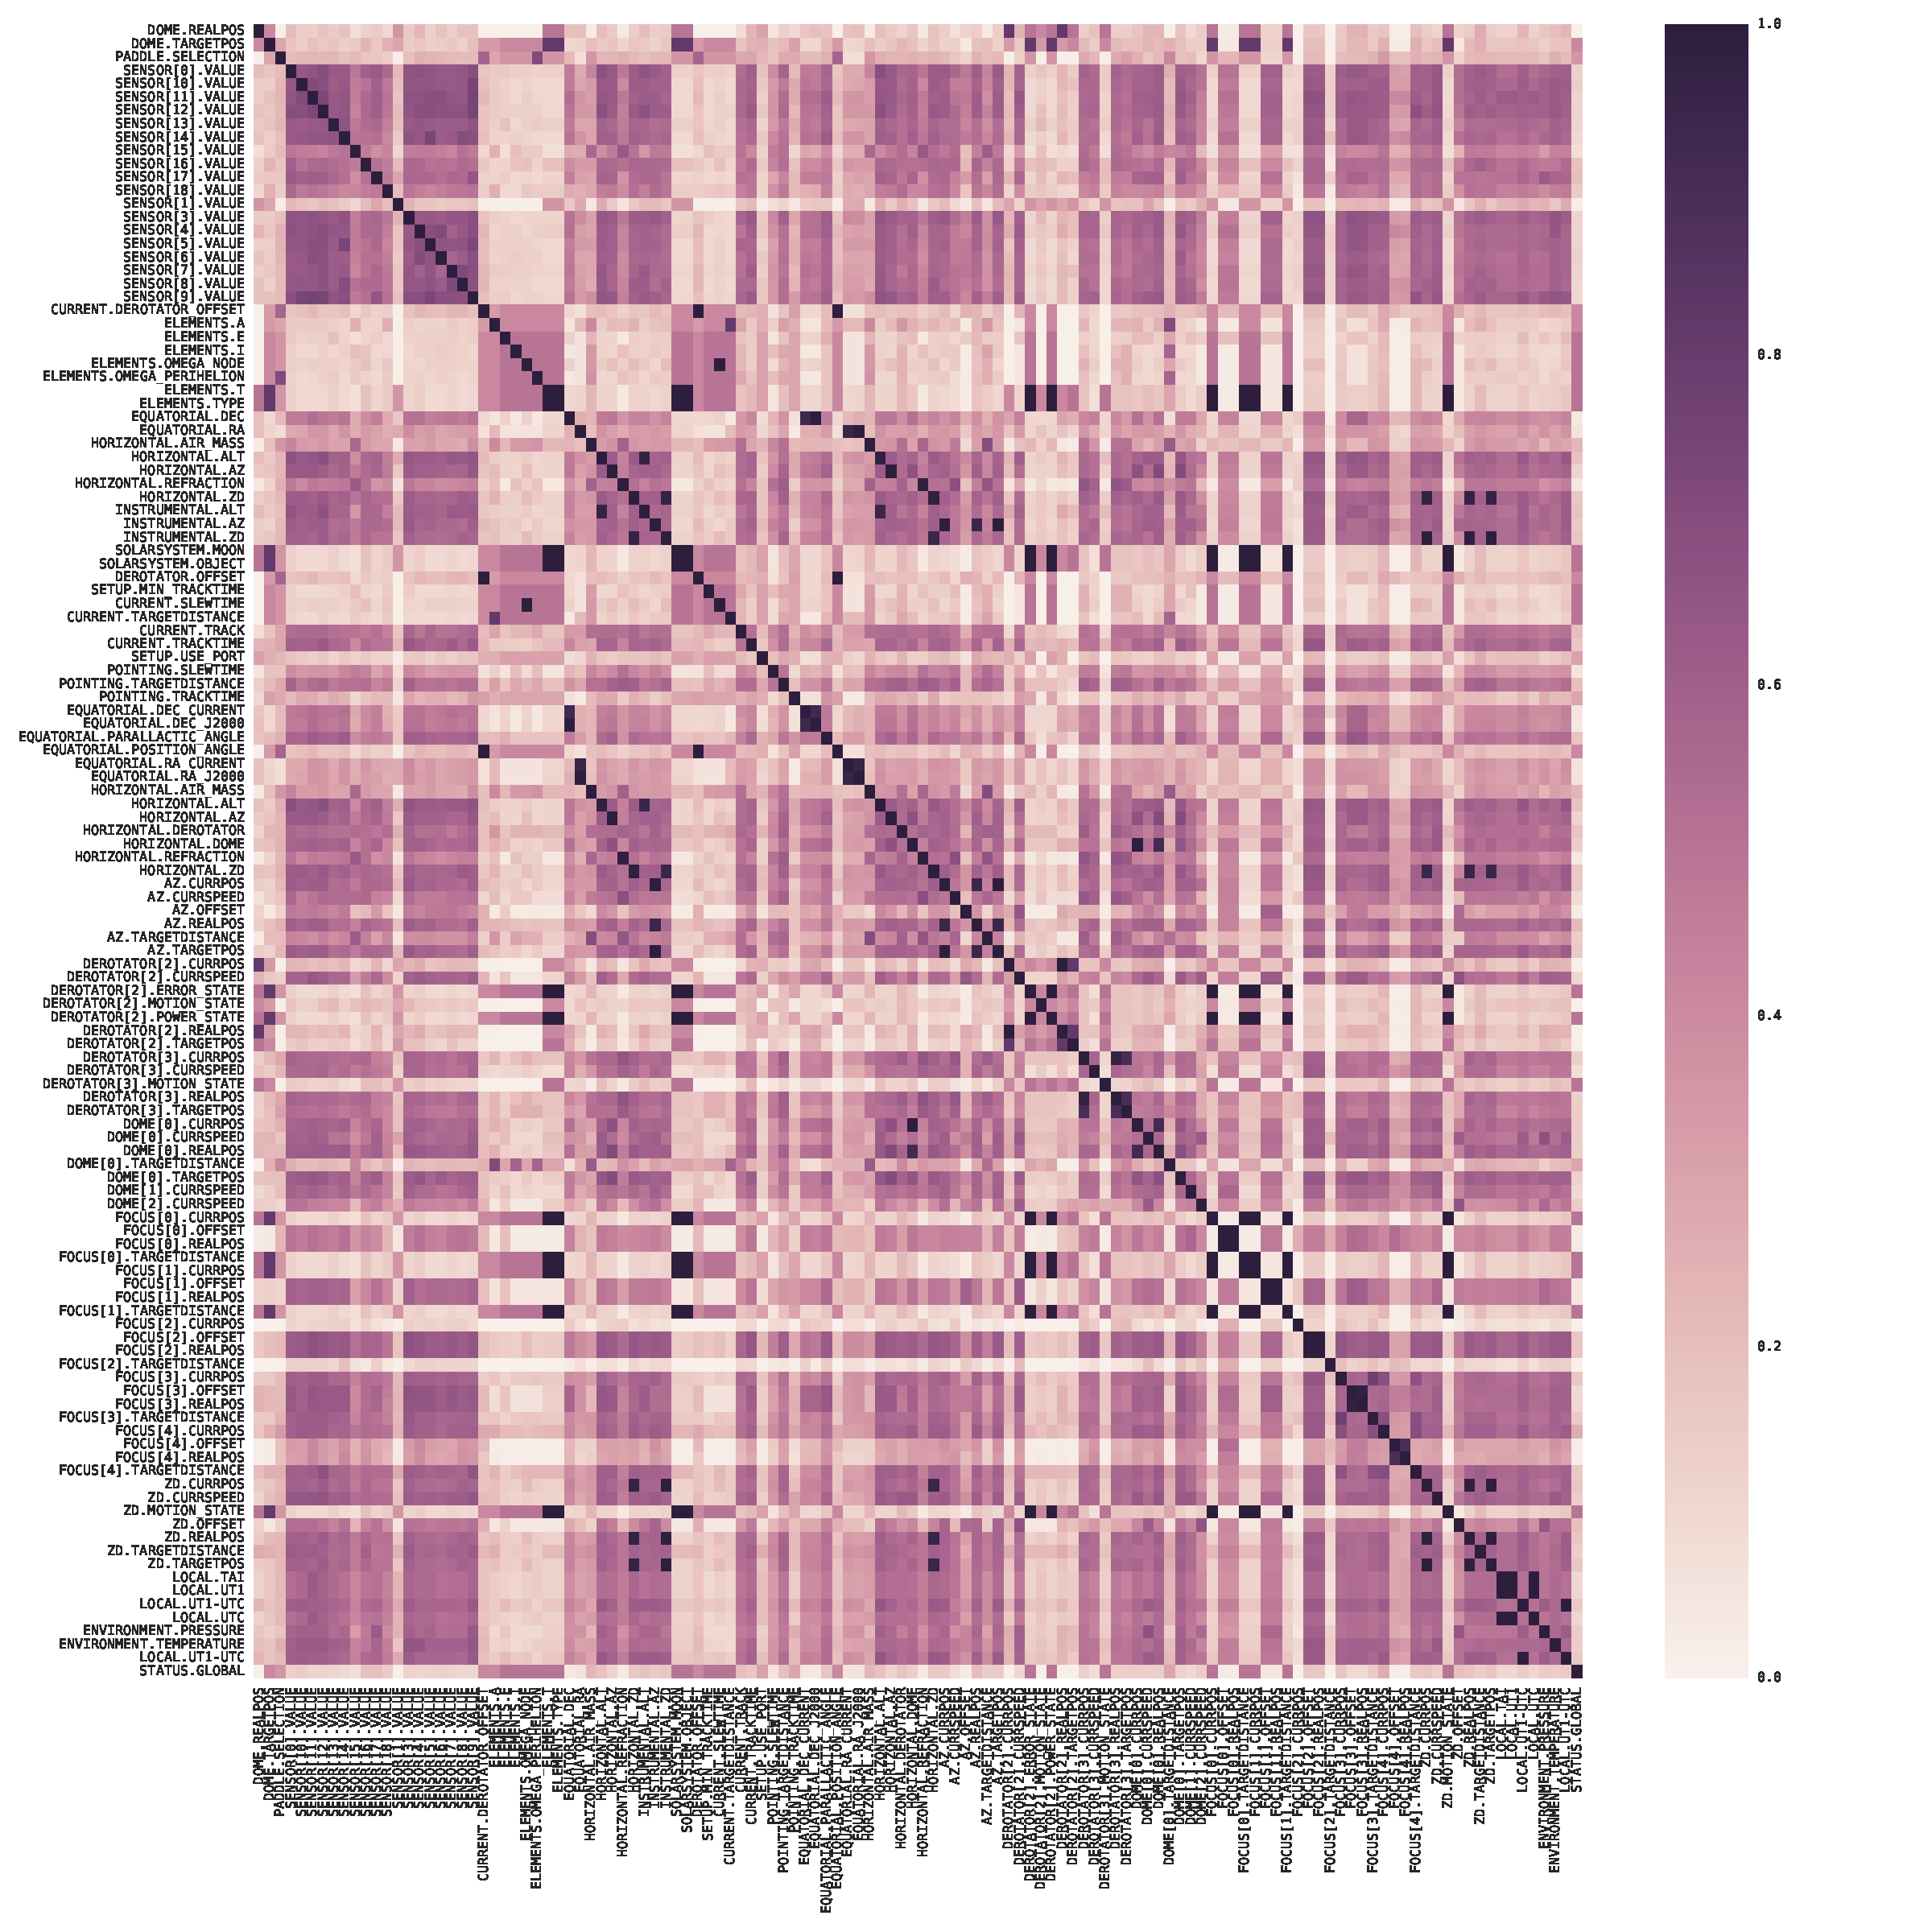
\includegraphics[scale=.44]{heatmaps/tsi.pdf}
	\caption[Heatmap der Transinformation Korrelationsmatrix der TSI-Parameter]{Heatmap der Transinformation Korrelationsmatrix der TSI-Parameter}
    \label{heatmap_tsi}
\end{figure}
\begin{figure}[H]
	\centering
	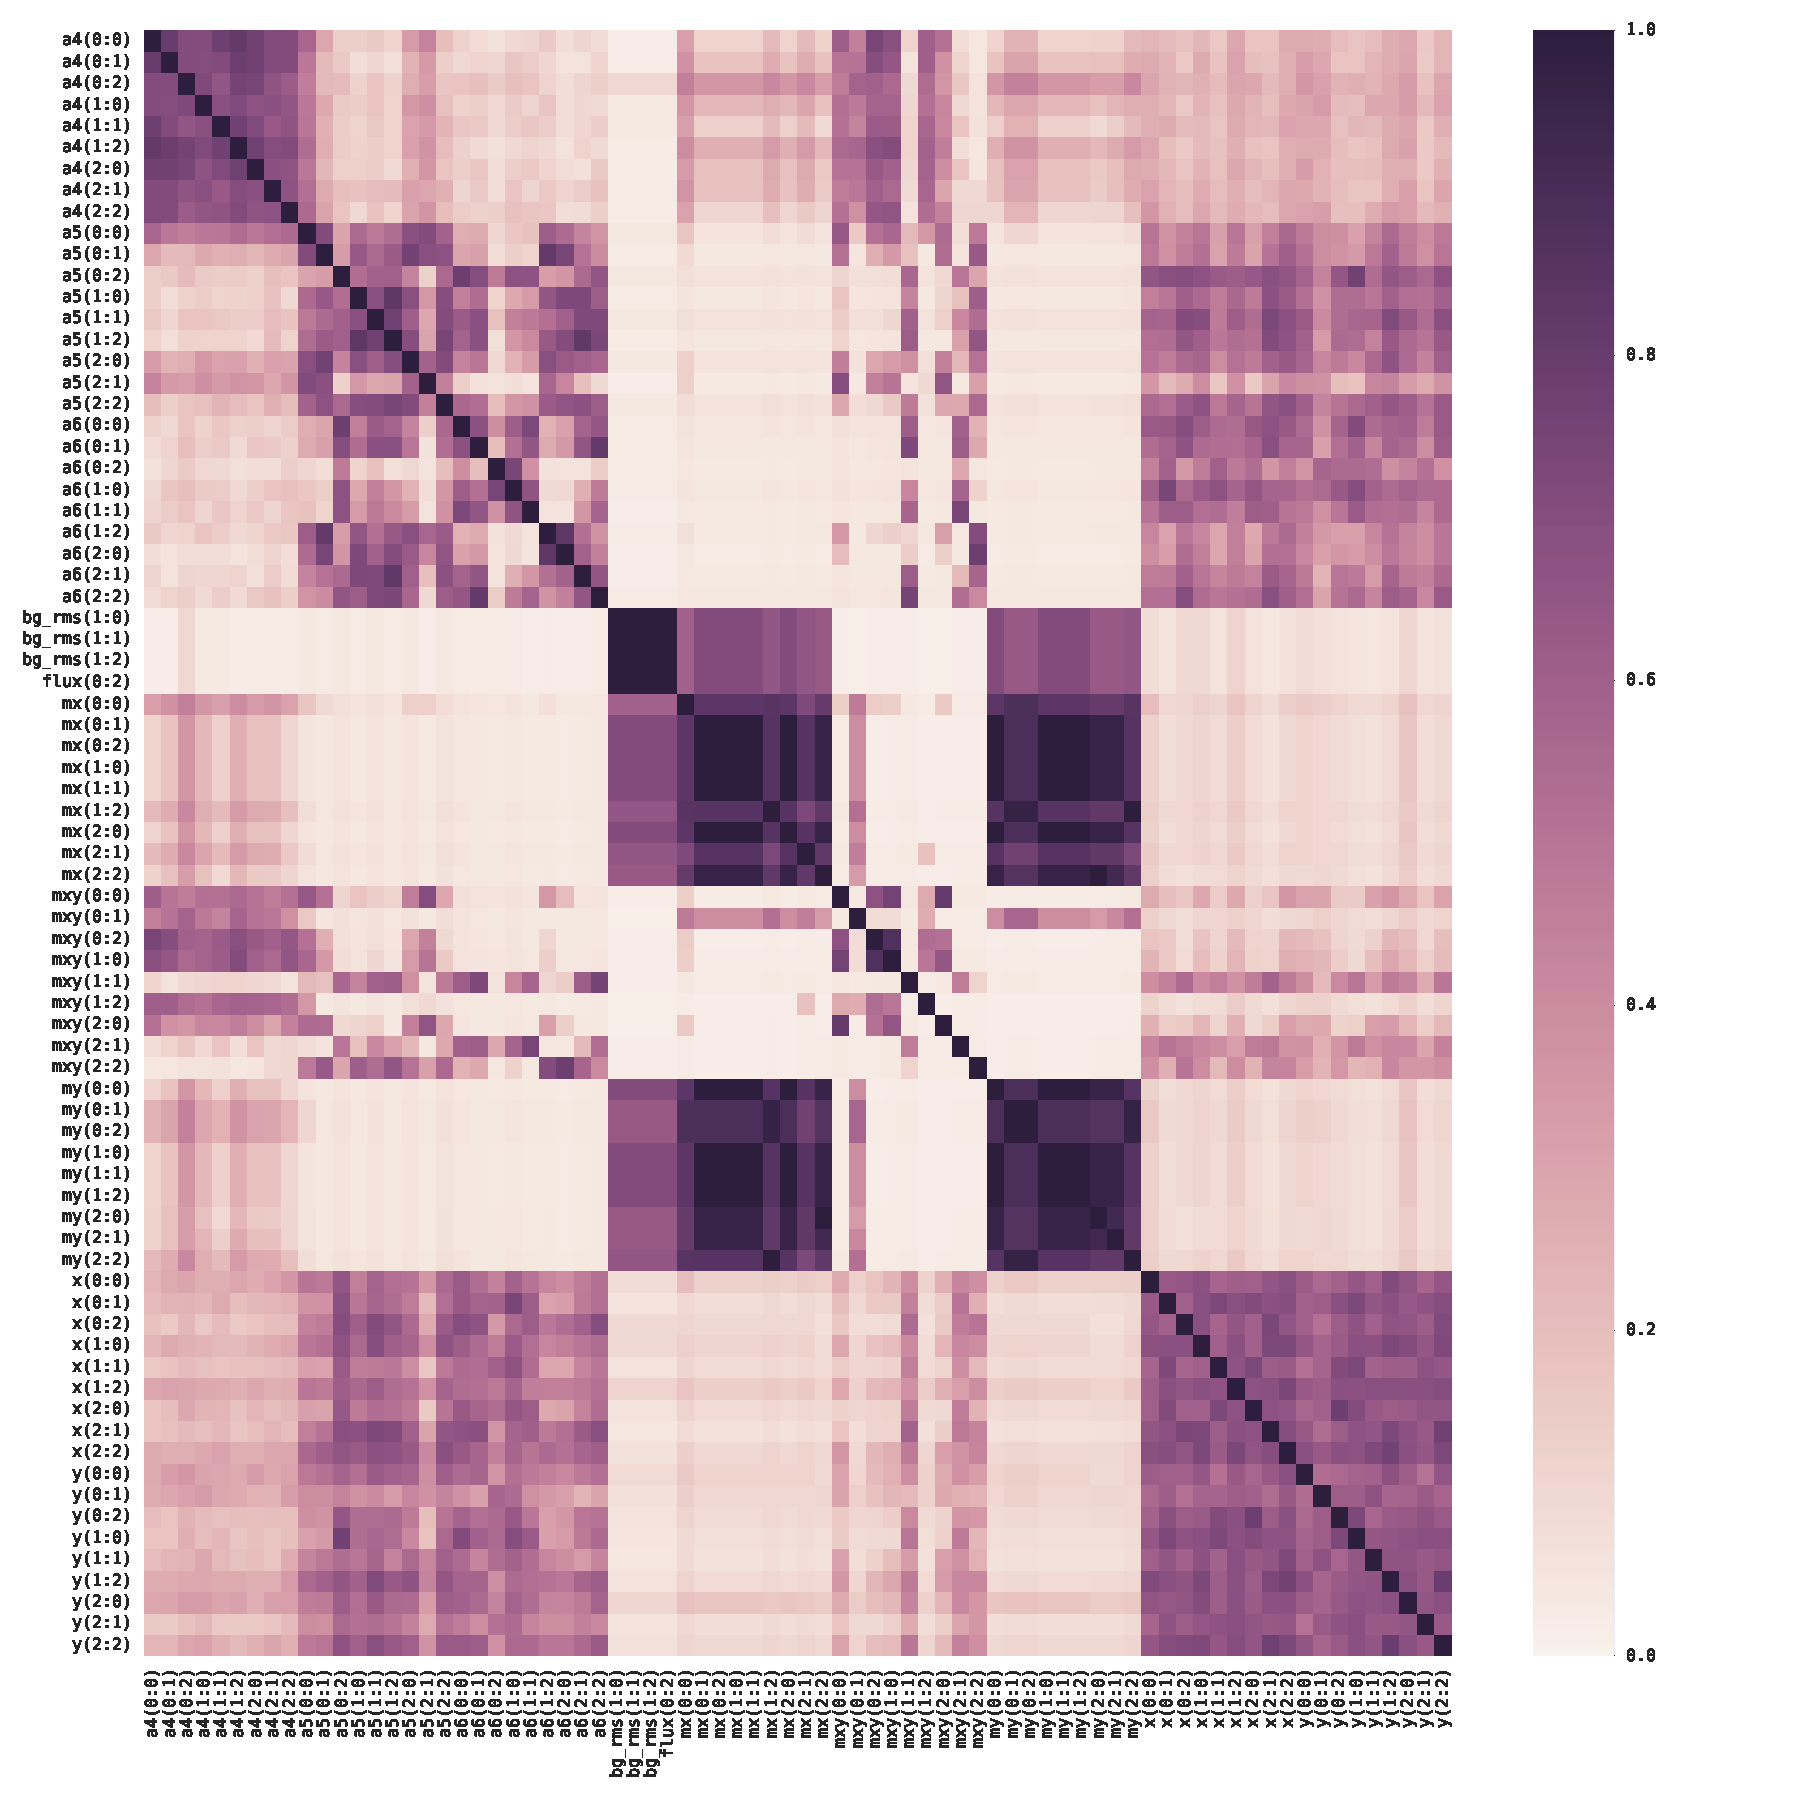
\includegraphics[scale=.58]{heatmaps/psf.pdf}
	\caption[Heatmap der Transinformation Korrelationsmatrix der PSF-Parameter]{Heatmap der Transinformation Korrelationsmatrix der PSF-Parameter}
    \label{heatmap_psf}
\end{figure}
\begin{figure}[H]
	\centering
	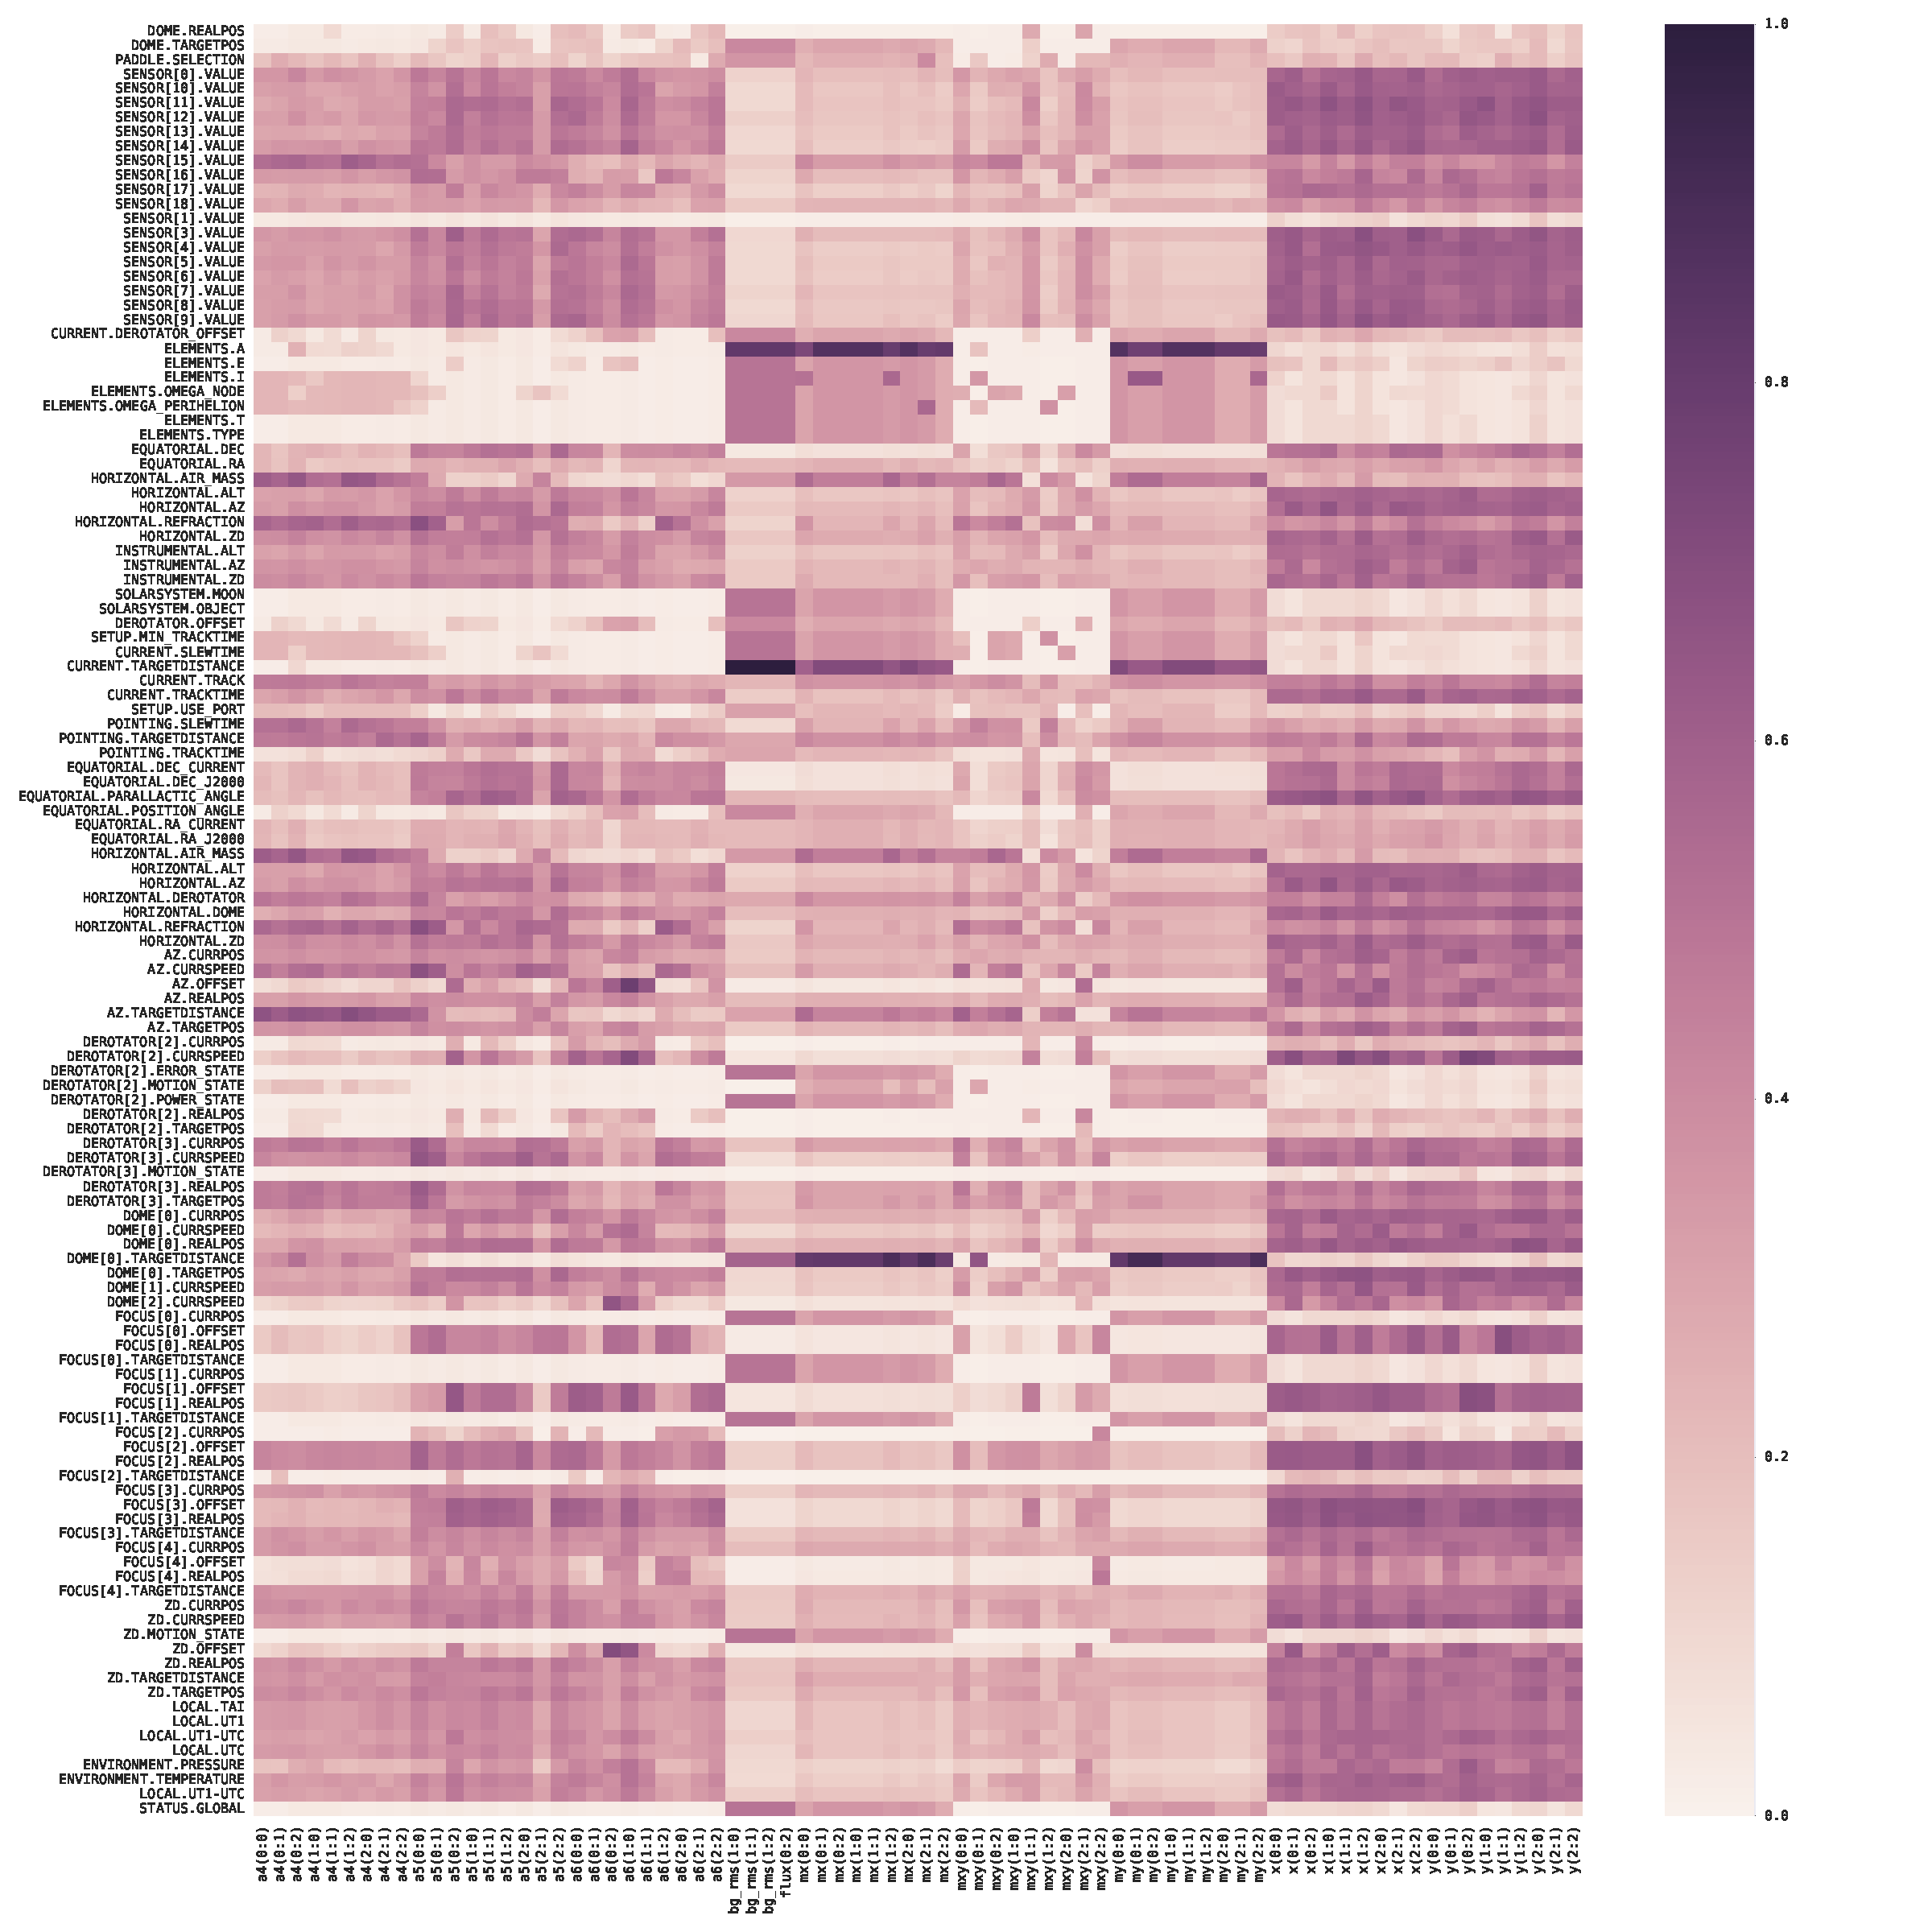
\includegraphics[scale=.44]{heatmaps/psf_tsi.pdf}
	\caption[Heatmap der Transinformation Korrelationsmatrix zwischen PSF- und TSI-Parametern]{Heatmap der Transinformation Korrelationsmatrix zwischen PSF- und TSI-Parametern}
    \label{heatmap_psf_tsi}
\end{figure}

\section{Windgeschwindigkeit, Windrichtung und PSF-Parameter}
\begin{figure}[H]
	\centering
	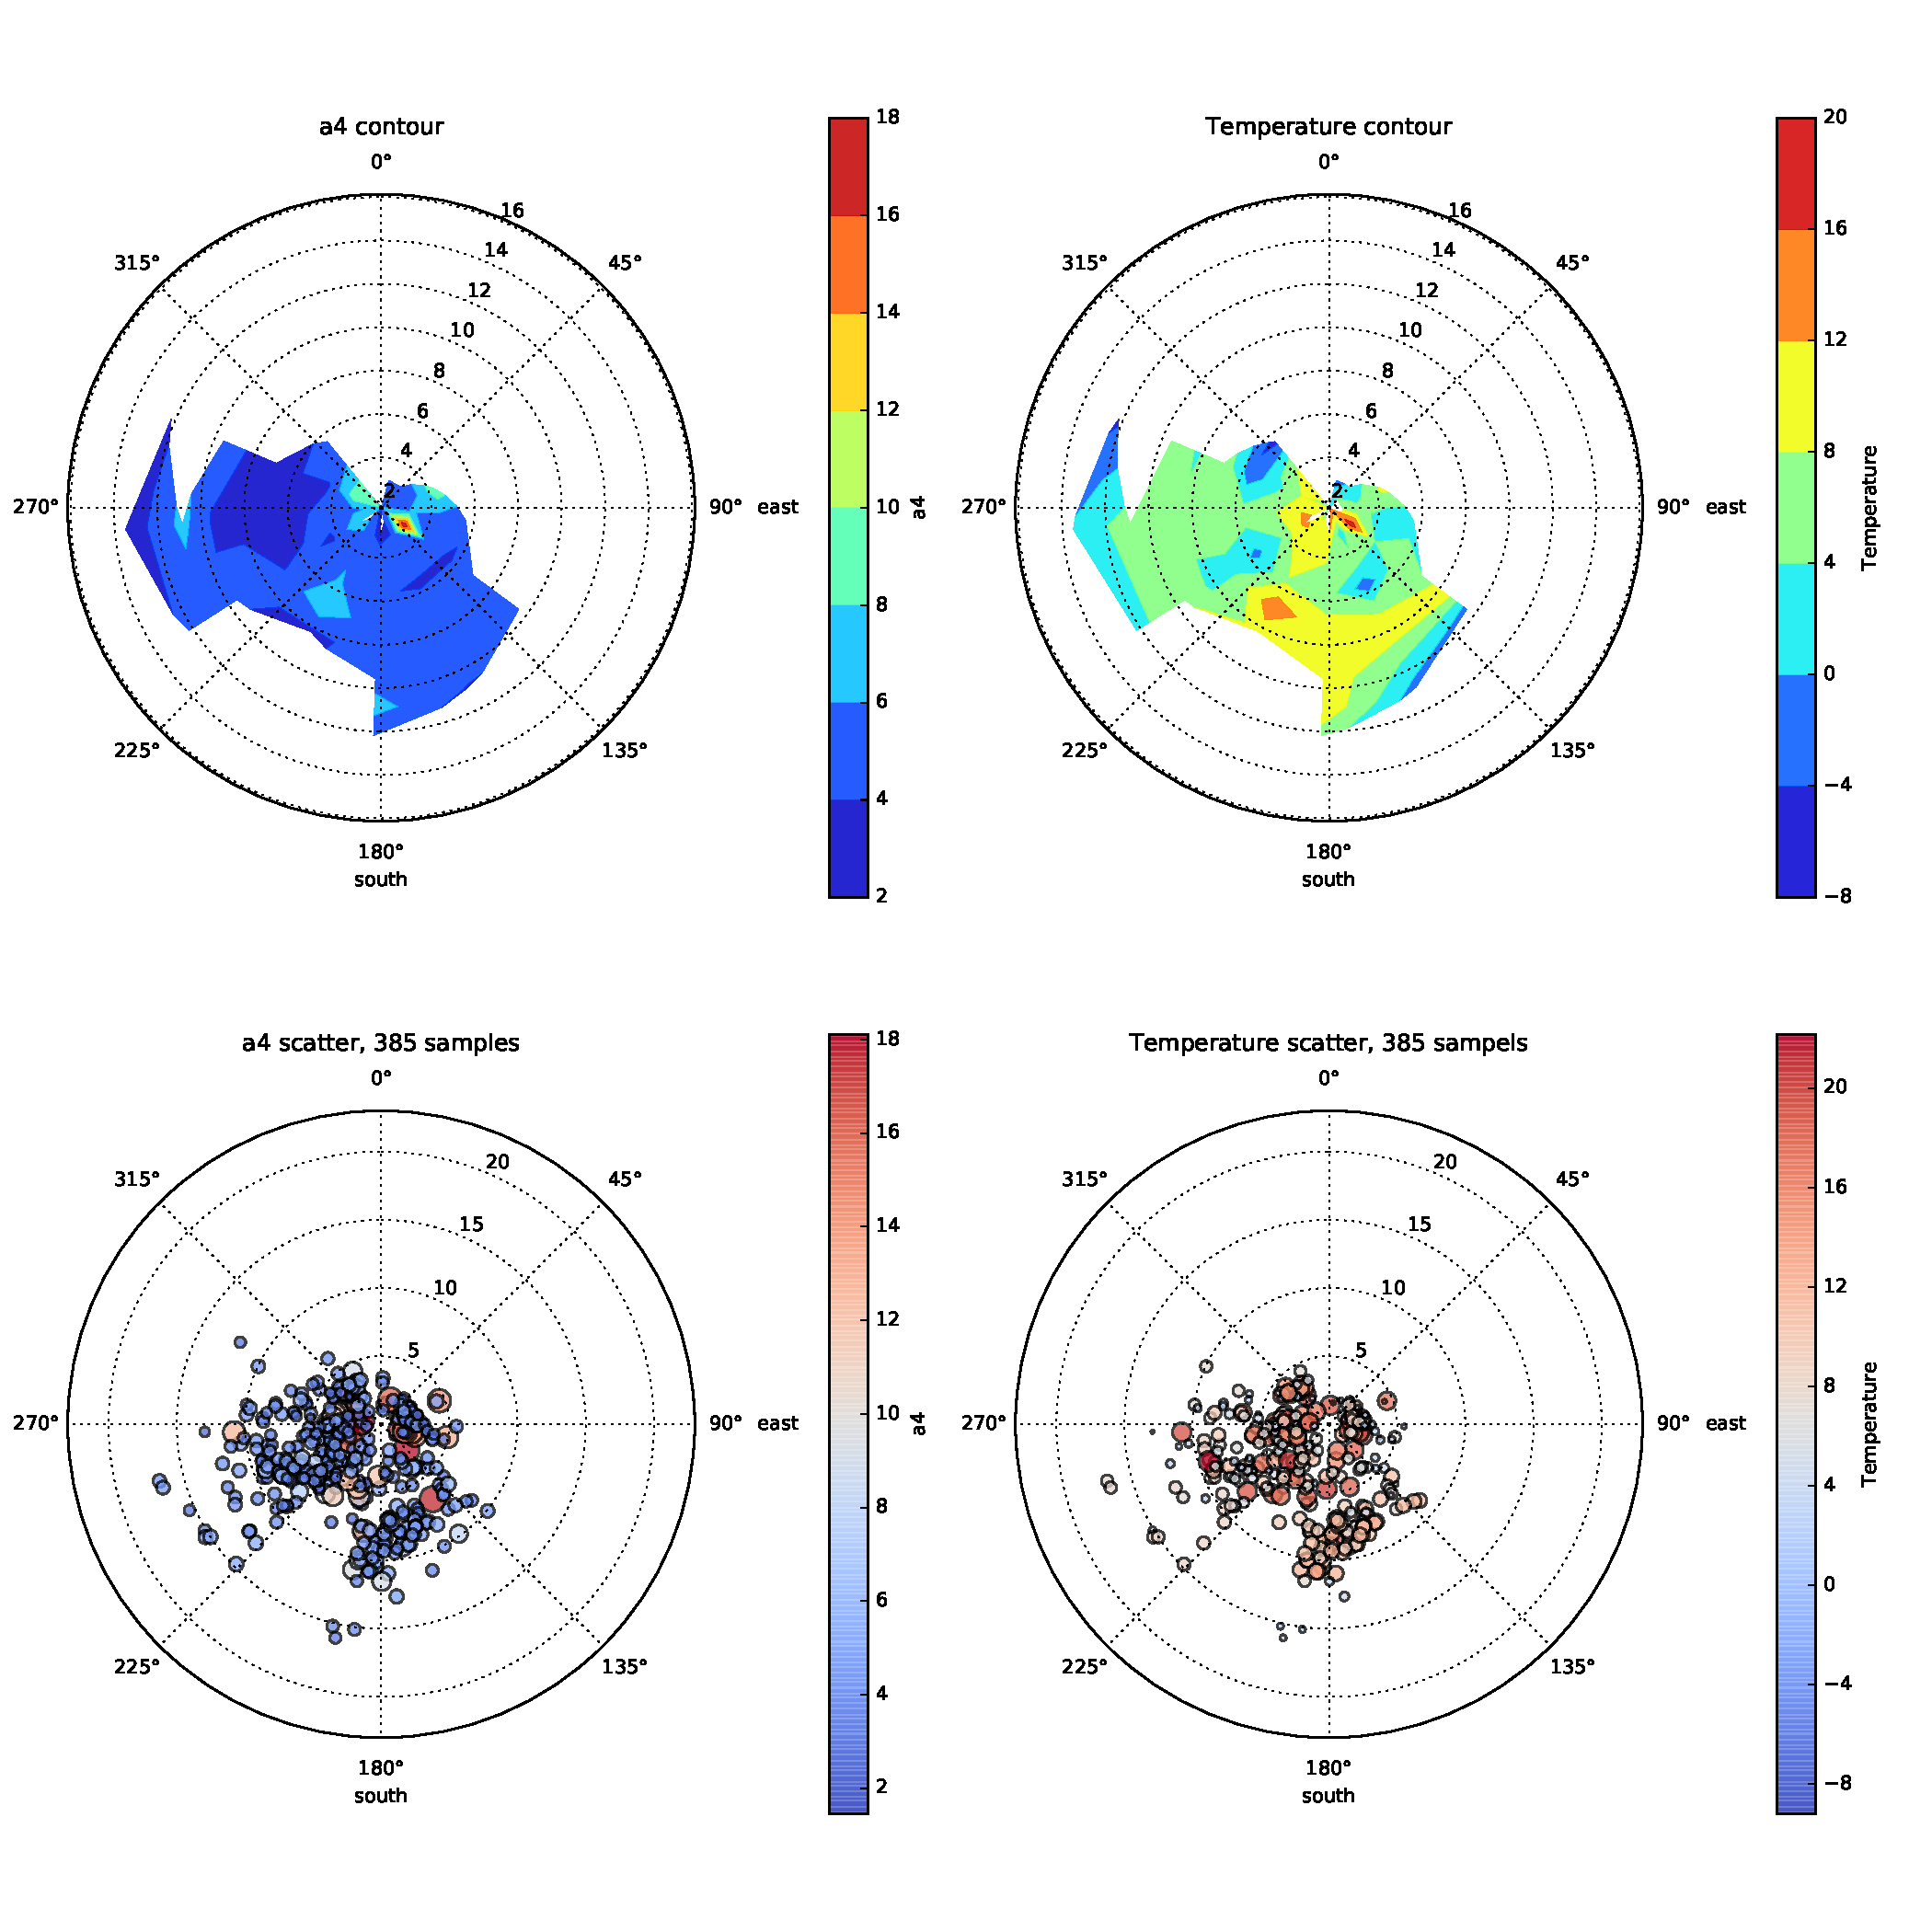
\includegraphics[scale=.46]{wind/wind_a4}
	\caption[Polarplot Windgeschwindigkeit, Windrichtung und $A_4$]{Polarplot Windgeschwindigkeit, Windrichtung und $A_4$}
    \label{wind_a4}
\end{figure}
\begin{figure}[H]
	\centering
	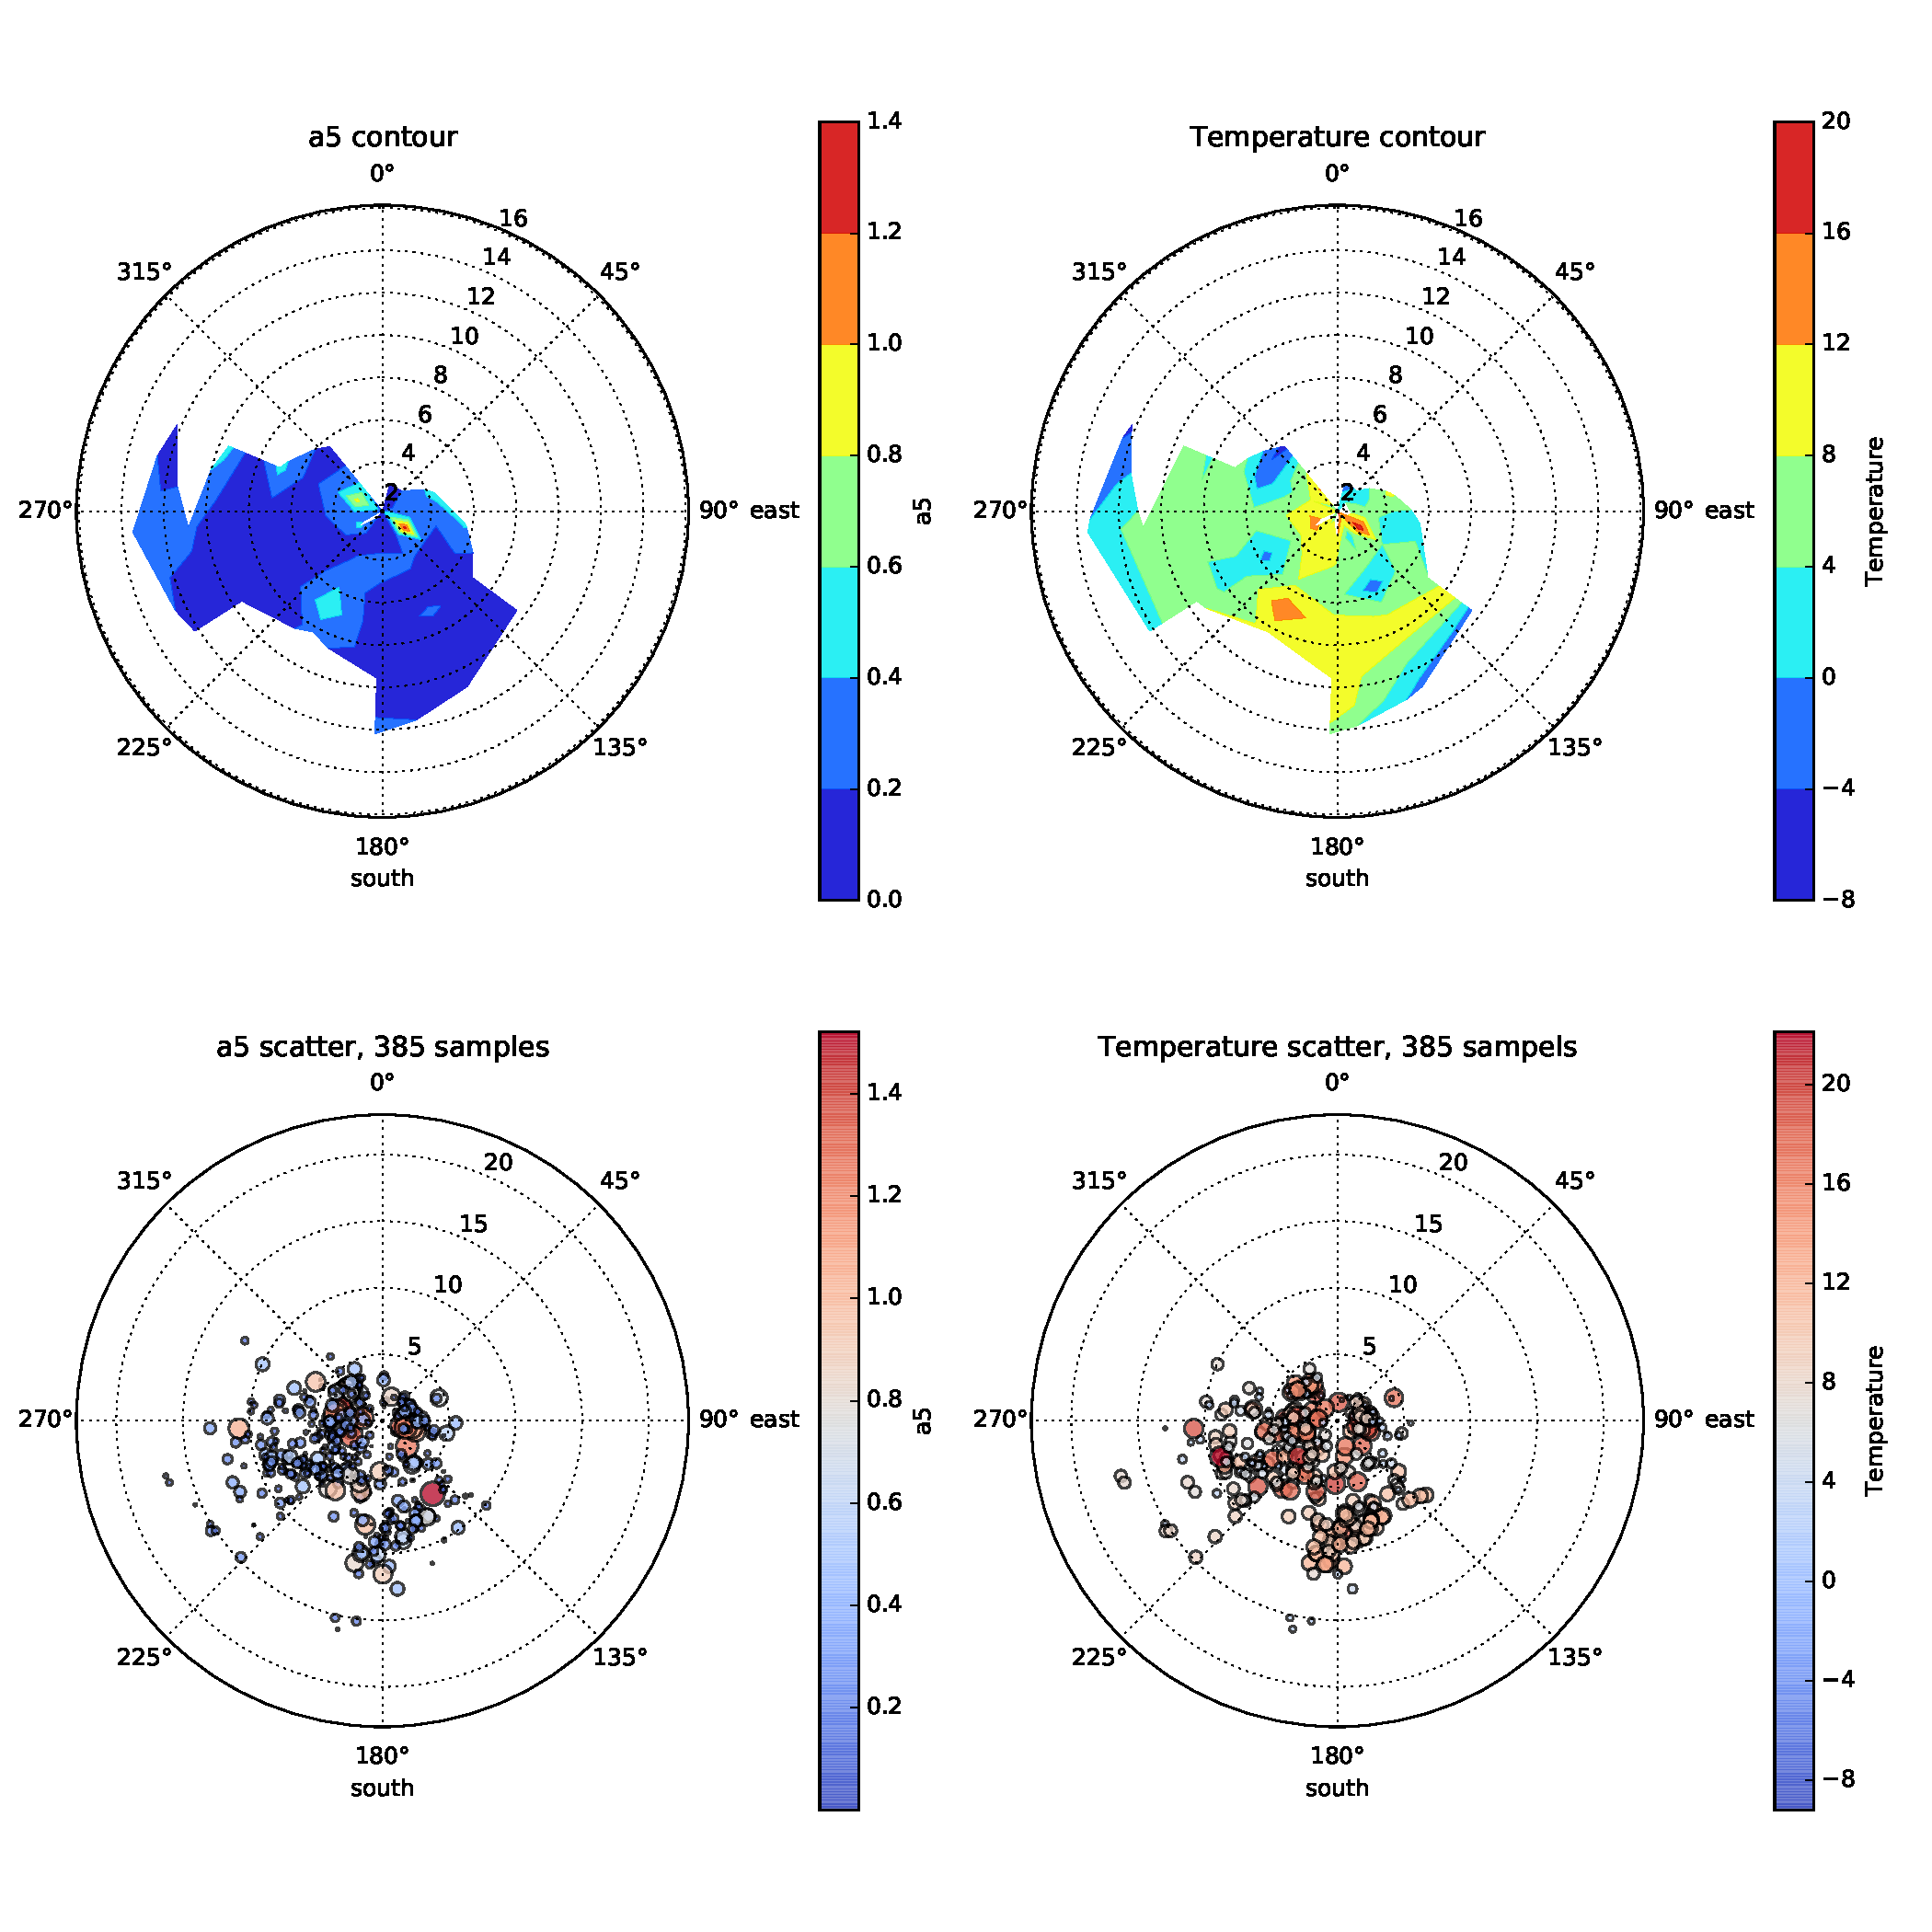
\includegraphics[scale=.46]{wind/wind_a5}
	\caption[Polarplot Windgeschwindigkeit, Windrichtung und $A_5$]{Polarplot Windgeschwindigkeit, Windrichtung und $A_5$}
    \label{wind_a5}
\end{figure}
\begin{figure}[H]
	\centering
	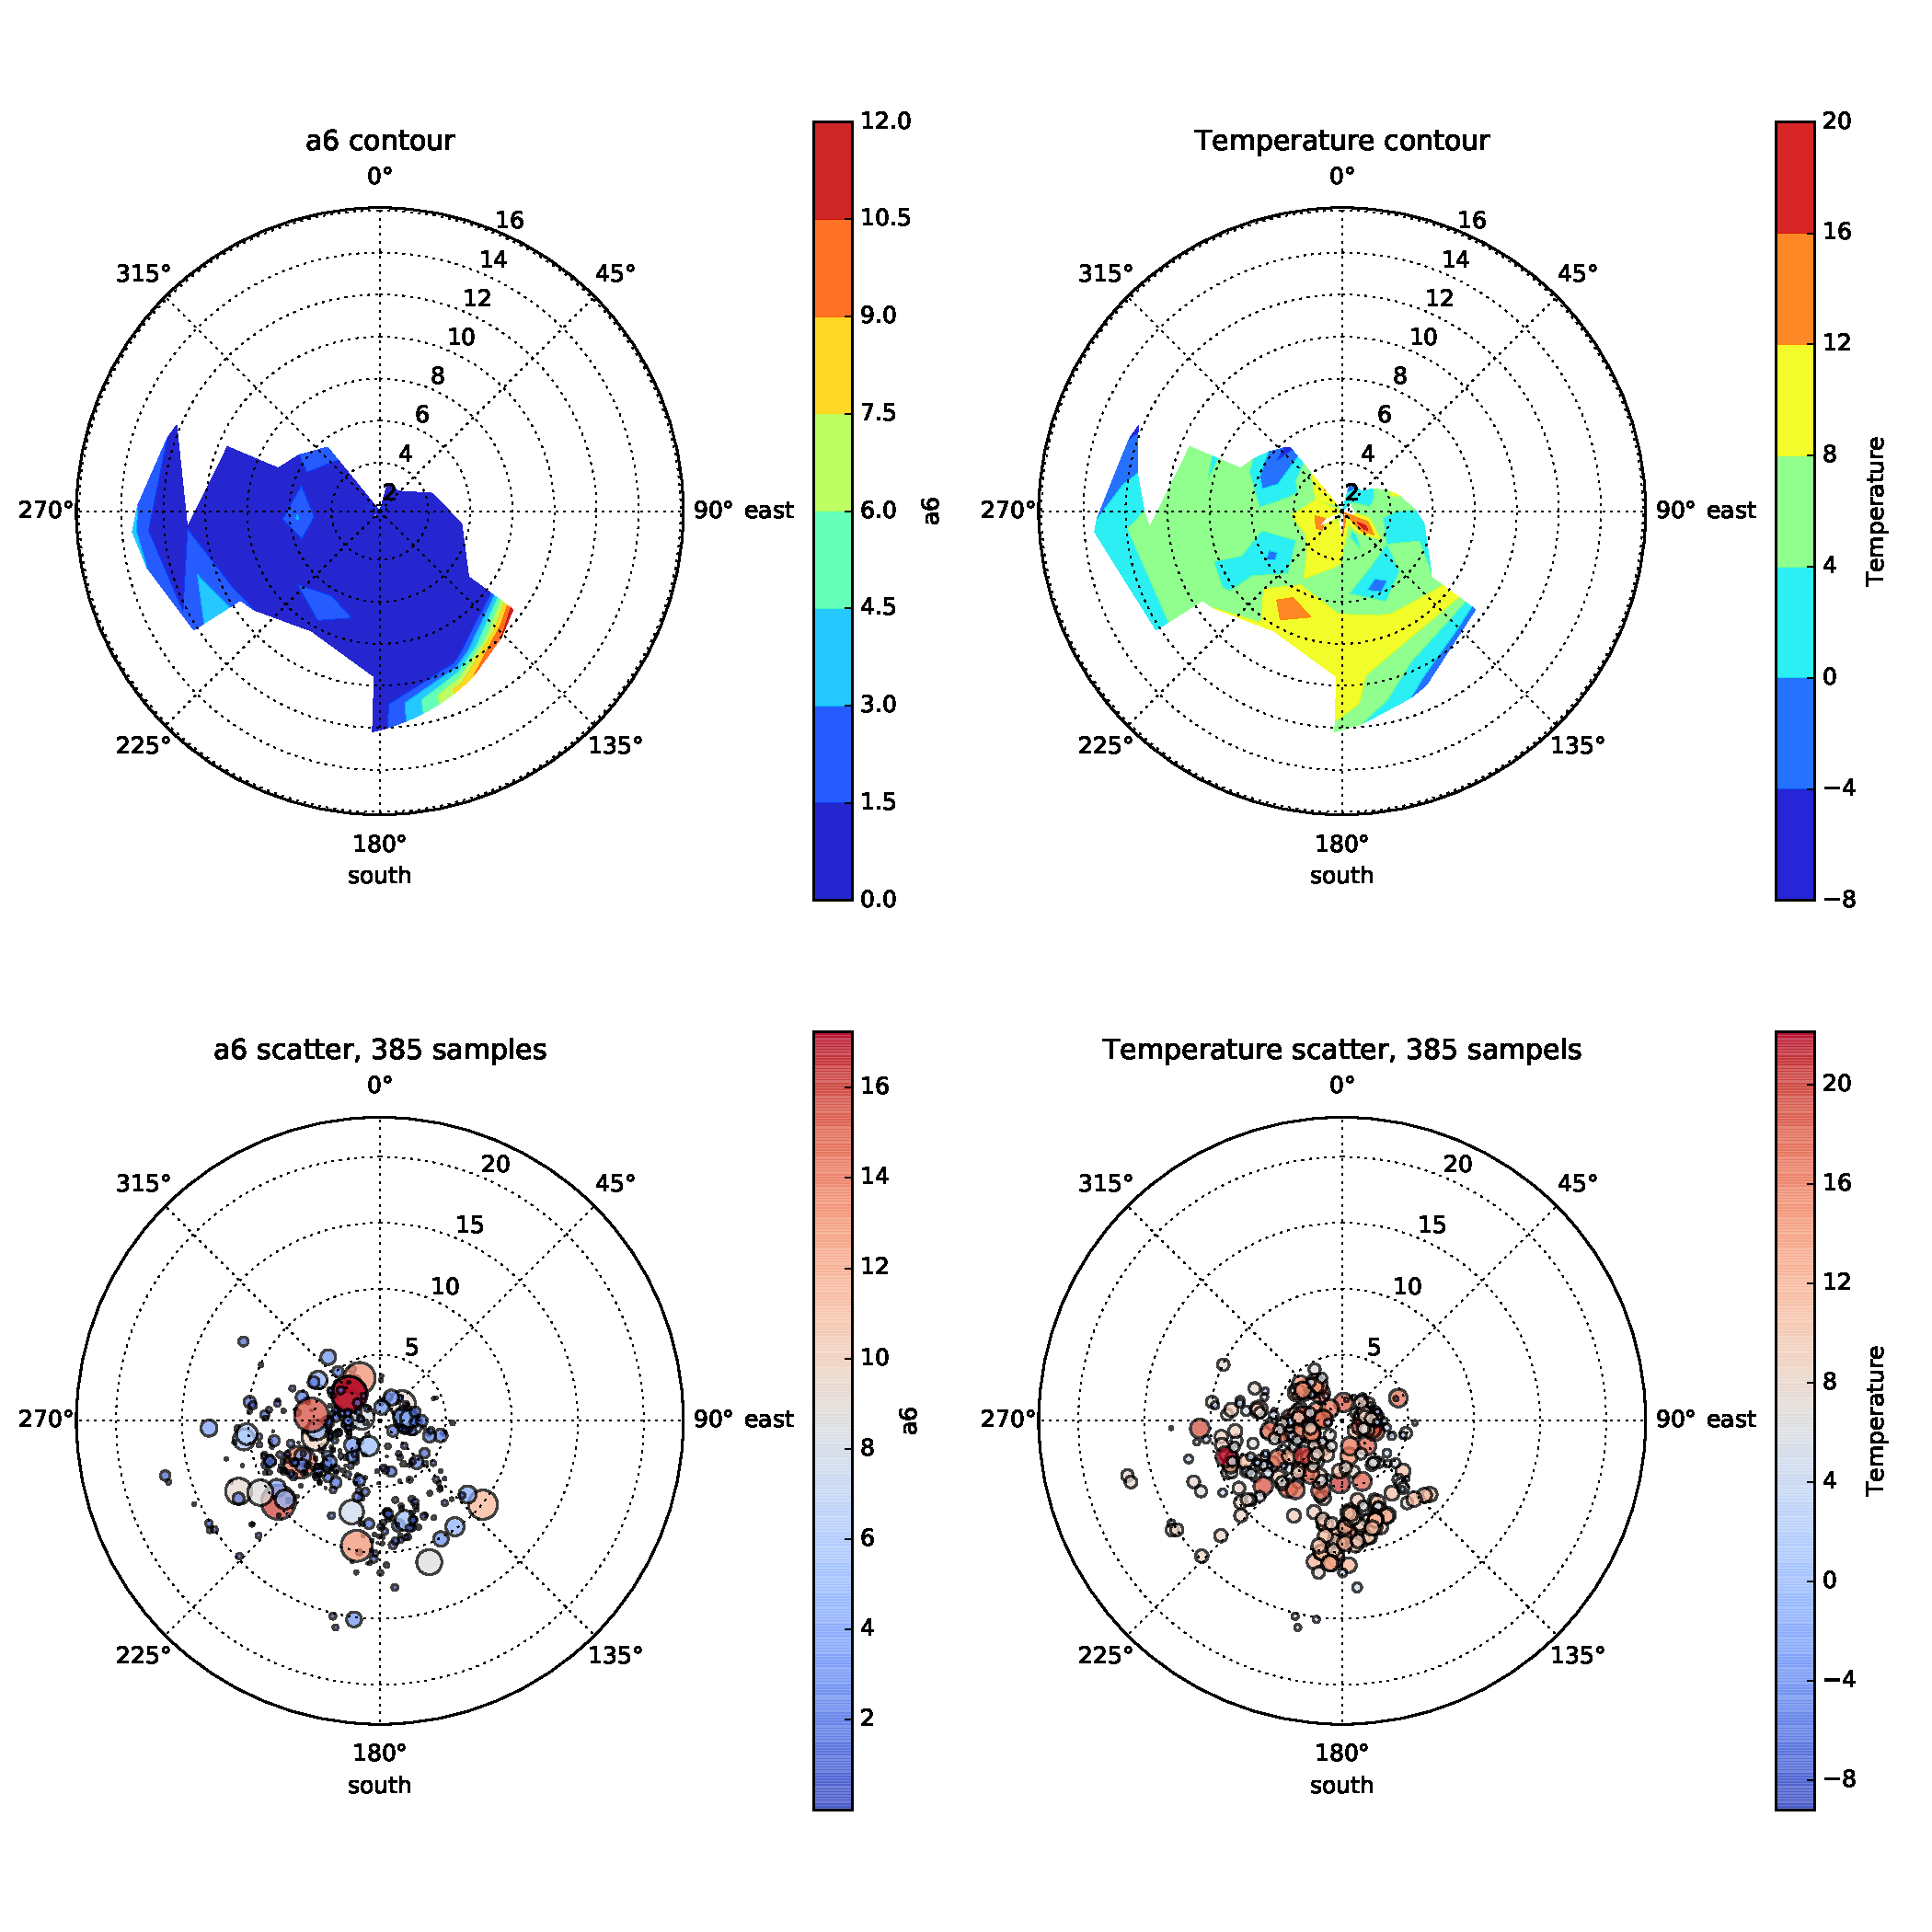
\includegraphics[scale=.46]{wind/wind_a6}
	\caption[Polarplot Windgeschwindigkeit, Windrichtung und $A_6$]{Polarplot Windgeschwindigkeit, Windrichtung und $A_6$}
    \label{wind_a6}
\end{figure}

\chapter{Quelltext}
Der komplette Quelltext ist im Softwarerepositorium zu finden.
\begin{mdframed}[style=emphasis]
	\centering
	\url{http://github.com/JeanElsner/focus-series}
\end{mdframed}
An dieser stelle soll nur Auszugsweise die Datei \emph{focus.py} aufgeführt werden, da sie das wesentliche Ergebnis dieser Arbeit darstellt. Die Datei implementiert den temperatur- und elevationsabhängigen Interpolanten der Fokusfunktion. Bildet also Temperatur und Elevation auf die Position des Sekundärspiegels entlang der optischen Achse ab.

\definecolor{mygreen}{rgb}{0,0.6,0}
\definecolor{mygray}{rgb}{0.5,0.5,0.5}
\definecolor{mymauve}{rgb}{0.58,0,0.82}

\lstset{ %
  backgroundcolor=\color{white},   % choose the background color; you must add \usepackage{color} or \usepackage{xcolor}
  basicstyle=\footnotesize,        % the size of the fonts that are used for the code
  breakatwhitespace=false,         % sets if automatic breaks should only happen at whitespace
  breaklines=true,                 % sets automatic line breaking
  captionpos=b,                    % sets the caption-position to bottom
  commentstyle=\color{mygreen},    % comment style
  deletekeywords={...},            % if you want to delete keywords from the given language
  escapeinside={\%*}{*)},          % if you want to add LaTeX within your code
  extendedchars=true,              % lets you use non-ASCII characters; for 8-bits encodings only, does not work with UTF-8
  frame=L,	                   % adds a frame around the code
  keepspaces=true,                 % keeps spaces in text, useful for keeping indentation of code (possibly needs columns=flexible)
  keywordstyle=\color{blue},       % keyword style
  language=Python,                 % the language of the code
  otherkeywords={*,...},           % if you want to add more keywords to the set
  numbers=left,                    % where to put the line-numbers; possible values are (none, left, right)
  numbersep=5pt,                   % how far the line-numbers are from the code
  numberstyle=\tiny\color{mygray}, % the style that is used for the line-numbers
  rulecolor=\color{black},         % if not set, the frame-color may be changed on line-breaks within not-black text (e.g. comments (green here))
  showspaces=false,                % show spaces everywhere adding particular underscores; it overrides 'showstringspaces'
  showstringspaces=false,          % underline spaces within strings only
  showtabs=false,                  % show tabs within strings adding particular underscores
  stepnumber=1,                    % the step between two line-numbers. If it's 1, each line will be numbered
  stringstyle=\color{mymauve},     % string literal style
  tabsize=2,	                   % sets default tabsize to 2 spaces
  title=\lstname                   % show the filename of files included with \lstinputlisting; also try caption instead of title
}

\section{focus.py}
\label{focus.py}

\lstinputlisting[language=Python]{focus.py}

\end{appendix}
